\documentclass{beamer}

\graphicspath{{scn-slides//}{figures//}}

\makeatletter
\def\input@path{{scn-slides}}
\makeatother

\usepackage{scn-slides}
\usepackage{comment}

\begin{document}

\title{Курс лекций по дисциплине\\ Математические основы интеллектуальных систем}   
\author[]{Шункевич Д.В.}
\institute[]{Белорусский государственный университет информатики и радиоэлектроники}

\begin{frame}
    \titlepage
\end{frame}

%Knowledge representation

\title{Лекция 1\\Основные положения семантической технологии проектирования интеллектуальных компьютерных систем нового поколения \vspace{-2em}} 
\author[]{Шункевич Д.В.}
\institute[]{Белорусский государственный университет информатики и радиоэлектроники}

\begin{frame}
	\titlepage
\end{frame}

\begin{frame}{\\Содержание лекции}
	\topline
	\justifying
	\begin{itemize}
		\item[--] Понятие интеллекта, интеллектуальной системы, комплексной задачи.
		\item[--] Основные положения семантической технологии проектирования интеллектуальных компьютерных систем нового поколения.
		\item[--] Основные компоненты указанной технологии.
		\item[--] Понятие информационной конструкции, формального языка, знака, синтаксиса, семантики.
		\item[--] Понятие семантической памяти.
	\end{itemize}
\end{frame}

\begin{frame}{\\Что такое "интеллект"?}
	\vspace{10mm}
	Интеллектуальная система (ИС) -- система, которая может легко научиться решать новые задачи. То есть основной признак интеллектуальности -- обучаемость.\\ \vspace{5mm}
	Важно отличать:
	\begin{itemize}
		\item[--] способность обучаться более качественному решению задач определенного ограниченного класса (как это делают классические нейросетевые модели) \\
		\item[--] способность относительно легко переходить от решения задач одного класса к решению задач другого класса (с ограничениями или без них).
	\end{itemize}
\end{frame}

\begin{frame}{\\Что такое комплексная задача?}
	Комплексная задача - задача, для решения которой необходимо использовать различные виды заний и различные модели решения задач. \\ \vspace{3mm}
	Более того, невозможно заранее сказать, какой набор моделей потребуется для решения конкретной задачи. \\
	\vspace{5mm}
	Примеры комплексных задач:
	\begin{itemize}
		\item[--] понимание естественных языков, изображений, речевых сообщений \\
		\item[--] планирование поведения интеллектуальных роботов.
	\end{itemize}
\end{frame}

\begin{frame}{\\Гибридная интеллектуальная система}
	Гибридная интеллектуальная система (ГИС) -- интеллектуальная система, интегрирующая различные виды знаний и различные модели решения задач.\\
	Именно ГИС способны решать комплексные задачи. Однако у современных ГИС существует ряд недостатков:
	\begin{itemize}
		\item[--] монолитность 
		\item[--] решение конкретной задачи, а не различных классов задач
		\item[--] разработка требует колоссальных ресурсов
		\item[--] практически невозможно повторно использовать какие-либо компоненты систем для решения других задач, необходимо все делать заново
	\end{itemize}
\end{frame}

\begin{frame}{\\Что такое OSTIS?}
	\vspace{5mm}
	OSTIS (Open Semantic Technology for Intelligent Systems) – \textit{открытая} комплексная технология проектирования \textit{совместимых} интеллектуальных систем.\\
	Основные положения:
		\begin{itemize}
		\item[--] база знаний (БЗ) OSTIS может описывать любой вид знаний
		\item[--] решатель задач OSTIS основан на многоагентном подходе и позволяет легко комбинировать любые модели решения задач
		\item[--] интерфейс ostis-системы представляет собой подсистему со своей БЗ и решателем задач (также может быть описан с помощью SC-кода)
		\item[--] использование универсального способа представления (кодирования) информации, получившего название SC-код 
	\end{itemize}
\end{frame}


\begin{frame}{\\Достоинства OSTIS}
	\begin{itemize}
		\item[--] универсальность и унифицированность (единообразие) представления (любая информация может быть представлена одним и тем же способом)
		\item[--] удобство машинной обработки и восприятия человеком
		
	\end{itemize}
\end{frame}


\begin{frame}{\\}
	
\end{frame}
\title{Лекция 2\\Базовый язык представления знаний}   
\author[]{Шункевич Д.В.}
\institute[]{Белорусский государственный университет информатики и радиоэлектроники}

\begin{frame}
	\titlepage
\end{frame}

\begin{frame}{\\Содержание лекции}
	\topline
	\justifying
	\begin{itemize}
	\item[--] Основные положения базового языка представления знаний в интеллектуальных системах – SC-кода. 
	\item[--] Алфавит, синтаксис, базовая денотационная семантика SC-кода. 
	\item[--] Синтаксическая и семантическая классификация sc-элементов.
	\end{itemize}
\end{frame}


\begin{frame}{\\Semantic Computer code = SC-code}
	SC-code основан на \textit{теории графов} (синтаксис) и \textit{теории множеств} (семантика), что позволяет единообразно представлять различные виды знаний, удобно их хранить и обрабатывать.
\end{frame}

\begin{frame}{\\Сравнение языков представления знаний и информации}
	\begin{columns}[T,onlytextwidth]
		\begin{column}{0.5\textwidth}
			\begin{itemize}
				\item Язык с алфавитом \{0, 1\}
				\begin{itemize}
					\item[--] не удобен для человека
					\item[--] удобен для обработки в компьютере
					\item[--] нельзя понять информацию без контекста
					\item[--] легко реализовать
				\end{itemize}
			\end{itemize}
		\end{column}
		\begin{column}{0.5\textwidth}
			\begin{itemize}
				\item SC-code
				\begin{itemize}
					\item[--] удобен для человека
					\item[--] удобен для обработки в компьютере
					\item[--] обладает «осмысленностью»
				\end{itemize}
			\end{itemize}
		\end{column}
	\end{columns}
	\vspace{5mm}
	Переход к "новому качеству" в области информационных технологий будет обусловлен переходом от обработки данных к обработке знаний.
	\\ From data science to knowledge science
\end{frame}

\begin{frame}{\\Формы внешнего представления SC-кода}
	\vspace{10mm}
	\begin{columns}[T,onlytextwidth]
		\begin{column}{0.5\textwidth}
			\begin{itemize}
				\item SCs -- Semantic Code string \\ (Язык линейного представления знаний) \vspace{10mm}
				\item SCn -- Semantic Code natural \\ (Язык структурированного представления знаний) \vspace{10mm}
				\item SCg -- Semantic Code graphic \\ (Язык графического представления знаний) 
			\end{itemize}
		\end{column}
		\begin{column}{0.56\textwidth}
			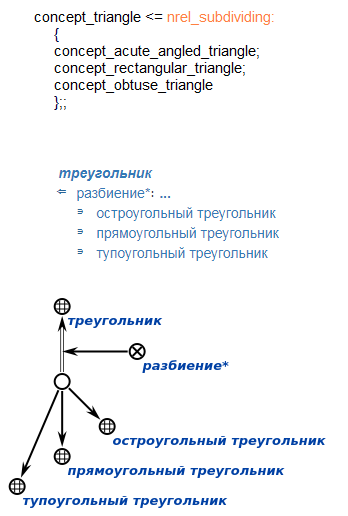
\includegraphics[width=50mm]{./part1/pictures/ostis-basics-1.png}
		\end{column}
	\end{columns}
\end{frame}

\begin{frame}{\\Информация VS знания}
	\vspace{10mm}
	Данные -- набор значений (фактов, цифр и т.д.)\\
	Пример: статистика кликов пользователя на элементы управления заданного сайта \\
	\vspace{5mm}
	Информация -- любые сведения об окружающем мире независимо от формы их представления \\
	Пример: голосовое сообщение \\
	Пример: номер телефона \\
	\vspace{5mm}
	Знания -- семантически и синтаксически целостная информация \\
	Пример: теорема Пифагора \\
	Пример: рецепт приготовления торта «Наполеон»
\end{frame}




\begin{frame}{\\Информация VS знания}
	\vspace{10mm}
	\begin{columns}[T,onlytextwidth]
		\begin{column}{0.5\textwidth}
			\vspace{20mm}
			Одна из ключевых отличительных особенностей знаний – интерпретируемость. \\
			(Дмитрий Александрович Поспелов)
		\end{column}
		\begin{column}{0.5\textwidth}
			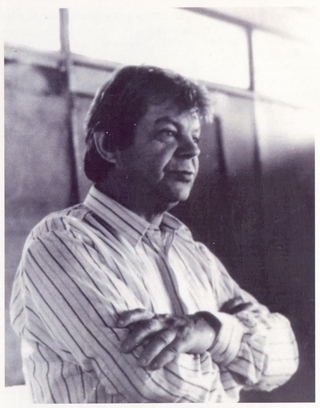
\includegraphics[width=50mm]{./part1/pictures/sc-code-pospelov.jpg}
		\end{column}
	\end{columns}
\end{frame}


\begin{frame}{\\Семантические сети}
	Семантическая сеть -- граф, вершины которого являются знаками некоторых сущностей, а дуги (ребра) – знаками связей между этими сущностями
	\\
	Семантика знака -- отношение между знаком и сущностью (значением знака, денотатом), которую он обозначает.
	\\
	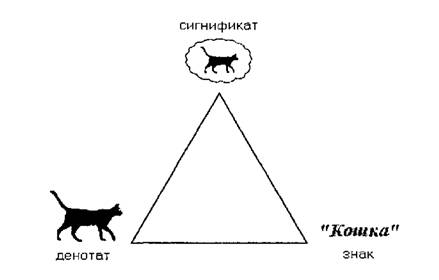
\includegraphics[width=50mm]{./part1/pictures/sc-code-cat.jpg}
\end{frame}

\title{Лекция 3\\Внешние информационные конструкции}   
\author[]{Шункевич Д.В.}
\institute[]{Белорусский государственный университет информатики и радиоэлектроники}

\begin{frame}
	\titlepage
\end{frame}

\begin{frame}{\\Содержание лекции}
	\topline
	\justifying
	Понятие внешней информационной конструкции, классификация. Понятие внутреннего файла базы знаний, классификация. Понятие идентификатора, типология идентификаторов. Примеры формализации идентификаторов.
\end{frame}

\begin{frame}{\\Информационная конструкция}
	\topline
	\justifying
	\begin{SCn}
		\scnheader{информационная конструкция}
		\scnidtf{конструкция (структура), содержащая некоторые сведения о некоторых сущностях}
		\scnidtf{информационная модель, состоящая из некоторого множества различных \textit{знаков}, обозначающих моделируемые (описываемые) \textit{сущности} любого вида и, в частности, \textit{знаков}, обозначающих различного вида связи между знаками описываемых \textit{сущностей} (такие связи чаще всего являются отражениями (моделями) связей между \textit{сущностями}, которые обозначаются связываемыми \textit{знаками})}
		\scntext{примечание}{Форма представления ("изображения"{}, "материализации"{}), форма структуризации (синтаксическая структура), а также \textit{смысл*} (денотационная семантика) \textit{информационных конструкций} могут быть самыми различными.}
	\end{SCn}
	
\end{frame}

\begin{frame}{\\Дискретная информационная конструкция}
	\topline
	\justifying
	\begin{SCn}
		\footnotesize
		\scnheader{дискретная информационная конструкция}
		\scnsubset{информационная конструкция}
		\scntext{\textit{пояснение}}{Каждая дискретная информационная конструкция -- это информационная конструкция, смысл которой задается
		\begin{textitemize}
			 \item множеством элементов (синтаксически атомарных фрагментов) этой информационной конструкции
			 \item алфавитом этих элементов -- семейством классов синтаксически эквивалентных элементов информационной конструкции
			 \item принадлежностью каждого элемента информационной конструкции соответствующему классу синтаксически эквивалентных элементов информационной конструкции
			 \item конфигурацией связей инцидентности между элементами информационной конструкции
		 \end{textitemize}}
	\end{SCn}
	
\end{frame}

\begin{frame}{\\Информационные конструкции}
	\topline
	\justifying
	\begin{SCn}
		\scnheader{информационная конструкция}
		\begin{scnrelfromset}{\textit{разбиение}}
			\scnitem{внутренняя информационная конструкция}
			\begin{scnindent}
			\scnidtf{информационная конструкция, хранимая в памяти некоторой кибернетической системы, и непосредственно интерпретируемая (понимаемая) решателем задач этой системы}
			\end{scnindent}
			\scnitem{внешняя информационная конструкция}
			\begin{scnindent}
			\scnidtf{информационная конструкция, представленная на каком-либо внешнем носителе или в памяти другой кибернетической системы}
			\end{scnindent}
			\scnitem{файл}
			\begin{scnindent}
			\scnidtf{первичный электронный образ некоторой внешней информационной конструкции}
			\end{scnindent}
		\end{scnrelfromset}
	\end{SCn}
	
\end{frame}

\begin{frame}{\\Файл}
	\topline
	\justifying
	\begin{SCn}
		\scnheader{файл}
		\scnidtf{информационная конструкция, которая не является sc-конструкцией и которая может храниться в файловой памяти ostis-системы}
		\scntext{\textit{примечание}}{файловая память \textit{ostis-системы}, хранящая различного рода \textit{информационные конструкции} (образы, модели), не являющиеся \textit{sc-конструкциями}, должна быть тесно связана с \textit{sc-памятью} этой же \textit{ostis-системы}. Как минимум, каждый файл \textit{ostis-системы} должен быть связан с тем \textit{sc-элементом}, которых является знаком этого файла (точнее, знаком синглетона, элементом которого является указанный файл)}
		
	\end{SCn}
	
\end{frame}

\begin{frame}{\\Файл}
	\topline
	\justifying
	\vspace*{\fill}\\
	\small{
		\begin{SCn}
		\scnheader{файл}
		\scnidtf{sc-узел, обозначающий файл}
		\scnidtf{знак файла}
		\begin{scnrelfromset}{\textit{разбиение}}
			\scnitem{ея-файл}
			\begin{scnindent}
				\scnidtf{естественно-языковой файл}
			\end{scnindent}
			\scnitem{файл, являющийся текстом формального языка}
			\begin{scnindent}
				\scnsuperset{sc.g-файл}
				\scnsuperset{sc.n-файл}
				\scnsuperset{sc.s-файл}
			\end{scnindent}
			\scnitem{файл, отражающий процесс изменения sc.g-текста}
			\scnitem{графический файл}
			\scnitem{файл-изображение}
			\scnitem{видео-файл}
			\scnitem{аудио-файл}
		\end{scnrelfromset}
		
	\end{SCn}
}
	
\end{frame}

\begin{frame}{\\Файл}
	\topline
	\justifying
	\vspace*{\fill}\\
	\small{
	\begin{SCn}
		\scnheader{файл}
		\begin{scnrelfromset}{\textit{разбиение}}
			\scnitem{файл-экземпляр}
			\begin{scnindent}
				\scnidtf{файл, являющийся конкретным электронным документом или электронным образом конкретной внешней информационной конструкции}
			\end{scnindent}
			\scnitem{файл-образец}
			\begin{scnindent}
				\scnidtf{файл-класс \textit{ostis-системы}}
				\scnidtf{файл, являющийся одновременно также и знаком множества всевозможных экземпляров (копий) этого файла}
			\end{scnindent}
		\end{scnrelfromset}
		\begin{scnrelfromset}{\textit{разбиение}}
			\scnitem{внешний файл ostis-системы}
			\scnitem{\textbf{внутренний файл ostis-системы}}
		\end{scnrelfromset}
		
	\end{SCn}
}
\end{frame}

\begin{frame}{\\Файл}
	\topline
	\justifying
	\begin{SCn}
		\scnheader{файл}
		\scntext{\textit{примечание}}{Представление \textit{информационных конструкций} в виде файлов ориентировано на представление \textit{дискретных (!) информационных конструкций}. Поэтому "файловое" представление \textit{недискретных информационных конструкций} (например, различного рода сигналов) предполагает "дискретизацию" таких конструкций, т.е. преобразование их в \textit{дискретные}. Так преобразуются аудио-сигналы (в частности, речевые сообщения), изображения, видео-сигналы и др.}
		
	\end{SCn}
	
\end{frame}

%Addition
\iffalse
\begin{frame}{\\Внутренний файл}
	\topline
	\justifying
	\begin{SCn}
		\footnotesize
		\scnheader{внутренний файл ostis-системы}
		\scniselement{синтаксически выделяемый класс sc-элементов в рамках SC-кода}
		\scniselement{семантически выделяемый класс sc-элементов в рамках SC-кода}
		\scntext{\textit{примечание}}{Данный класс sc-элементов, являющихся знаками файлов, хранимых в памяти \textit{ostis-систем}, в отличие от других синтаксически выделяемых классов \textit{sc-элементов}, представляет собой одновременно синтаксически и семантически выделяемый класс \textit{sc-элементов}. Это обусловлено тем, что 
		\begin{textitemize}
			\item каждый экземпляр данного класса \textit{sc-элементов} является знаком конкретного файла, хранимого в памяти \textit{ostis-системы}
			\item каждый файл, хранимый в памяти \textit{ostis-системы}, может и должен быть обозначен только таким \textit{sc-элементом}, который является экземпляром рассматриваемого класса \textit{sc-элементов}.
		\end{textitemize}}
	\end{SCn}
\end{frame}
\fi

\begin{frame}{\\Внутренний файл}
	\topline
	\justifying
	\begin{SCn}
		\scnheader{внутренний файл ostis-системы}
		\scntext{\textit{примечание}}{sc-узел может быть знаком файла, находящегося в памяти другой ostis-системы (не в той, в которой хранится этот sc-узел). Но в этом случае указанный sc-узел не будет принадлежать рассматриваемому
		классу sc-узлов.}
		\scntext{\textit{примечание}}{Следует отличать синтаксическую эквивалентность файлов, семантическую эквивалентность файлов и совпадение файлов (когда речь идет об одном и том же файле). Т.е. копия файла и один и тот же файл – это разные вещи}
	\end{SCn}
	
\end{frame}

\begin{frame}{\\Идентификатор}
	\topline
	\justifying
	\begin{SCn}
		\scnheader{sc-идентификатор}
		\scnidtf{строка символов или пиктограмма, взаимно однозначно представляющая соответствующий \textit{sc-элемент}, хранимый в \textit{sc-памяти}}
		\scnidtf{внешний идентификатор \textit{sc-элемента}}
		\begin{scnrelfromset}{\textit{разбиение}}
			\scnitem{простой sc-идентификатор}
			\begin{scnindent}
				\scnidtf{простой внешний идентификатор \textit{sc-элемента}}
			\end{scnindent}
			\scnitem{sc-выражение}
			\begin{scnindent}
				\scnidtf{сложный внешний идентификатор \textit{sc-элемента}, в состав которого входит один или несколько идентификаторов других \textit{sc-элементов}}
			\end{scnindent}
		\end{scnrelfromset}
	\end{SCn}
	
\end{frame}

\begin{frame}{\\Идентификатор}
	\topline
	\justifying
	\vspace*{\fill}\\
	\scriptsize{
	\begin{SCn}
		\scnheader{sc-идентификатор}
		\begin{scnrelfromset}{\textit{разбиение}}
			\scnitem{основной sc-идентификатор}
			\begin{scnindent}
				\scnidtf{основной \textit{sc-идентификатор} для носителей дополнительно указываемого языка общения (например, соответствующего естественного языка)}
				\scntext{\textit{примечание}}{основной \textit{sc-идентификатор} является уникальным (не имеет синонимов и омонимов) в рамках соответствующего естественного языка}
				\scnsuperset{основной международный \textit{sc-идентификатор}}
			\end{scnindent}
			\scnitem{неосновной sc-идентификатор}
			\begin{scnindent}
				\scnsuperset{(неосновной \textit{sc-идентификатор} $\cap$ пояснение)}
				\begin{scnindent}
					\scnidtf{неосновной \textit{sc-идентификатор}, являющийся одновременно и пояснением обозначаемой сущности}
					\scnsuperset{(неосновной \textit{sc-идентификатор} $\cap$ определение)}
					\begin{scnindent}
						\scnidtf{неосновной \textit{sc-идентификатор}, являющийся одновременно и определением обозначаемого понятия}
					\end{scnindent}
				\end{scnindent}
				\scnsuperset{неосновной часто используемый sc-идентификатор}
			\end{scnindent}
		\end{scnrelfromset}
	\end{SCn}
}
	
\end{frame}

\begin{frame}{\\Неосновной sc-идентификатор}
	\topline
	\justifying
	С помощью неосновных sc-идентификаторов указываются возможные \textit{синонимы*} соответствующего \textit{основного sc-идентификатора}, которые в частности, могут пояснять или даже определять обозначаемую сущность, указывает на важные свойства этой сущности.

	\bigskip
	Для некоторых sc-элементов могут часто использоваться не только основные, но и неосновные sc-идентификаторы (особенно в неформальных текстах -- в пояснениях, примечаниях и т.п.). Явное выделение такого класса sc-идентификаторов позволяет упростить семантический анализ исходных текстов баз знаний.
\end{frame}

\begin{frame}{\\Основной sc-идентификатор}
	\topline
	\justifying
	\begin{SCn}
		\scnheader{основной sc-идентификатор}
		\scnsubset{файл-образец ostis-системы}
		\scnrelboth{\textit{семантическая эквивалентность}}{\scnfilelong{Все основные идентификаторы \textit{sc-элементов} в памяти \textit{ostis-системы} оформляются в виде копируемых фалов-образцов \textit{ostis-системы}.}}
		\begin{scnindent}
			\scntext{пояснение}{Копии основных \textit{sc-идентификаторов} входят в состав внешних текстов различных языков (\mbox{SCg-кода}, SCs-кода, SCn-кода), а также в различных падежах, склонения, спряжениях в состав файлов \textit{ostis-систем}.}
		\end{scnindent}
	\end{SCn}
	
\end{frame}

\begin{frame}{\\Построение основных sc-идентификатор}
	\topline
	\justifying
	В качестве \textit{основных sc-идентификаторов} могут использоваться также общепринятые международные условные обозначения некоторых сущностей, например, обозначения часто используемых функций (sin, cos, tg, log, и т.д.), единиц измерения, денежных единиц и многое другое. Формально каждый основной международный sc-идентификатор считается основным sc-идентификатором также и для каждого естественного языка, несмотря на то, что символы, используемые в основных международных sc-идентификаторах, могут не соответствовать алфавиту некоторых или даже всех естественных языков.
\end{frame}

\begin{frame}{\\Идентификатор}
	\topline
	\justifying
	\vspace*{\fill}\\
	\footnotesize{
	\begin{SCn}
		\scnheader{sc-идентификатор}
		\begin{scnrelfromset}{разбиение}
			\scnitem{строковый sc-идентификатор}
			\begin{scnindent}
				\scnidtf{\textit{sc-идентификатор}, представленный строкой символов, которая является именем обозначаемой сущности}
				\scnidtf{имя сущности, обозначаемой идентифицируемым \textit{sc-элементом}}
				\scnidtf{имя (термин, словосочетание), синонимичное соответствующему (идентифицируемому) \mbox{sc-элементу} и представленное в соответствующем алфавите символов}
			\end{scnindent}
			\scnitem{нестроковый sc-идентификатор}	
			\begin{scnindent}
				\scntext{пояснение}{В общем случае в качестве \textit{sc-идентификатора} некоторого \textit{sc-элемента} может выступать произвольный \textit{внутренний файл ostis-системы}, например, пиктограмма, условное обозначение или даже аудиофрагмент.}	
			\end{scnindent}
		\end{scnrelfromset}
		\scntext{примечание}{Введенные нами \textit{sc-идентификаторы} используются во всех внешних языках, близких SC-коду -- в SCg-коде, в SCs-коде и в SCn-коде.}
	\end{SCn}
}
	
\end{frame}


\begin{frame}{\\Строковый sc-идентификатор}
	\topline
	\justifying
	\small{
	\begin{SCn}
		\scnheader{строковый sc-идентификатор}
		\scnidtf{имя, приписываемое идентифицируемому \textit{sc-элементу}}
		\scnidtf{имя сущности, обозначаемой идентифицируемым \textit{sc-элементом}}
		\scnidtf{строка символов, синонимичная соответствующему идентифицируемому \textit{sc-элементу}}
		\scnsuperset{основной строковый sc-идентификатор}
		\begin{scnindent}
			\scnidtf{уникальное для каждого естественного языка внешнее имя, приписываемое идентифицируемому \textit{sc-элементу}}
			\scnsuperset{основной русскоязычный sc-идентификатор}
			\scnsuperset{системный sc-идентификатор}
			\scnsuperset{основной англоязычный sc-идентификатор}
			\scnsuperset{основной германоязычный sc-идентификатор}
			\scnsuperset{основной франкоязычный sc-идентификатор}
			\scnsuperset{основной италоязычный sc-идентификатор}
			\scnsuperset{основной китайскоязычный sc-идентификатор}
		\end{scnindent}
		\scnsuperset{системный sc-идентификатор}
	\end{SCn}
}
	
\end{frame}

\begin{frame}{\\Системный sc-идентификатор}
	\topline
	\justifying
	\begin{SCn}
		\scnheader{системный sc-идентификатор}
		\scnidtf{\textit{sc-идентификатор}, являющийся уникальным в рамках всей базы знаний \textit{Экосистемы OSTIS} (Глобальной базы знаний).}
		\scntext{пояснение}{Данный \textit{sc-идентификатор}, как правило, используется в исходных текстах базы знаний, при обмене сообщениями между \textit{ostis-системами}, а также для взаимодействия \textit{ostis-системы} с компонентами, реализованными с использованием средств, внешних с точки зрения \textit{Технологии OSTIS}, например, программ, написанных на традиционных языках программирования. Алфавит системных \textit{sc-идентификаторов} максимально упрощен для того, чтобы обеспечить удобство автоматической обработки таких \textit{sc-идентификаторов} с использованием современных технических средств, в частности, запрещены пробелы и различные специальные символы.}
	\end{SCn}
	
\end{frame}

\begin{frame}{\\Построение системных sc-идентификаторов}
	\topline
	\justifying
	\vspace*{\fill}\\
	\footnotesize
	Символами, использующимися в \textit{системном sc-идентификаторе}, могут быть буквы латинского алфавита, цифры, знак нижнего подчеркивания и знак тире. Для обеспечения интернационализации рекомендуется формировать \textit{системные sc-идентификаторы} на основании основных англоязычных \textit{sc-идентификаторов}.
	
	\bigskip
	Таким образом, наиболее целесообразно формировать \textit{системный sc-идентификатор} \textit{sc-элемента} из основного англоязычного путем замены всех символов, не входящих в описанный выше алфавит на символ нижнее подчеркивание (``\_''). Кроме того, заглавные буквы чаще всего заменяются на соответствующие строчные.

	\bigskip	
	Для именования sc-элементов, являющихся знаками \textit{ролевых отношений}, вместо знака ``\scnrolesign'' в \textit{системном sc-идентификаторе} используется приставка ``rrel'' и далее после нижнего подчеркивания записывается имя \textit{ролевого отношения}.
	
\end{frame}

\begin{frame}{\\Построение системных sc-идентификаторов}
	\topline
	\justifying
	\vspace*{\fill}\\
	 Для именования sc-элементов, являющихся знаками \textit{неролевых отношений}, вместо знака ``*'' в \textit{системном sc-идентификаторе} используется приставка ``nrel'' и далее после нижнего подчеркивания записывается имя \textit{неролевого отношения}.\\

	\bigskip	
	Для именования sc-элементов, являющихся знаками классов \textit{понятий}~~в~~\textit{системном sc-идентификаторе} используется приставка ``concept'' и далее после нижнего подчеркивания записывается имя \textit{класса}.\\

	\bigskip
	Для именования sc-элементов, являющихся знаками \textit{структур}~~в~~\textit{системном sc-идентификаторе} используется приставка ``struct'' и далее после нижнего подчеркивания записывается имя \textit{структуры}.
\end{frame}

\begin{frame}{\\Нетранслируемый sc-идентификатор}
	\topline
	\justifying
\begin{SCn}
	\scnheader{нетранслируемый sc-идентификатор}
	\scnsubset{системный sc-идентификатор}
	\scnidtf{\textit{sc-идентификатор}, не представляемый в базе знаний \textit{ostis-системы}}
	\scnidtf{\textit{sc-идентификатор}, существующий только вне базы знаний \textit{ostis-системы}}	
\end{SCn}
	
\end{frame}

\begin{frame}{\\Нетранслируемый sc-идентификатор}
	\topline
	\justifying
	\vspace*{\fill}\\
	\footnotesize
	Нетранслируемые sc-идентификаторы используются только в рамках исходных текстов \textit{баз знаний} (в том числе, \textit{sc.s-текстов}) и при обмене сообщениями между \textit{ostis-системами} в тех случаях, когда необходимо в нескольких фрагментах исходного текста \textit{базы знаний} или передаваемого сообщения использовать имя одного и того же \textit{sc-элемента}, но при этом указанный \textit{sc-элемент} не имеет \textit{системного sc-идентификатора} и вводить его нецелесообразно.

	\bigskip
	Использование \textit{нетранслируемых sc-идентификаторов} позволяет повысить читабельность и структурированность исходных текстов \textit{баз знаний}, а также позволяет обратиться к одному и тому же неименуемому (в рамках базы знаний) \textit{sc-элементу} в разных файлах исходных текстов \textit{баз знаний} или в разных сообщениях, передаваемых между \textit{ostis-системами}. В качестве таких \textit{sc-элементов} часто выступают знаки \textit{структур} и \textit{связок}.

	\bigskip
	Таким образом, \textit{нетранслируемые sc-идентификаторы} существуют только вне \textit{базы знаний ostis-системы} и при формировании базы знаний из исходных текстов или при погружении в базу знаний полученного сообщения соответствующий им \textit{внутренний файл ostis-системы} не создается.
\end{frame}

\begin{frame}{\\Отличия идентификаторов}
	\topline
	\justifying
	\vspace*{\fill}\\
	\small
	Системные идентификаторы отличаются от основных, во-первых, требованием к уникальности в рамках всей базы знаний \textit{Экосистемы OSTIS} (а, значит, независимостью от внешнего языка), а во-вторых, более простым алфавитом, удобным для автоматической обработки.
	
	\bigskip
	\textit{Системные sc-идентификаторы} и \textit{нетранслируемые sc-идентификаторы} выполняют схожие функции, связанные с именованием \textit{sc-элементов} на уровне исходных текстов \textit{баз знаний} или передаваемых между \textit{ostis-системами} сообщений.

	\bigskip		
	Каждый \textit{системный sc-идентификатор} представляется в базе знаний в виде \textit{внутреннего файла ostis-системы} и связан с соответствующим \textit{sc-элементом} парой отношения \textit{системный \mbox{sc-идентификатор*}}. \textit{Нетранслируемые\\ sc-идентификаторы} не представляются в рамках \textit{базы знаний}, не имеют соответствующих \textit{внутренних файлов ostis-системы} и на уровне \textit{базы знаний} никак не связаны с идентифицируемыми ими \textit{sc-элементами}.
\end{frame}

\begin{frame}{\\Простой sc-идентификатор}
	\topline
	\justifying
	\vspace*{\fill}\\
	Простой sc-идентификатор -- идентификатор sc-элемента, в состав которого идентификаторы других sc-элементов не входят и который не содержит \textit{транслируемую в SC-код} информацию об обозначаемой им сущности. 
	
	\bigskip
	Простой строковый sc-идентификатор -- простой sc-идентификатор, представляющий собой строку (цепочку) символов, которая является именем (названием) той же сущности, что и идентифицируемый sc-элемент. Простые строковые sc-идентификаторы являются наиболее распространенным видом идентификаторов, приписываемых sc-элементам.
\end{frame}


\begin{frame}{\\Простой sc-идентификатор}
	\topline
	\justifying
	\vspace*{\fill}\\
	\small{
	\begin{SCn}
	\scnheader{простой строковый sc-идентификатор}
	\scnsuperset{системный sc-идентификатор}
	\scnsuperset{простой строковый идентификатор sc-переменной}
	\begin{scnindent}
		\scnhaselementrole{пример}{\scnfilelong{\_var1}}
	\end{scnindent}
	\scnsuperset{простой строковый sc-идентификатор неролевого отношения}
	\begin{scnindent}
		\scnidtf{простой строковый идентификатор sc-узла, являющегося знаком неролевого отношения}
		\scnhaselementrole{пример}{\scnfilelong{включение множеств*}}
	\end{scnindent}
	\scnsuperset{простой строковый sc-идентификатор ролевого отношения}
	\begin{scnindent}
		\scnidtf{простой строковый идентификатор sc-узла, являющегося знаком ролевого отношения}
		\scnhaselementrole{пример}{\scnfilelong{слагаемое\scnrolesign}}
	\end{scnindent}
\end{SCn}
}
\end{frame}


\begin{frame}{\\Простой sc-идентификатор}
	\topline
	\justifying
	\vspace*{\fill}\\
	\scriptsize{
	\begin{SCn}
	\scnsuperset{простой строковый sc-идентификатор класса классов}
	\begin{scnindent}
		\scnidtf{простой строковый идентификатор sc-узла, являющегося знаком класса классов}
		\scnhaselementrole{пример}{\scnfilelong{длина\scnsupergroupsign}}
	\end{scnindent}
	\scnsuperset{sc-идентификатор внешнего файла ostis-системы}
	\begin{scnindent}
		\scnidtf{URL-идентификатор}
		\scnhaselementrole{пример}{\scnfilelong{"file:///home/user/image1.png"{}}}
		\begin{scnindent}
			\scntext{примечание}{Данный sc-идентификатор описывает абсолютный путь к файлу под названием "image1.png"{}}
		\end{scnindent}	
		\scnhaselementrole{пример}{\scnfilelong{"file://image1.png"{}}}
		\begin{scnindent}
			\scntext{примечание}{Данный sc-идентификатор описывает относительный путь к файлу под названием "image1.png"{}}
		\end{scnindent}	
		
		\scnhaselementrole{пример}{\scnfilelong{"https://conf.ostis.net/content/image1.png"{}}}
		\begin{scnindent}
			\scntext{примечание}{Данный sc-идентификатор описывает путь к файлу под названием "image1.png"{}, расположенному на удаленном сервере.}
		\end{scnindent}	
	\end{scnindent}
	\end{SCn}
}
\end{frame}


\begin{frame}{\\Простой sc-идентификатор}
	\topline
	\justifying
	\vspace*{\fill}\\
	\small{
		\textit{sc-идентификаторы} внешних файлов ostis-систем предназначены для описания местоположения внешних файлов ostis-систем и представляют собой строку символов, которая строится в соответствии со стандартом URL, а затем берется в двойные кавычки. Кавычки нужны для однозначности определения того, где начинается и заканчивается данный sc-идентификатор, поскольку в общем случае в URL разрешены пробелы. Целесообразность этого обусловлена тем, что sc-идентификаторы данного типа часто используются в файлах исходных текстов баз знаний ostis-систем.
		
		\bigskip
		\textit{sc-идентификаторы} внешних файлов ostis-систем с точки зрения Технологии OSTIS являются простыми строковыми sc-идентификаторами, хотя и могут содержать специальные символы, например "\%"{} или "/"{}. Это связано с тем, что указанные идентификаторы не несут в себе семантически значимой информации о свойствах самого sc-элемента, обозначаемого таким sc-идентификатором, а только информацию о его расположении в текущем состоянии внешнего мира ostis-системы.
	}
\end{frame}

\begin{frame}{\\Простой sc-идентификатор}
	\topline
	\justifying
	\vspace*{\fill}\\
	\textbf{Правила построения простых строковых sc-идентификаторов} включают в себя:
		\begin{textitemize}
			\item Алфавит символов, используемых в простых строковых\\ sc-идентификаторах;
			\item Префиксы и суффиксы, используемые в простых строковых\\ sc-идентификаторах;
			\item Разделители и ограничители, используемые в простых строковых sc-идентификаторах;
			\item Правила построения \textit{имен собственных} и \textit{имен нарицательных}, являющихся простыми строковыми sc-идентификаторами;
			\item Правила построения простых строковых sc-идентификаторов, определяемые различными классами идентифицируемых sc-элементов.
		\end{textitemize}
\end{frame}

\begin{frame}{\\Сложный sc-идентификатор}
	\topline
	\justifying
	\vspace*{\fill}\\
	
	\textbf{\textit{sc-выражение}} -- идентификатор, который не только обозначает соответствующую сущность, но также содержит информацию, представляющую собой по возможности однозначную спецификацию указанной сущности.
	
	Однозначную спецификацию сущности, которая является понятием, называют \underline{определением} этого понятия
\end{frame}

\begin{frame}{\\Сложный sc-идентификатор}
	\topline
	\justifying
	\vspace*{\fill}\\
	\scriptsize{
		\begin{SCn}
			\scnheader{sc-выражение}
			\scnidtf{имя соответствующей {\normalfont(}именуемой{\normalfont)} сущности построенное по принципу "та {\normalfont(}тот{\normalfont)}, которая {\normalfont(}который{\normalfont)} указываемым образом связана с другими указываемыми сущностями"{}}
			\scnidtf{выражение, идентифицирующее sc-элемент}
			\scnidtf{идентификатор sc-элемента, в состав которого входят другие идентификаторы и денотационная семантика которого точно определяется конкретным набором правил построения таких сложных (комплексных) идентификаторов, состоящих из определенным образом связанных между собой других идентификаторов}
			\scnidtf{сложный идентификатор, состоящий из других идентификаторов}
			\scnidtf{идентификатор, который представляет собой конструкцию, состоящую из нескольких других идентификаторов, а также из некоторых разделителей и ограничителей, и денотационная семантика которого \underline{однозначно} задается конфигурацией указанной конструкции}
			\scnidtf{сложный sc-идентификатор}
			\scnidtf{сложный (составной) внешний идентификатор sc-элемента}
			\scnidtf{выражение, идентифицирующее sc-элемент}
			\scnidtf{sc-идентификатор, в состав которого входит один или несколько простых sc-идентификаторов}
		\end{SCn}
	}
\end{frame}

\begin{frame}{\\Сложный sc-идентификатор}
	\topline
	\justifying
	\vspace*{\fill}\\
	\scriptsize
		\textbf{\textit{sc-выражение}} разбивается на:
		\begin{textitemize}
			\item \textit{sc-выражение неориентированного множества} -- sc-выражение, ограниченное фигурными скобками
			\item \textit{sc-выражение структуры} -- sc-выражение, обозначающее структуру, представленную на любом известном и легко определяемом языке (Русском, Английском, SCg-коде, SCs-коде, SCn-коде)
			
			\textit{sc-выражение структуры} обозначает структуру, содержащую sc-текст, семантически эквивалентный тому тексту (на некотором известном языке), который заключен в фигурные скобки. Чаще всего такой текст записывается на формальном языке, например, SCs-коде, и может быть автоматически однозначно интерпретирован. Возможна ситуация, когда указанный текст записан на менее неформальном языке, например, Русском, но в этом случае его автоматическая интерпретация значительно усложняется и в общем случае не всегда однозначна.
			
			В текущей реализации средств разработки исходных текстов баз знаний в соответствии с более старой версией правил простроения sc-выражений вместо фигурных скобок \textit{sc-выражение структуры} ограничивается квадратными скобками со звездочками ("[*"{} и "*]"{}).
		
			\item \textit{sc-выражение ориентированного множества} -- sc-выражение кортежа, ограничиваемое угловыми скобками и обозначающее упорядоченное (ориентированное) множество sc-элементов, порядок которых задаётся последовательностью перечисляемых их sc-идентификаторов.	
		\end{textitemize}	
\end{frame}

\begin{frame}{\\Сложный sc-идентификатор}
	\topline
	\justifying
	\vspace*{\fill}\\
	\scriptsize
		\begin{textitemize}
			\item \textit{sc-выражение внутреннего файла ostis-системы} -- sc-выражение, обозначающее \textit{внутренний файл ostis-системы}, визуальное представление (изображение) которого ограничивается квадратными скобками. sc-выражение внутреннего файла ostis-системы обозначает \textit{внутренний файл ostis-системы}, содержимое которого заключено в квадратные скобки, ограничивающие данное sc-выражение.
				
			Дополнительная спецификация \textit{внутреннего файла ostis-системы} легко осуществляется с помощью \textit{SC-кода}. Сюда входит \textit{язык}, на котором представлена \textit{информационная конструкция}, являющаяся содержимым \textit{файла}, формат кодирования, \textit{автор}* и многое другое.
			
			\item \textit{sc-выражение, обозначающее файл-образец ostis-системы} -- sc-выражение, ограниченное ограниченное квадратными скобками с восклицательными знаками.
			
			\item \textit{sc-выражение, построенное на основе бинарного отношения} -- sc-выражение, в состав которого входят \underline{либо} (1) \textit{sc-идентификатор}, обозначающий бинарное ориентированное отношение, и (2) в круглых скобках sc-идентификатор одного из элементов первого домена указанного бинарного ориентированного отношения, \underline{либо} (1) sc-идентификатор, обозначающий бинарное \underline{не}ориентированное отношение и (2) в круглых скобках sc-идентификатор одного из элементов области определения указанного бинарного неориентированного отношения. sc-выражение, построенное путём указания некоторого бинарного отношения (обычно функционального) и одного из его аргументов (в круглых скобках).
		\end{textitemize}	
\end{frame}

\begin{frame}{\\Сложный sc-идентификатор}
	\topline
	\justifying
	\vspace*{\fill}\\
	\scriptsize{
		\begin{textitemize}
			\item{\textit{sc-выражение, построенное на основе алгебраической операции} -- sc-выражение, ограниченное круглыми скобками и построенное путем указания \textit{sc-идентификаторов}, разделенных знаком алгебраической операции.};
			\item{\textit{sc-выражение, идентифицирующее sc-коннектор} -- sc-выражение, ограниченное круглыми скобками и идентифицирующее \textit{sc-коннектор}, инцидентный двум указанным sc-элементам и имеющий тип, задаваемый путем изображения соответствующего sc.s-коннектора.
				Для упрощения восприятия и обработки \textit{sc-выражений, идентифицирующих sc-коннектор} вводится следующее ограничение: первым и третьим компонентом такого sc-выражения может быть только \textit{простой sc-идентификатор}. В рамках sc.s-текстов внутри \textit{sc-выражений, идентифицирующих sc-коннектор} допускается также использование sc.s-модификаторов.}	
		\end{textitemize}	
	}
\end{frame}
\title{Лекция 4\\Внешние языки представления информации}   
\author[]{Шункевич Д.В.}
\institute[]{Белорусский государственный университет информатики и радиоэлектроники}

\begin{frame}
	\titlepage
\end{frame}

\begin{frame}{\\Содержание лекции}
	\topline
	\justifying
	Графический язык внешнего представления конструкций SC-кода – SCg-код. Синтаксис и денотационная семантика SCg-кода. Линейный язык внешнего представления конструкций SC-кода – SCs-код. Синтаксис и денотационная семантика SCs-кода. Структурированный гипертекстовый язык внешнего представления конструкций SC-кода – SCn-код.
\end{frame}
\title{Лекция 5\\Представление в базе знаний множеств и операций над ними}   
\author[]{Шункевич Д.В.}
\institute[]{Белорусский государственный университет информатики и радиоэлектроники}

\begin{frame}
	\titlepage
\end{frame}

\begin{frame}{\\Содержание лекции}
	
	\topline
	\justifying
	Типология множеств, рефлексивное множество. Ориентированное множество, декартово произведение множеств. Атрибуты, кортежи и классические кортежи. Мощность, бесконечные и конечные множества (без представления в базе знаний). Отношения над множествами, равенство. Операции над канторовскими множествами. Операции над мультимножествами. Булеан множества, его мощность. Представление в базе знаний.
\end{frame}

\begin{frame}{\\Понятие множества}
	\topline
	\justifying
	Под \textbf{\textit{множеством}} понимается соединение в некое целое M определённых хорошо различимых предметов m нашего созерцания или нашего мышления (которые будут называться ``элементами'' множества M).\\
	\bigskip
	\textbf{\textit{множество}} -- мысленная сущность, которая связывает одну или несколько сущностей в целое.\\
	\bigskip
	Более формально \textbf{\textit{множество}} -- это абстрактный математический объект, состоящий из элементов. Связь множеств с их элементами задается бинарным ориентированным отношением \textbf{\textit{принадлежность*}}.\\
	\bigskip
	В Теории множеств \textbf{\textit{множество}} считается неопределяемым понятием, его можно только пояснить.
	\vspace{-3em}
\end{frame}

\begin{frame}{\\Задание множеств}%задание множеств 1 
	\topline
	\justifying
		
	\textbf{\textit{множество}} может быть полностью задано следующими тремя способами:
	
	\begin{textitemize}
	\item путем перечисления (явного указания) всех его элементов (очевидно, что таким способом можно задать только конечное множество)
    \end{textitemize}

\vspace{2em}   

	\scnrelfrom{изображение}{
	\begin{center}
		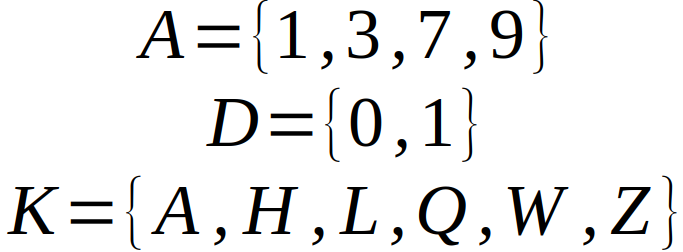
\includegraphics[width=40mm]{figures/sd_sets/enumeration_of_set.png}	
	\end{center}}    
\vspace{-4em}   	 
\end{frame}

\begin{frame}%задание множест2
	
	\begin{textitemize}	    
	\item с помощью определяющего высказывания, содержащего описание общего характеристического свойства, которым обладают все те и только те объекты, которые являются элементами (т.е. принадлежат) задаваемого множества.
    \end{textitemize}

\vspace{2em}

	\scnrelfrom{изображение}{
		
		\begin{center}
			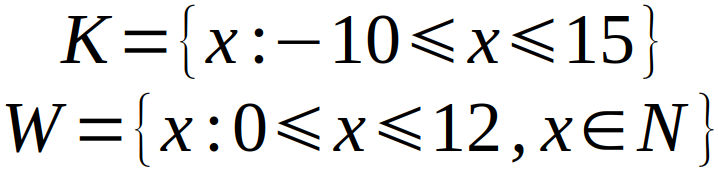
\includegraphics[width=45mm]{figures/sd_sets/descriptionProperties_set.png}
		\end{center}
	}
\vspace{-6em}      
\end{frame}

\begin{frame}%задание множест3
	
	\begin{textitemize}
	\item с помощью теоретико-множественных операций, позволяющих однозначно задавать новые множества на основе уже заданных (это операции объединения, пересечения, разности множеств и др.)
	\end{textitemize}

\vspace{2em}

    \scnrelfrom{изображение}{
     	
     	\begin{center}
     		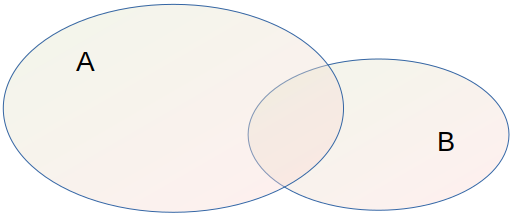
\includegraphics[width=40mm]{figures/sd_sets/unitiSets.png}
     	\end{center}
     }

\vspace{0.2em}
 
    \scnrelfrom{изображение}{
    	
    	\begin{center}
    		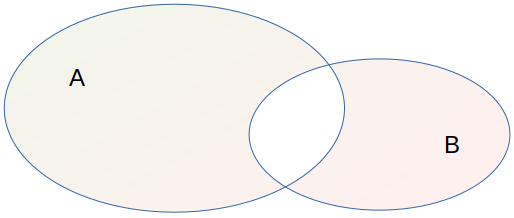
\includegraphics[width=40mm]{figures/sd_sets/intersectionSets.png}
    	\end{center}
    }

 
    
	\vspace{-4em}
\end{frame}

\begin{frame}{\\Принадлежность}
	\topline
	\justifying
	\begin{SCn}
		\scnheader{принадлежность*}
		\scnidtf{принадлежность элемента множеству*}
		\scniselement{бинарное отношение}
		\scniselement{ориентированное отношение}
	\end{SCn}
	
	\textbf{\textit{принадлежность*}} -- это бинарное ориентированное отношение, каждая связка которого связывает множество с одним из его элементов.\\
	\bigskip
	Элементами отношения \textbf{\textit{принадлежность*}} в \textit{SC-коде} по умолчанию являются \textbf{\textit{базовые sc-дуги}} (позитивные постоянные константные sc-дуги принадлежности).
\end{frame}

\begin{frame}{\\Классификация множеств}
	\topline
	\justifying
	\begin{SCn}
	\scnheader{множество}
	\begin{scnrelfromset}{разбиение}
		\scnitem{конечное множество}
		\scnitem{бесконечное множество}
	\end{scnrelfromset}
	\begin{scnrelfromset}{разбиение}
		\scnitem{множество без кратных элементов}
		\scnitem{мультимножество}
	\end{scnrelfromset}
	\begin{scnrelfromset}{разбиение}
		\scnitem{кортеж}
		\scnitem{неориентированное множество}
	\end{scnrelfromset}
	\end{SCn}
\end{frame}

\begin{frame}{\\Конечность множеств}
	\topline
	\justifying
	\begin{SCn}
	\scnheader{конечное множество}
	\scnidtf{множество с конечным числом элементов}
	\end{SCn}

	\textbf{\textit{конечное множество}} -- это \textit{множество}, количество элементов которого конечно, т.е. существует неотрицательное целое число \textit{k}, равное количеству элементов этого множества.
	\vspace{-\baselineskip}
	\begin{SCn}	
	\scnheader{бесконечное множество}
	\scnidtf{множество с бесконечным числом элементов}
	\begin{scnrelfromset}{разбиение}
		\scnitem{счетное множество}
		\scnitem{несчетное множество}
	\end{scnrelfromset}
	\end{SCn}
	\textbf{\textit{бесконечное множество}} -- это \textit{множество}, в котором для любого натурального числа \textit{n} найдётся конечное подмножество из \textit{n} элементов.

\end{frame}

\begin{frame}{\\Счетность множеств}
	\topline
	\justifying
	\textbf{\textit{счетное множество}} -- это \textit{бесконечное множество}, для которого существует \textit{взаимно однозначное соответствие} с натуральным рядом чисел.

	\begin{SCn}	
	\scnheader{несчетное множество}
	\scnidtf{континуальное множество}
	\end{SCn}

	\textbf{\textit{несчетное множество}} -- это \textit{бесконечное множество}, элементы которого невозможно пронумеровать натуральными числами.
\end{frame}

\begin{frame}{\\Кратность множеств}%множество без кратных элементов
	\topline
	\justifying
\begin{SCn}
	\scnheader{множество без кратных элементов}
	\scnidtf{классическое множество}
	\scnidtf{множество, состоящее из разных элементов}
	\scntext{пояснение}{\textbf{\textit{множество без кратных элементов}} -- это \textit{множество}, для каждого элемента которого существует только одна пара принадлежности, выходящая из знака этого множества в указанный элемент.}
\end{SCn}
\vspace{5.5em}
\end{frame}

\begin{frame}%мультимножество
	\topline
	\justifying
	
	\begin{SCn}	
		\scnheader{мультимножество}
		\scnidtf{множество, имеющее кратные вхождения хотя бы одного элемента}
		\scnidtf{множество, по крайней мере один элемент которого входит в его состав многократно}	
		\scntext{пояснение}{\textbf{\textit{мультимножество}} -- это \textit{множество}, для которого существует хотя бы одна кратная пара принадлежности, выходящая из знака этого множества.}
	\end{SCn}

\end{frame}
	
\begin{frame}%кратность принадлежности		
	\topline
	\justifying
	\vspace{10mm}
	\footnotesize
	\begin{SCn}
		\scnheader{кратность принадлежности}
		\scnidtf{кратность принадлежности элемента}
		\scnidtf{кратность вхождения элемента во множество}
		\scniselement{параметр}
		\scntext{пояснение}{\textbf{\textit{кратность принадлежности}} -- \textit{параметр}, значением которого являются числовые величины, показывающие сколько раз входит тот или иной элемент в рассматриваемое множество. Элементами данного параметра являются классы \textit{позитивных sc-дуг принадлежности}, связывающих данное множество с элементом, кратность вхождения которого в данное множество мы хотим задать. 

		Таким образом, кратное вхождение элемента в мультимножество может быть задано как явным указанием \textit{позитивных sc-дуг принадлежности} этого элемента данному \textit{множеству}, так и "склеиванием"{} этих дуг в одну и включением ее в некоторый класс \textbf{\textit{кратности принадлежности}}.}
	\end{SCn}

\vspace{6em}
\end{frame}

\begin{frame}%кратность принадлежности пример
\scnrelfrom{описание примера}{
	\begin{center}
	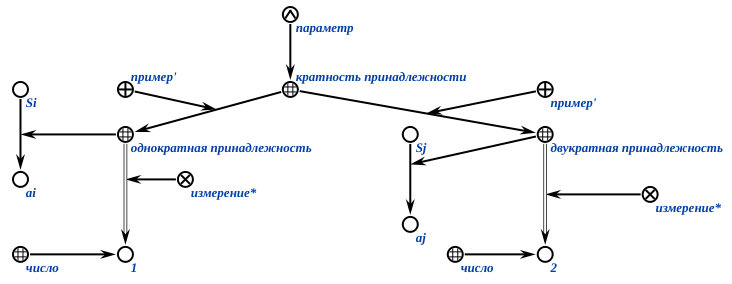
\includegraphics[width=120mm]{figures/sd_sets/multiplicityOfMembership.png}
	\end{center}
}
\vspace{-1em}
\end{frame}

\begin{frame}{\\Нечеткое и четкое множество }%нечеткое и четкое множество
\topline
\justifying
\vspace{10mm}
	\begin{SCn}		
\scnheader{нечеткое множество}
\scntext{пояснение}{\textbf{\textit{нечеткое множество}} -- это \textit{множество}, которое представляет собой совокупность элементов произвольной природы, относительно которых нельзя точно утверждать -- обладают ли эти элементы некоторым характеристическим свойством, которое используется для задания этого нечеткого множества. Принадлежность элементов такому множеству указывается при помощи \textit{нечетких позитивных sc-дуг принадлежности}.}

\scnheader{четкое множество}
\scntext{пояснение}{\textbf{\textit{четкое множество}} -- это \textit{множество}, принадлежность элементов которому достоверна и указывается при помощи \textit{четких позитивных sc-дуг принадлежности}.}
\end{SCn}

\end{frame}

\begin{frame}{\\Семейство множеств}%семейсво множеств 
	\topline
	\justifying
	\begin{SCn}
		\scnheader{семейство множеств}
		\scnidtf{множество множеств}
		\scnsuperset{класс классов}

	\scntext{пояснение}{\textbf{\textit{семейство множеств}} -- это \textit{множество}, элементами которого являются знаки множеств.}
		\end{SCn}
\vspace{8em}
\end{frame}

\begin{frame}{\\Свойства отношений на множестве}%свойства отношений на множестве 
	\topline
	\justifying
	
\begin{SCn}
\scnheader{нерефлексивное множество}
\scntext{пояснение}{\textbf{\textit{нерефлексивное множеств}} -- это \textit{множество}, знак которого не является элементом этого множества}

\scnheader{рефлексивное множество}
\scntext{пояснение}{\textbf{\textit{рефлексивное множеств}} -- это \textit{множество}, знак которого является элементом этого множества}
\end{SCn}

\vspace{-1em}
\end{frame}

\begin{frame}{\\Мощность}%мощность множества //невместилось 
	\topline
	\justifying
	
	\begin{SCn}
		\scnheader{мощность множества}
		\scnidtf{кардинальное число}
		\scnidtf{общее число вхождений элементов в заданное множество}
		\scnidtf{класс эквивалентности, элементами которого являются знаки всех тех и только тех множеств, которые имеют одинаковую мощность}
		\scnidtf{класс эквивалентности, соответствующий отношению быть парой множеств, имеющих одинаковую мощность (равномощность множеств)}
		\scnidtf{величина мощности множеств}
		\scnidtf{трансфинитное число}
		\scnidtf{мощность по Кантору}
		\scniselement{параметр}
	\end{SCn}
\end{frame}

\begin{frame}{\\Мощность}%мощность множества //невместилось 
	\topline
	\justifying
	\begin{SCn}
	\scnheader{мощность множества}
	\scntext{пояснение}{\textbf{\textit{мощность множества}} -- это \textit{параметр}, элементами которых являются \textit{множества}, имеющие одинаковое количество элементов. Значением данного параметра является числовая величина, задающая количество элементов, входящих в данный класс множеств, т.е. по сути, количество \textit{позитивных sc-дуг принадлежности}, выходящих из данного \textit{множества}.}
	
	\scnheader{множество}
	\scnsuperset{пустое множество}
	\scnsuperset{синглетон}
	\scnsuperset{пара}
	\scnsuperset{тройка}
	\end{SCn}
	\vspace{-2em}	
\end{frame}

\begin{frame}{\\Пустое множество} %пустое множество
  \topline
  \justifying
  
   \begin{SCn}
   	\scnheader{пустое множество}
   	\scniselement{мощность множества}
    \scntext{пояснение}{\textbf{\textit{пустое множество}} -- это \textit{множество}, которому не принадлежит ни один элемент.}
    \end{SCn}
    
\vspace{8.5em}
\end{frame}
    	
\begin{frame}{\\Синглетон}%синглетон 
	\topline
	\justifying
	
	\begin{SCn}
	\scnheader{синглетон}
	\scniselement{мощность множества}
	\scnidtf{множество мощности 1}
	\scnidtf{одноэлементное множество}
	\scnidtf{одномощное множество}
    \scnidtf{множество, мощность которого равна 1}
    \scnidtf{множество, имеющее мощность равную единице}
    \scnidtf{синглетон из sc-элемента} 
    \scnidtf{sc-синглеон}
    \scnsubset{конечное множество}
	\scntext{пояснение}{\textbf{\textit{синглетон}} -- это \textit{множество}, состоящее из одного элемента.}
	\end{SCn}
    	
\end{frame}

\begin{frame}{\\Пара}%пара
	\topline
\justifying
    \begin{SCn}
	\scnheader{пара}
	\scniselement{мощность множества}
	\scnidtf{множество мощности два}
	\scnidtf{двухэлементное множество}
	\scnidtf{двумощное множество}
	\scnsubset{конечное множество}
    \scntext{пояснение}{\textbf{\textit{пара}} -- это \textit{множество}, состоящее из двух элементов.}
    \end{SCn}
\vspace{4.5em} 	
    	
\end{frame}

\begin{frame}{\\Тройка} %тройка	
	\topline
\justifying
	
	\begin{SCn}
	\scnheader{тройка}
	\scniselement{мощность множества}
	\scnidtf{тройка}
	\scnidtf{множество мощности три}
	\scnsubset{конечное множество}
	\scntext{пояснение}{\textbf{\textit{тройка}} -- это \textit{множество}, состоящее из трех элементов.}
	\end{SCn}

\vspace{6em}
\end{frame}


	
\begin{frame}{\\Кортеж}%кортеж
	\topline
\justifying	
	
	\begin{SCn}
    \scnheader{кортеж}
    \scnidtf{вектор}
    \scntext{пояснение}{\textbf{\textit{кортеж}} -- это множество, представляющее собой упорядоченный набор элементов, т.е. такое множество, порядок элементов в котором имеет значение. Пары принадлежности элементов \textbf{\textit{кортежу}} могут дополнительно принадлежать каким-либо \textit{ролевым отношениям}, при этом, в рамках каждого \textbf{\textit{кортежа}} должен существовать хотя бы один элемент, роль которого дополнительно уточнена \textit{ролевым отношением}.}
	\end{SCn}

\vspace{2em}
\end{frame}

\begin{frame}
	\centering
	\Huge
	\textbf{Отношения на множествах}
\end{frame}

%%Отношения на множествах
\begin{frame}{\\Отношения на множествах}%включение
\topline
\justifying	
	\begin{SCn}
    \scnheader{включение*}
    \scnidtf{быть подмножеством*}
    \scniselement{бинарное отношение}
    \scniselement{ориентированное отношение}
    \scniselement{транзитивное отношение}
    \scnrelfrom{область определения}{множество}
    \scnsuperset{строгое включение*}
    \scntext{определение}{\textbf{\textit{включение*}} -- это бинарное ориентированное отношение, каждая связка которого связывает два множества. Будем говорить, что \textit{Множество Si} \textbf{\textit{включает*}} в себя \textit{Множество Sj} в том и только том случае, если каждый элемент \textit{Множества Sj} является также и элементом \textit{Множества Si}.}
	\end{SCn}
    \vspace{-3em}
\end{frame} 

\begin{frame}%рисунок включения
    \scnrelfrom{описание примера}{
    \begin{center}
    	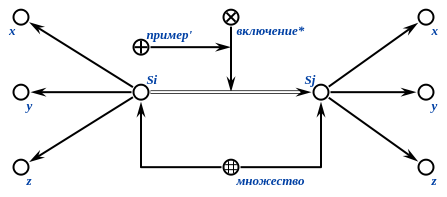
\includegraphics[width=100mm]{figures/sd_sets/inclusion.png}
    \end{center}}
    

    \begin{scnindent}
    \scntext{пояснение}{Множество \textbf{\textit{Sj}} включается во множество \textbf{\textit{Si}}.}
    \end{scnindent}
\vspace{-1em}
\end{frame}

\begin{frame}%строгое включение
	\topline
	\justifying	
	\vspace{10mm}
	\footnotesize
	\begin{SCn}
	\scnheader{строгое включение*}
	\scnidtf{строгое включение множеств*}
	\scnsubset{включение*}
	\scniselement{бинарное отношение}
	\scniselement{ориентированное отношение}
	\scnrelfrom{область определения}{множество}
    \scntext{определение}{\textbf{\textit{строгое включение*}} -- это \textit{бинарное ориентированное отношение}, областью определения которого является семейство всевозможных множеств. Будем говорить, что \textit{Множество Si} \textbf{\textit{строго включает*}} в себя \textit{Множество Sj} в том и только том случае, если каждый элемент \textit{Множество Sj} является также и элементом \textit{Множество Si}, при этом существует хотя бы один элемент \textit{Множество Si}, не являющийся элементом \textit{Множество Sj}.}
   	\end{SCn}
    \vspace{3em}
\end{frame}

\begin{frame}%рисунок строгое включение
	
    \scnrelfrom{описание примера}{
	\begin{center}
	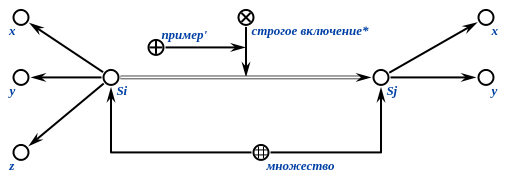
\includegraphics[width=22em]{figures/sd_sets/strictInclusion.png}
    \end{center}}
    
    \begin{scnindent}
    \scntext{пояснение}{Множество \textit{Sj} строго включается во множество \textit{Si}.}
    \end{scnindent}

\scnrelfrom{изображение}{
	\begin{center}
		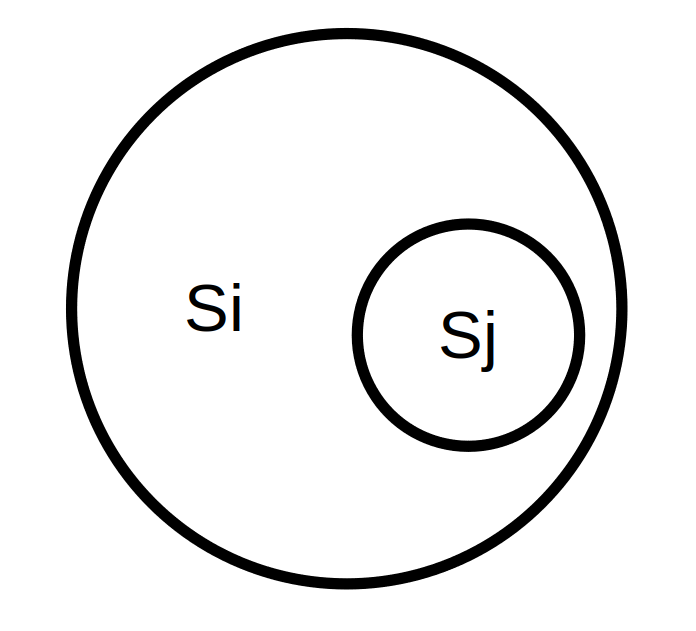
\includegraphics[width=7em]{figures/sd_sets/inclusion2.png}
\end{center}}

\vspace{-1.5em}
\end{frame}

\begin{frame}%равенство множеств
	\topline
	\justifying
	\vspace{10mm}
	
	\begin{SCn}
		\scnheader{равенство множеств*}
		\scniselement{бинарное отношение}
		\scniselement{неориентированное отношение}
		\scnidtf{быть равными множествами*}

	    \scntext{определение}{\textbf{\textit{равенство множеств}}* -- бинарное неориентированное отношение, выражающее отношение равенства множеств.
		Любые два множества являются равными множествами тогда и только тогда, когда первое является включением второго и второе является включением первого.}
	\end{SCn}
\vspace{9em}
\end{frame}

\begin{frame}%рисунок равенства множеств
    \scnrelfrom{описание примера}{
    \begin{center}
%не влазит
	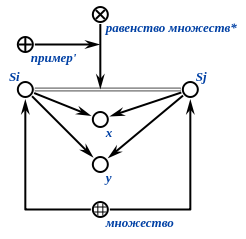
\includegraphics[width=50mm]{figures/sd_sets/equalityOfSets.png}
    \end{center}}

    \begin{scnindent}
    \scntext{пояснение}{Множество \textit{Si} равно множеству \textit{Sj}.}
    \end{scnindent}

\end{frame}

\begin{frame}%булеан
	\topline
	\justifying
	\vspace{5mm}
	\footnotesize
	
	\begin{SCn}
		\scnheader{булеан*}
		\scnidtf{булеан множества*}
		\scnidtf{семейство всевозможных подмножеств заданного множества*}
		\scniselement{бинарное отношение}
		\scniselement{ориентированное отношение}

    \scntext{определение}{\textbf{\textit{булеан*}} -- это \textit{бинарное ориентированное отношение} между множеством и некоторым семейством множеств, каждое из которых является подмножеством первого множества.}
    
    \scnrelfrom{описание примера}{
    \begin{center}
    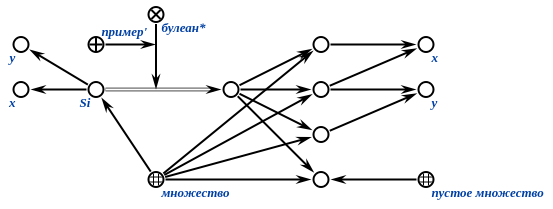
\includegraphics[width=100mm]{figures/sd_sets/boulean.png}
    \end{center}}
	\end{SCn}

\end{frame}

\begin{frame}%семейство подмножеств
\topline
\justifying
\vspace{5mm}
   \footnotesize
   \begin{SCn}
	\scnheader{семейство подмножеств*}
	\scnidtf{семейство подмножеств заданного множества*}
	\scniselement{бинарное отношение}
	\scniselement{ориентированное отношение}
	\scnsuperset{булеан*}

    \scntext{определение}{\textbf{\textit{семейство подмножеств*}} -- это \textit{бинарное ориентированное отношение} между множеством и некоторым семейством множеств, каждое из которых является подмножеством первого множества.}   
	
    \scnrelfrom{описание примера}{
    \begin{center}
    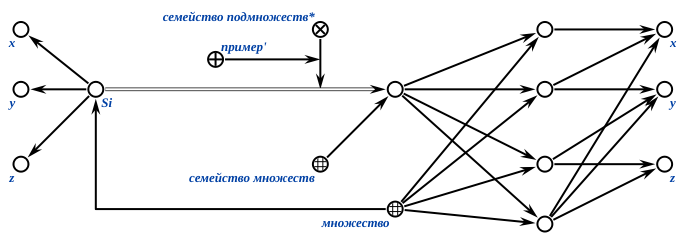
\includegraphics[width=100mm]{figures/sd_sets/familyOfSubsets.png}
    \end{center}}
	\end{SCn}

\end{frame}

%%Операции на множествах
\begin{frame}{\\Операции на множествах}%объединение
\topline
\justifying	
	\begin{SCn}
		\scnheader{объединение*}
		\scnidtf{объединение множеств*}
		\scniselement{квазибинарное отношение}
		\scniselement{ориентированное отношение}
	
    \scntext{определение}{\textbf{\textit{объединение*}} -- это \textit{квазибинарное ориентированное отношение}, областью определения которого является семейство всевозможных множеств. Будем говорить, что \textit{Множество Si} является объединением \textit{Множество Sj} и \textit{Множество Sk} тогда и только тогда, когда любой элемент \textit{Множество Si} является элементом или \textit{Множество Sj} или \textit{Множество Sk}.}
    \end{SCn}
    
    \vspace{1em}
   
\end{frame}

\begin{frame}%рисунок объединение	
 
  \scnrelfrom{описание примера}{
 	\begin{center}
 		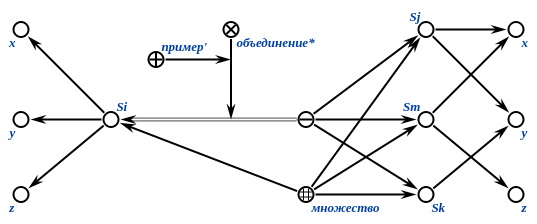
\includegraphics[width=75mm]{figures/sd_sets/union.png}
 \end{center}}
    \begin{scnindent}
    	\scntext{пояснение}{Множество \textit{Si} является объединением множеств \textit{Sj}, \textit{Sk} и \textit{Sm}.}
    \end{scnindent}

    \scnrelfrom{изображение}{
    \begin{center}
    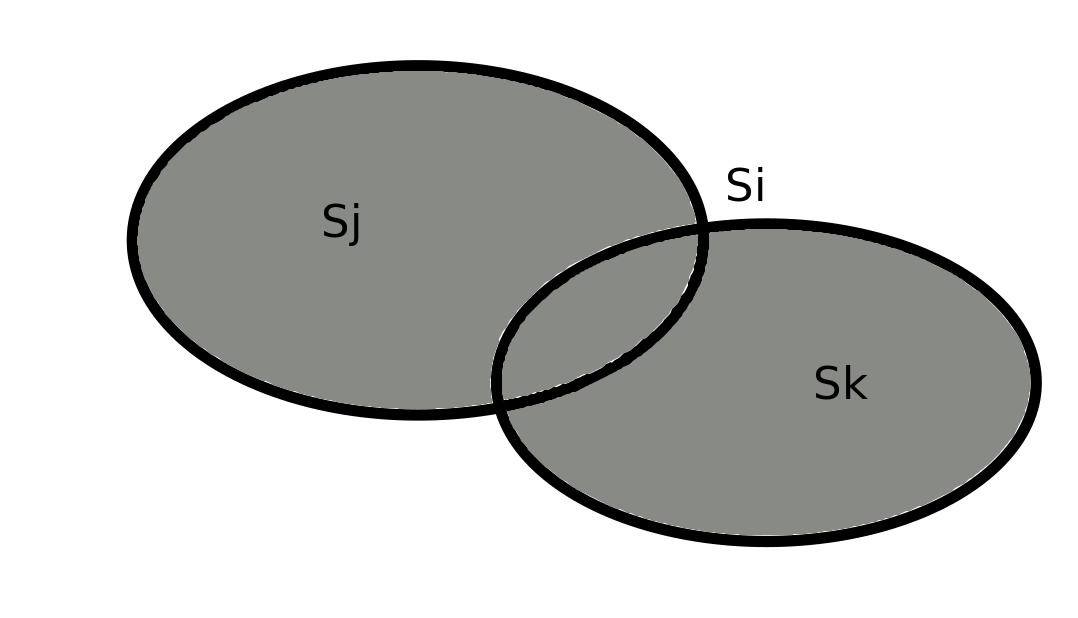
\includegraphics[width=45mm]{figures/sd_sets/union2.png}
    \end{center}}
\vspace{-3em}
\end{frame}

%%еще не сделано ошибка
\begin{frame}%разбиение 
\topline
\justifying

	\begin{SCn}
	\scnheader{разбиение*}
	\scnidtf{разбиение  множества*}
	\scnidtf{объединение попарно непересекающихся множеств*}
	\scnidtf{декомпозиция множества*}
	\scniselement{квазибинарное отношение}
	\scniselement{ориентированное отношение}
	\scniselement{отношение декомпозиции}
	\end{SCn}
\end{frame}

\begin{frame}
\topline
\justifying
\vspace{10mm}	
\footnotesize
	\begin{SCn}
	\scnheader{разбиение*}
\scntext{определение}{\textbf{\textit{разбиение*}} -- это \textit{квазибинарное ориентированное отношение}, областью определения которого является семейство всевозможных множеств. В результате разбиения множества получается множество попарно непересекающихся множеств, объединение которых есть исходное множество.
	
	Семейство множеств \{\textit{S1…, Sn}\} является разбиением множества \textit{Si} в том и только том случае, если:

	\begin{textitemize}
		\item семейство \{\textit{S1…, Sn}\} является семейством \textit{попарно непересекающихся множеств};
		\item семейство \{\textit{S1…, Sn}\} является покрытием множества \textit{Si} (множество \textit{Si} является \textit{объединением} множеств, входящих в указанное выше семейство)
	\end{textitemize}}
\end{SCn}
\end{frame}

\begin{frame}%разбиение2 + рисунок
	    
    \scnrelfrom{описание примера}{
    \begin{center}
    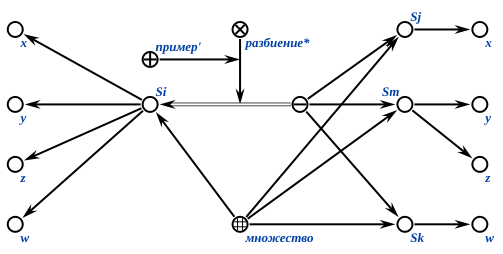
\includegraphics[width=60mm]{figures/sd_sets/split.png}
    \end{center}}

    \begin{scnindent}
    \scntext{пояснение}{Множество \textit{Si} разбивается на множества \textit{Sj}, \textit{Sk} и \textit{Sm}.}
    \end{scnindent}

    \scnrelfrom{изображение}{
    \begin{center}
	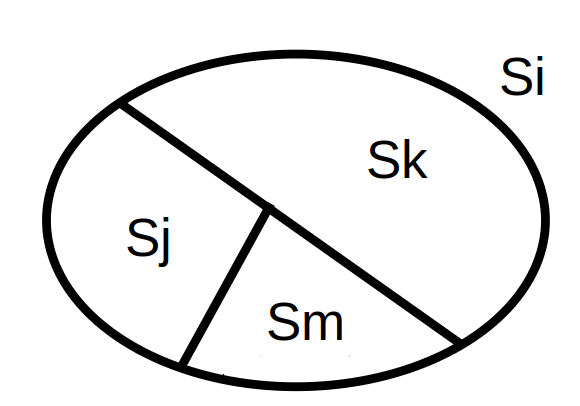
\includegraphics[width=40mm]{figures/sd_sets/split2.png}
    \end{center}}

\end{frame}

\begin{frame}%пересечение
\topline
\justifying
\vspace{10mm}

	\begin{SCn}
	\scnheader{пересечение*}
	\scnidtf{пересечение множеств*}
	\scniselement{квазибинарное отношение}
	\scniselement{ориентированное отношение}
	\end{SCn}
    
    \scntext{определение}{\textbf{\textit{пересечение*}} -- это операция над множествами, аргументами которой являются два или большее число множеств, а результатом является множество, элементами которого являются все те и только те сущности, которые одновременно принадлежат каждому множеству, которое входит в семейство аргументов этой операции.\\
	Будем говорить, что \textit{Множество Si} является пересечением \textit{Множество Sj} и \textit{Множество Sk} тогда и только тогда, когда любой элемент \textit{Множество Si} является элементом \textit{Множество Sj} и элементом \textit{Множество Sk}.}
\vspace{6em}
\end{frame}

\begin{frame}%пересечение рисунки
	
    \scnrelfrom{описание примера}{
    \begin{center}
	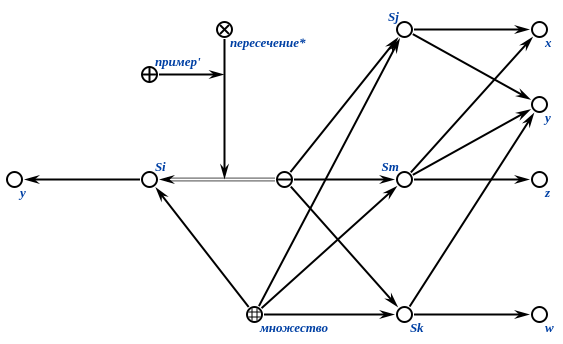
\includegraphics[width=70mm]{figures/sd_sets/intersection.png}
    \end{center}}

    \begin{scnindent}
    \scntext{пояснение}{Множество \textit{Si} является результатом пересечения множеств \textit{Sj}, \textit{Sk} и \textit{Sm}.}
    \end{scnindent}

    \scnrelfrom{изображение}{
    \begin{center}
	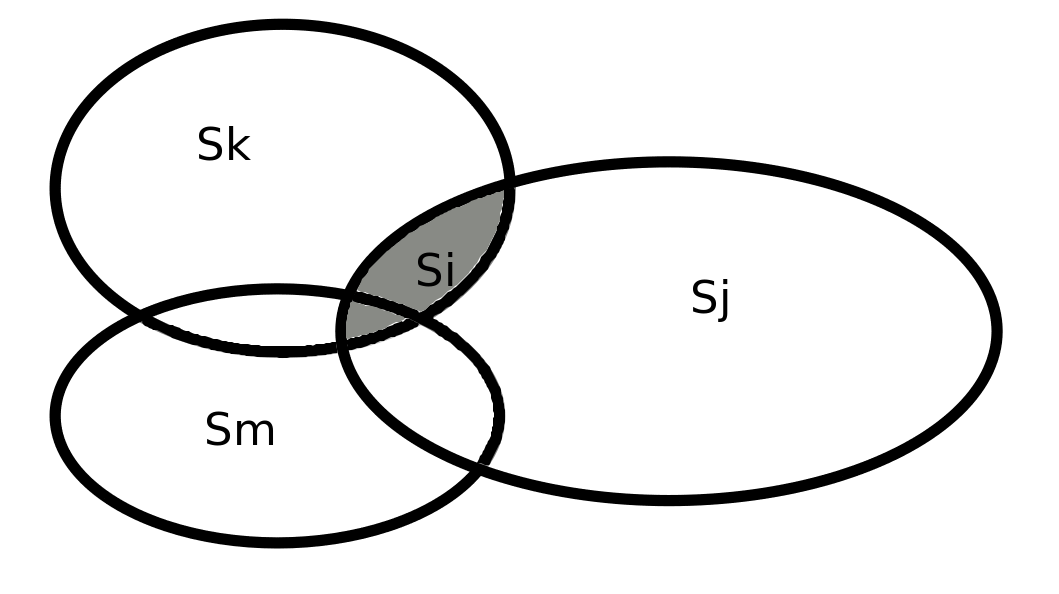
\includegraphics[width=40mm]{figures/sd_sets/intersection2.png}
    \end{center}} 

\end{frame}

\begin{frame}%разность
\topline
\justifying
\vspace{10mm}	

	\begin{SCn}
	\scnheader{разность множеств*}
	\scniselement{бинарное отношение}
	\scniselement{ориентированное отношение}
	\scntext{определение}{\textbf{\textit{разность множеств*}} -- это \textit{бинарное ориентированное отношение}, связывающее между собой \textit{ориентированную пару}, первым элементом которой является уменьшаемое множество, вторым -- вычитаемое множество, и множество, являющееся результатом вычитания вычитаемого из уменьшаемого, в которое входят все элементы первого множества, не входящие во второе множество.}
	\end{SCn}
   
  \vspace{10em} 
\end{frame}   

\begin{frame}%разность рисунок 

   \scnrelfrom{описание примера}{
   \begin{center}
   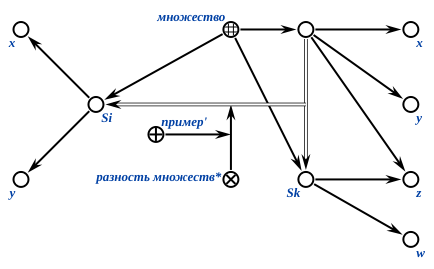
\includegraphics[width=75mm]{figures/sd_sets/setDifference.png}
   \end{center}}

   \begin{scnindent}
   \scntext{пояснение}{Множество \textit{Si} является результатом разности множеств \textit{Sj} и \textit{Sk}.}
   \end{scnindent}

   \scnrelfrom{изображение}{
   \begin{center}
   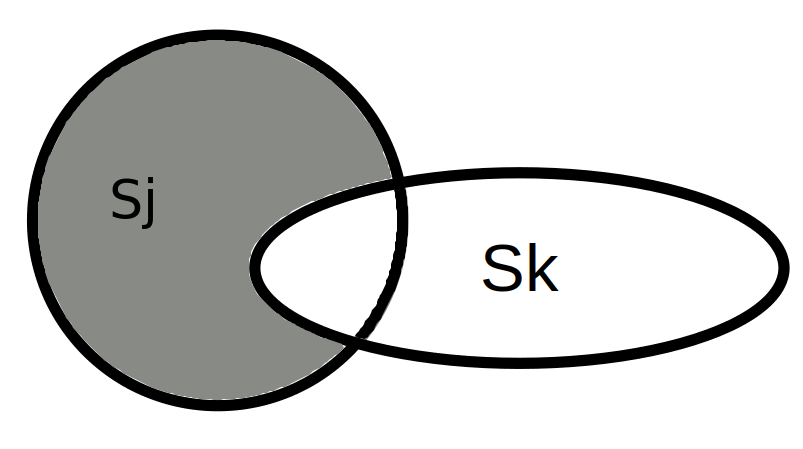
\includegraphics[width=40mm]{figures/sd_sets/setDifference2.png}
   \end{center}}

\end{frame}

\begin{frame}%сим.разность
\topline
\justifying
\vspace{10mm}	

	\begin{SCn}
	\scnheader{симметрическая разность множеств*}
	\scniselement{бинарное отношение}
	\scniselement{ориентированное отношение}

    \scntext{определение}{\textbf{\textit{симметрическая разность множеств*}} -- это \textit{бинарное ориентированное отношение}, связывающее между собой \textit{пару} множеств и множество, являющееся результатом симметрической разности элементов указанной пары. Будем называть \textit{Множество Si} результатом симметрической разности \textit{Множества Sj} и \textit{Множества Sk} тогда и только тогда, когда любой элемент \textit{Множества Si} является или элементом \textit{Множества Sj} или \textit{Множества Sk}, но не является элементом обоих множеств.}
	\end{SCn}
\vspace{8em}
\end{frame}

\begin{frame}%сим.разность рис
	
    \scnrelfrom{описание примера}{
    \begin{center}
	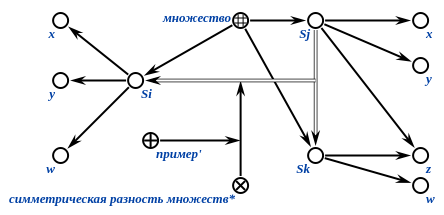
\includegraphics[width=75mm]{figures/sd_sets/symmetricDifferenceOfSets.png}
	\end{center}}

	\scntext{пояснение}{Множество \textit{Si} является результатом симметрической разности множеств \textit{Sj} и \textit{Sk}.}
	
    \scnrelfrom{изображение}{
    \begin{center}
	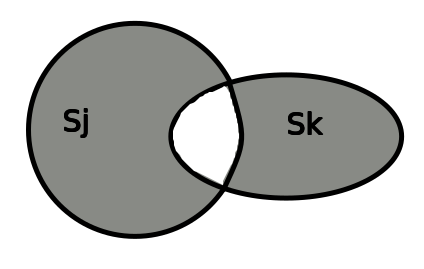
\includegraphics[width=35mm]{figures/sd_sets/symmetricDifferenceOfSets2.png}
    \end{center}}

\end{frame}

\begin{frame}%декартово произведение
\topline
\justifying
\vspace{10mm}	
	
	\begin{SCn}
	\scnheader{декартово произведение*}
	\scnidtf{декартово произведение множеств*}
	\scnidtf{прямое произведение множеств*}
	\scniselement{бинарное отношение}
	\scniselement{ориентированное отношение}
    \scntext{определение}{\textbf{\textit{декартово произведение*}} -- это \textit{бинарное ориентированное отношение} между \textit{ориентированной парой} множеств и \textit{множеством}, элементами которого являются всевозможные упорядоченные пары, первыми элементами которых являются элементы первого из указанных множеств, вторыми -- элементы второго из указанных множеств.}
	\end{SCn}

\vspace{10em}
\end{frame}

\begin{frame}%декартово произведение рис
	
    \scnrelfrom{описание примера}{
    \begin{center}
	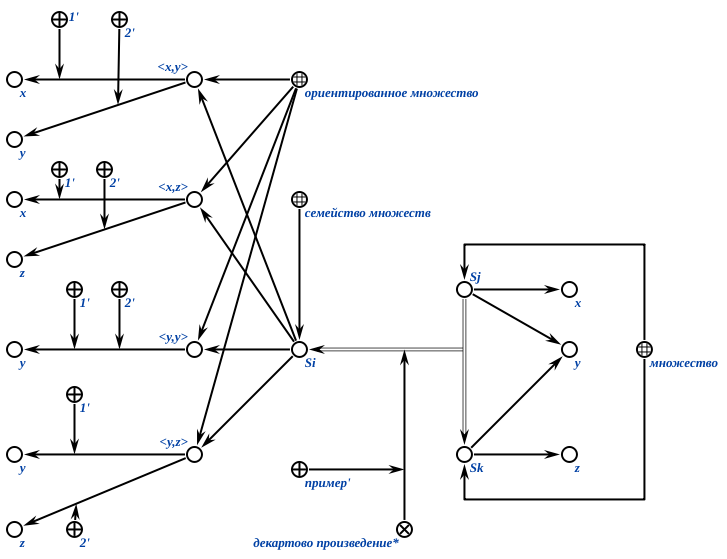
\includegraphics[width=80mm]{figures/sd_sets/cartesianMultiplication.png}
    \end{center}}

    \begin{scnindent}
    \scntext{пояснение}{Множество \textit{Si} является результатом декартова произведения множеств \textit{Sj} и \textit{Sk}.}
    \end{scnindent}

\end{frame}

%Пересекающиеся множества
\begin{frame}{\\Пересекающиеся множества}%пара пересек.множ.
\topline
\justifying	
	\begin{SCn}
	\scnheader{пара пересекающихся множеств*}
    \scniselement{бинарное отношение}
    \scniselement{неориентированное отношение}
    
	\scntext{пояснение}{\textbf{\textit{пара пересекающихся множеств*}} -- \textit{бинарное неориентированное отношение} между двумя \textit{множествами}, имеющими непустое \textit{пересечение*}.} 
   
	\scntext{определение}{\textbf{\textit{пара пересекающихся множеств*}} -- \textit{бинарное неориентированное отношение} между двумя \textit{множествами}, имеющими, по крайней мере, один общий для этих двух множеств элемент.}
	\end{SCn}
\vspace{1em}
\end{frame}
 
\begin{frame}%пара пересек.множ.рис.

   \scnrelfrom{описание примера}{
   \begin{center}
   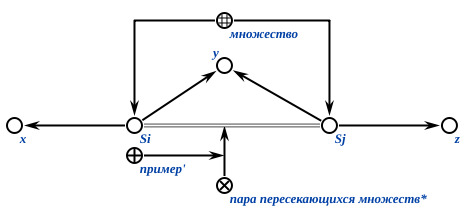
\includegraphics[width=80mm]{figures/sd_sets/pairOfIntersectingSets.png}
   \end{center}}

   \begin{scnindent}
   \scntext{пояснение}{Множество \textit{Si} и множество \textit{Sj} являются парой пересекающихся множеств.}
   \end{scnindent}
   
   \scnrelfrom{изображение}{
   \begin{center}	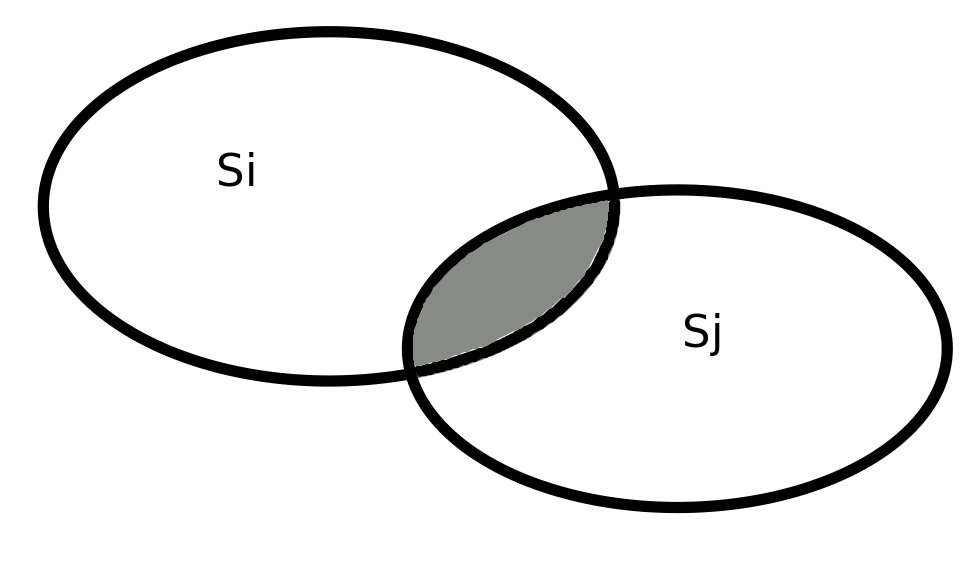
\includegraphics[width=40mm]{figures/sd_sets/pairOfIntersectingSets2.png}
   \end{center}}
\vspace{-2em}
\end{frame}

\begin{frame}%попарно пересек.множ.
\topline
\justifying
\vspace{10mm}	
	
	\begin{SCn}
	\scnheader{попарно пересекающиеся множества*}
	\scnidtf{семейство попарно пересекающихся множеств*}
	\scnsuperset{пересекающиеся множества*}
	\scniselement{отношение}

    \scntext{определение}{\textbf{\textit{попарно пересекающиеся множества*}} -- семейство множеств, каждая пара которых является парой пересекающихся множеств, т.е. каждая пара которых имеет хотя бы один общий элемент}
    
    \scntext{примечание}{Не каждое \textit{семейство попарно пересекающихся множеств*} является \textit{семейством пересекающихся множеств*}, хотя обратное верно.}
	\end{SCn}   
  
\vspace{9em}
\end{frame}

\begin{frame}%попарно пресек.множ.рис.%не влезло
	    
      \scnrelfrom{изображение}{
    	\begin{center}
    		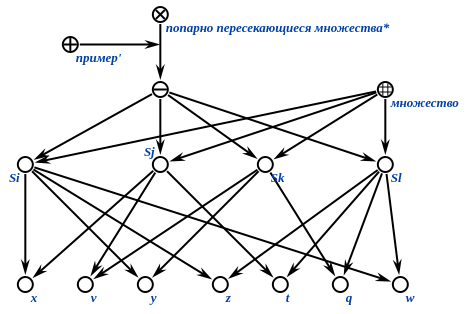
\includegraphics[width=50mm]{figures/sd_sets/pairwiseIntersectingSets.png}
  \end{center}}

   \begin{scnindent}
   \scntext{пояснение}{Множества \textit{Si}, \textit{Sj}, \textit{Sk} и \textit{Sl} являются попарно пересекающимися множествами.}
   \end{scnindent}


   \scnrelfrom{изображение}{
   \begin{center}
   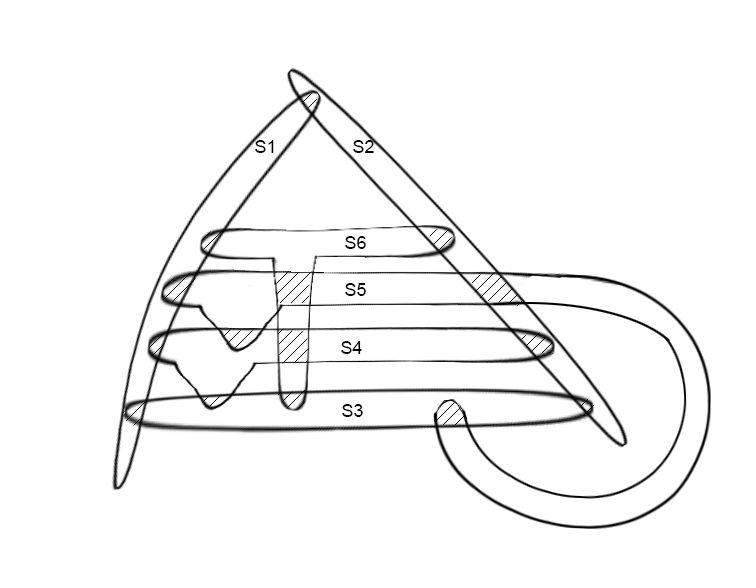
\includegraphics[width=40mm]{figures/sd_sets/pairwiseIntersectingSets2.png}
   \end{center}}

\end{frame}

\begin{frame}%пересекающиеся множества
\topline
\justifying
\vspace{10mm}
	
	\begin{SCn}
    \scnheader{пересекающиеся множества*}
    \scnidtf{семейство пересекающихся множеств*}
    \scnidtf{быть семейством пересекающихся множеств*}
    \scnidtf{семейство множеств, имеющих по крайней мере один элемент, являющийся общим для всех этих множеств*}
    \scnsuperset{попарно пересекающиеся множества*}

    \scntext{определение}{\textbf{\textit{пересекающиеся множества*}} -- это семейство множеств, имеющих по крайней мере один общий для всех этих множеств элемент}
    \end{SCn}
   
\vspace{14em}
\end{frame}

\begin{frame}%пересекающиеся множества рис.

   \scnrelfrom{описание примера}{
  	\begin{center}
  		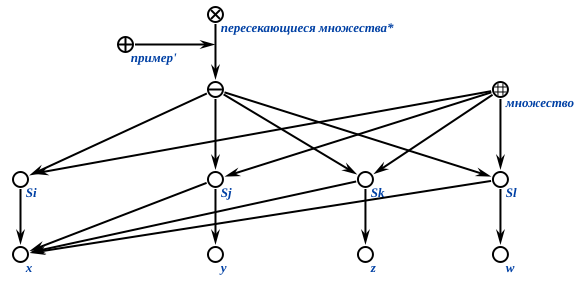
\includegraphics[width=100mm]{figures/sd_sets/intersectingSets.png}
  \end{center}}
  \begin{scnindent}
  	\scntext{пояснение}{Множества \textit{Si}, \textit{Sj}, \textit{Sk} и \textit{Sl} являются пересекающимися множествами.}
  \end{scnindent}
\vspace{2em}
\end{frame}

\begin{frame}%пара непересек.множ.
\topline
\justifying
\vspace{10mm}	
	
	\begin{SCn}
    \scnheader{пара непересекающихся множеств*}
    \scniselement{бинарное отношение}
    \scniselement{неориентированное отношение}
    
    \scntext{определение}{\textbf{\textit{пара непересекающихся множеств*}} -- это \textit{бинарное неориентированное отношение} между \textit{множествами}, результатом \textit{пересечения*} которых есть пустое множество.}
	\end{SCn}
  
\vspace{15em}
\end{frame}

\begin{frame}%пара непересек.множ.рис.
	
       \scnrelfrom{описание примера}{
   	\begin{center}
   		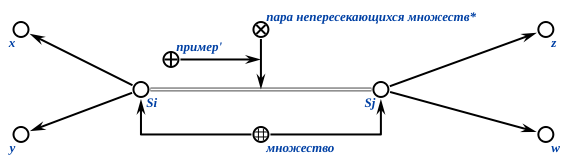
\includegraphics[width=90mm]{figures/sd_sets/pairOfNonIntersectingSets.png}
   \end{center}}
   
   
   \begin{scnindent}
   	\scntext{пояснение}{Множества \textit{Si} и \textit{Sj} являются парой непересекающихся множеств.}
   \end{scnindent}
   
   \scnrelfrom{изображение}{
   	\begin{center}
   		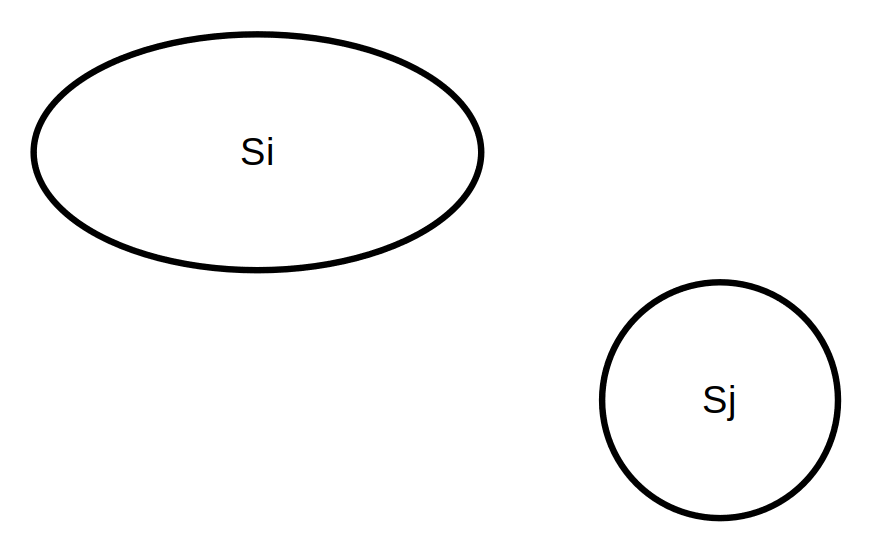
\includegraphics[width=40mm]{figures/sd_sets/pairOfNonIntersectingSets2.png}
   \end{center}} 

    

\end{frame}

\begin{frame}%попарно непересек.множ.
\topline
\justifying
\vspace{10mm}

	\begin{SCn}
	\scnheader{попарно непересекающиеся множества*}
    \scnidtf{семейство попарно непересекающихся множеств*}
    \scnsubset{непересекающиеся множества*}
    \scntext{определение}{\textbf{\textit{попарно непересекающиеся множества*}} -- семейство множеств, каждая пара которых является парой непересекающихся множеств, т.е. каждая пара которых не имеет ни одного общего элемента}
	\end{SCn}

    \vspace{15em}
\end{frame}

\begin{frame}%попарно непересек.множ.рис.    
    \scnrelfrom{изображение}{
    \begin{center}	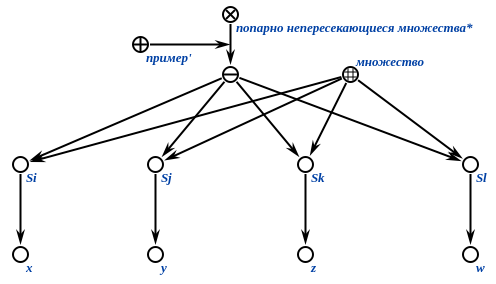
\includegraphics[width=90mm]{figures/sd_sets/pairwiseNonIntersectingSets.png}
    \end{center}}

    \begin{scnindent}
    \scntext{пояснение}{Множества \textit{Si}, \textit{Sj}, \textit{Sk} и \textit{Sl} являются попарно непересекающимися множествами.}
    \end{scnindent}

\end{frame}

\begin{frame}%непересек.множ.
\topline
\justifying
\vspace{10mm}	

	\begin{SCn}
    \scnheader{непересекающиеся множества*}
    \scnidtf{семейство непересекающихся множеств*}
    \scnidtf{быть семейством непересекающихся множеств*}
    \scntext{определение}{\textbf{\textit{непересекающиеся множества*}} -- это семейство множеств, не имеющих ни одного общего элемента для всех этих множеств}
	\end{SCn}

    \vspace{15em}
\end{frame}

\begin{frame}    
    \scnrelfrom{изображение}{
    \begin{center}
  	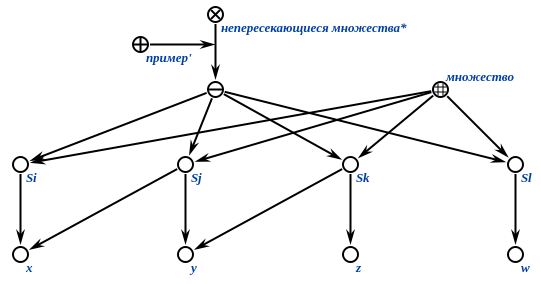
\includegraphics[width=90mm]{figures/sd_sets/nonIntersectingSets.png}
    \end{center}}

 	\scntext{пояснение}{Множества \textit{Si}, \textit{Sj}, \textit{Sk} и \textit{Sl} являются непересекающимися множествами.}

\end{frame}

\title{Лекция 6\\Представление в базе знаний отношений и их свойств}   
\author[]{Шункевич Д.В.}
\institute[]{Белорусский государственный университет информатики и радиоэлектроники}

\begin{frame}
	\titlepage
\end{frame}

\begin{frame}{\\Содержание лекции}
	\topline
	\justifying
	Бинарное отношение и способы его задания. Рефлексивное и арефлексивное бинарное отношение. Симметричное и антисимметричное бинарное отношение. Транзитивное бинарное отношение. Отношения строгого и нестрогого порядка. Отношения полного (линейного) и частичного порядка. Отношения эквивалентности и толерантности. Квазибинарное отношение. n-арное отношение, схема отношения. Область определения отношения, домен. Операции над отношениями (проекция, соединение, композиция). Метаотношения, примеры. Представление в базе знаний.
\end{frame}
\title{Лекция 7\\Представление в базе знаний параметров и величин}   
\author[]{Шункевич Д.В.}
\institute[]{Белорусский государственный университет информатики и радиоэлектроники}

\begin{frame}
	\titlepage
\end{frame}

\begin{frame}{\\Содержание лекции}
	\topline
	\justifying
	Понятие шкалы, величины и параметра. Измеряемые и неизмеряемые параметры. Точные, неточные и интервальные величины. Связь с понятием мощности множества, бесконечного и конечного множества.
\end{frame}
\title{Лекция 8\\Представление структур и семантических окрестностей в базе знаний}   
\author[]{Шункевич Д.В.}
\institute[]{Белорусский государственный университет информатики и радиоэлектроники}

\begin{frame}
	\titlepage
\end{frame}

\begin{frame}{\\Содержание лекции}
	\topline
	\justifying
	Понятие структуры как фрагмента базы знаний. Типология структур, роли элементов структуры. Отношения на структурах. Представление в базе знаний метаинформационных конструкций. Понятие семантической окрестности, типология семантических окрестностей.
\end{frame}

\begin{frame}{Понятие структуры как фрагмента базы знаний}
	\topline
	\justifying
	При накоплении больших	объемов информации в базе знаний возникает необходимость выделять \textbf{целые фрагменты} базы знаний и иметь возможность их специфицировать, рассматривая \textbf{как отдельные сущности}.\\
	Такой фрагмент базы знаний назван структурой (sc-структурой).\\
	Под \textbf{структурой} будем понимать \textbf{множество
	sc-элементов}, удаление одного из которых может привести к нарушению целостности этого множества.
\end{frame}

\begin{frame}{**}
	\topline
	\justifying
	Структура может изображаться путем явного указания всех пар принадлежности элементов этой структуре, а также в виде контура, содержащего все элементы, входящие в состав этой структуры.
\end{frame}

\begin{frame}{Пример представления структуры как фрагмента базы знаний}
	\topline
	\justifying
	\begin{figure}[H]
		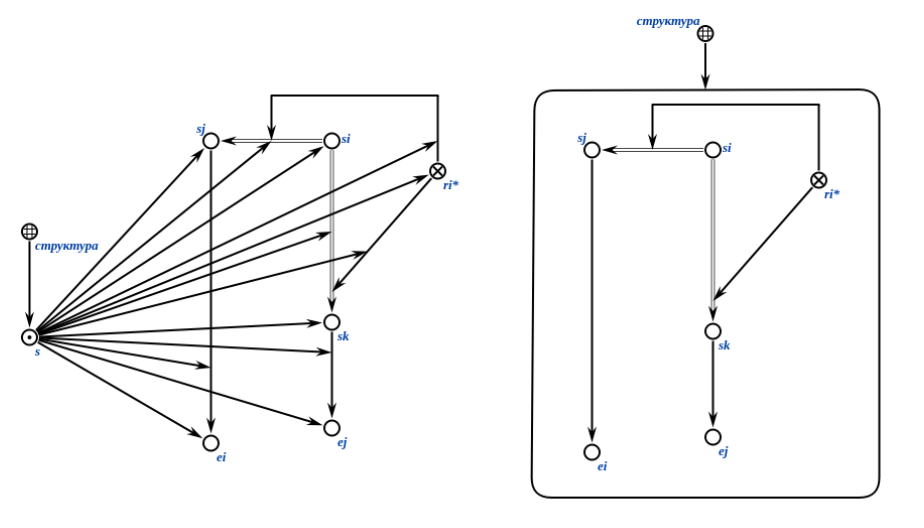
\includegraphics[scale=0.33]{./figures/sd_structures/structure.png}
	\end{figure}
\end{frame}

\begin{frame}{\\Типология структур}
	\topline
	\justifying
	\scnheader{структура}
	\begin{scnrelfromset}{разбиение}
		\scnitem{связная структура}
		\scnitem{несвязная структура}
	\end{scnrelfromset}
	\begin{scnrelfromset}{разбиение}
		\scnitem{тривиальная структура}
		\begin{scnindent}
			\scnidtf{структура, не содержащая связок}
		\end{scnindent}
		\scnitem{нетривиальная структура}
		\begin{scnindent}
			\scnidtf{структура, содержащая хотя бы одну связку}
		\end{scnindent}
	\end{scnrelfromset}
\end{frame}


\begin{frame}{\\Типология структур}
	\topline
	\justifying
	Структуре, представленной в SC-коде, поставим в соответствие орграф, вершинами которого являются sc-элементы, а дугами – связки отношений инцидентности, связывающие sc-коннекторы с инцидентными им sc-элементами, которые являются компонентами указанных sc-коннекторов. Если полученный таким способом орграф является связным орграфом, то исходную структуру будем считать связной структурой.\\ Если полученный	таким способом орграф не является связным орграфом, то исходную структуру будем считать несвязной структурой.
\end{frame}


\begin{frame}{\\Типология структур}
	\topline
	\justifying
	
	По признаку стационарности выделяются динамические структуры (процессы),	состав которых меняется с течением времени, и статические структуры, состав которых не меняется	с течением времени.
	\scnheader{структура}
	\begin{scnrelfromset}{разбиение}
		\scnitem{процесс}
		\begin{scnindent}
			\scnidtf{динамическая структура}
			\scnidtf{нестационарная структура}
		\end{scnindent}
		\scnitem{статическая структура}
		\begin{scnindent}
			\scnidtf{стационарная структура}
			\scnidtf{структура, не изменяющаяся во времени}
		\end{scnindent}
	\end{scnrelfromset}
\end{frame}

\begin{frame}{\\Типология структур}
	\topline
	\justifying
	
	По признаку времени существования выделяются временные структуры и постоянно существующие структуры.
	\scnheader{структура}
	\begin{scnrelfromset}{разбиение}
		\scnitem{временная структура}
		\scnitem{постоянно существующая структура}
	\end{scnrelfromset}
\end{frame}

\begin{frame}{\\Роли элементов структуры}
	\topline
	\justifying
	
	Для формального представления структур используются понятия, описывающие роли элементов в рамках структуры. Элемент структуры\scnrolesign – неосновное понятие, ролевое отношение, указывающее на все элементы каждой структуры.
	\scnheader{элемент структуры\scnrolesign}
	\begin{scnrelfromset}{разбиение}
		\scnitem{непредставленное множество\scnrolesign}
		\scnitem{полностью представленное множество\scnrolesign}
		\scnitem{частично представленное множество\scnrolesign}
		\scnitem{элемент структуры, не являющийся множеством\scnrolesign}
	\end{scnrelfromset}
\end{frame}

\begin{frame}{\\Роли элементов структуры}
	\topline
	\justifying
	
	\scnheader{элемент структуры\scnrolesign}
	\begin{scnrelfromset}{разбиение}
		\scnitem{максимальное множество\scnrolesign}
		\begin{scnindent}
			\scnrelfrom{пояснение}{Ролевое отношение, связывающее структуру со знаком множества, для которого не существует множества, которое было бы надмножеством указанного множества и знак которого был бы элементом этой же структуры}
		\end{scnindent}
		\scnitem{немаксимальное множество\scnrolesign}
		\begin{scnindent}
			\scnrelfrom{пояснение}{Ролевое отношение, связывающее структуру со знаком множества, для которого в рамках данной структуры существует множество, являющееся надмножеством указанного множества.}
		\end{scnindent}
	\end{scnrelfromset}
\end{frame}

\begin{frame}{\\Роли элементов структуры}
	\topline
	\justifying
	
	\scnheader{элемент структуры\scnrolesign}
	\begin{scnrelfromset}{разбиение}
		\scnitem{первичный элемент\scnrolesign}
		\begin{scnindent}
			\scnrelfrom{пояснение}{Ролевое отношение, указывающее на (атомарный) элемент структуры, который не имеет элементов, ему принадлежащих. При этом	соответствующая пара принадлежности может существовать, но в состав данной структуры не входить.}
		\end{scnindent}
		\scnitem{вторичный элемент\scnrolesign}
		\begin{scnindent}
			\scnrelfrom{пояснение}{Ролевое отношение, указывающее на элемент структуры, обозначающий множество элементов, где обязательно хотя бы один элемент указанного множества входил бы в указанную структуру.}
		\end{scnindent}
	\end{scnrelfromset}
\end{frame}

\begin{frame}{\\Роли элементов структуры}
	\topline
	\justifying
	
	\scnheader{элемент структуры\scnrolesign}
	\begin{scnrelfromset}{разбиение}
		\scnitem{элемент первого уровня\scnrolesign}
		\begin{scnindent}
			\scnrelfrom{пояснение}{связка первичных элементов, тривиальная структура из первичных элементов или класс первичных элементов}
		\end{scnindent}
		\scnitem{структура второго уровня\scnrolesign}
		\begin{scnindent}
			\scnrelfrom{пояснение}{структура, среди элементов которой есть хотя бы один элемент второго уровня\scnrolesign}
		\end{scnindent}
	\end{scnrelfromset}
\end{frame}

\begin{frame}{\\Пример ролей элементов структуры}
	\topline
	\justifying
	\begin{figure}[H]
		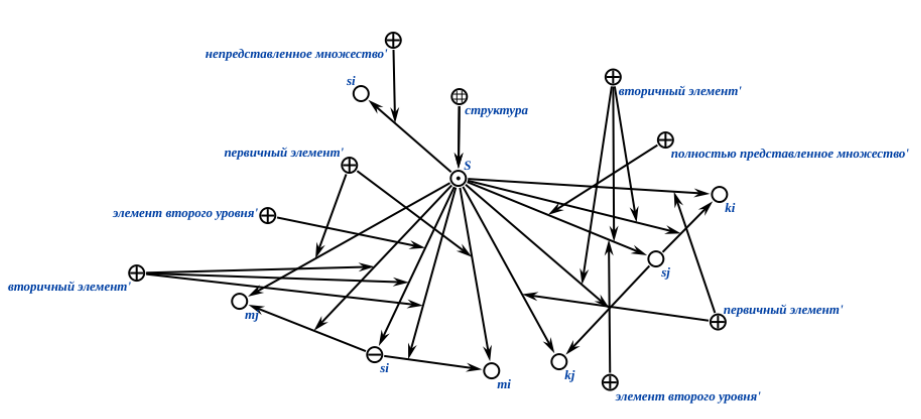
\includegraphics[scale=0.37]{./figures/sd_structures/roles.png}
	\end{figure}
\end{frame}

\begin{frame}{\\Отношения на структурах}
	\topline
	\justifying
	\scnheader{бинарное отношение*}
	\scnhaselement{полиморфность* }
		\begin{scnindent}
			\scnsubset{соответствие*}
		\end{scnindent}
	\scnhaselement{полиморфизм*}
	\scnhaselement{гомоморфность*}
		\begin{scnindent}
		\scnsubset{соответствие*}
		\end{scnindent}
	\scnhaselement{гомоморфизм*}
	\scnhaselement{изоморфность*}
		\begin{scnindent}
		\scnsubset{соответствие*}
		\end{scnindent}
	\scnhaselement{изоморфизм*}
	\scnhaselement{автомоморфность*}
		\begin{scnindent}
		\scnsubset{соответствие*}
		\end{scnindent}
	\scnhaselement{автоморфизм*}
\end{frame}

\begin{frame}{\\Отношения на структурах}
	\topline
	\justifying
	
	\scnheader{полиморфность* }
	\scnrelfrom{пояснение}{полиморфность* - это соответствие, заданное на структурах, при котором каждому элементу из области	определения соответствия (первой структуры) ставится в соответствие один или более элемент из областизначения соответствия (второй структуры), при этом существует хотя бы один элемент области определения	соответствия, которому соответствуют два или более элемента из области значения соответствия.}
\end{frame}

\begin{frame}{\\Отношения на структурах}
	\topline
	\justifying
	
	\scnheader{гомоморфность*}
	\scnrelfrom{пояснение}{гомоморфность* - это соответствие, заданное на структурах, при котором каждому элементу из области	определения соответствия (первой структуры) ставится в соответствие только один элемент из области		значения соответствия (второй структуры).}
\end{frame}

\begin{frame}{\\Отношения на структурах}
	\topline
	\justifying
	
	\scnheader{изоморфность*}
	\scnrelfrom{пояснение}{изоморфность* - это гомоморфность*, при которой для каждого элемента из области значения существует	ровно один соответствующий элемент из области определения.}
	
	
	\scnheader{автомоморфность*}
	\scnrelfrom{пояснение}{автоморфность* - это изоморфность*, у которой область определения соответствия и область значения соответствия совпадают.}
\end{frame}

\begin{frame}{\\Отношения на структурах}
	\topline
	\justifying
	
	\scnheader{аналогичность структур*}
	\scnsubset{соответствие*}
	\scniselement{бинарное отношение*}
	\scnrelfrom{пояснение}{аналогичность структур* - соответствие*, задаваемое на структурах, и фиксирующее факт наличия некоторой
	аналогии на подструктурах (подмножествах) указанных структур. Каждой ориентированной паре, принадлежащей аналогичности структур* может быть поставлено в соответствие множество пар, задающих сходства*	некоторых подструктур и различия* некоторых подструктур исходных структур.}
\end{frame}

\begin{frame}{\\Пример}
	\topline
	\justifying
	
	\begin{figure}[b]
		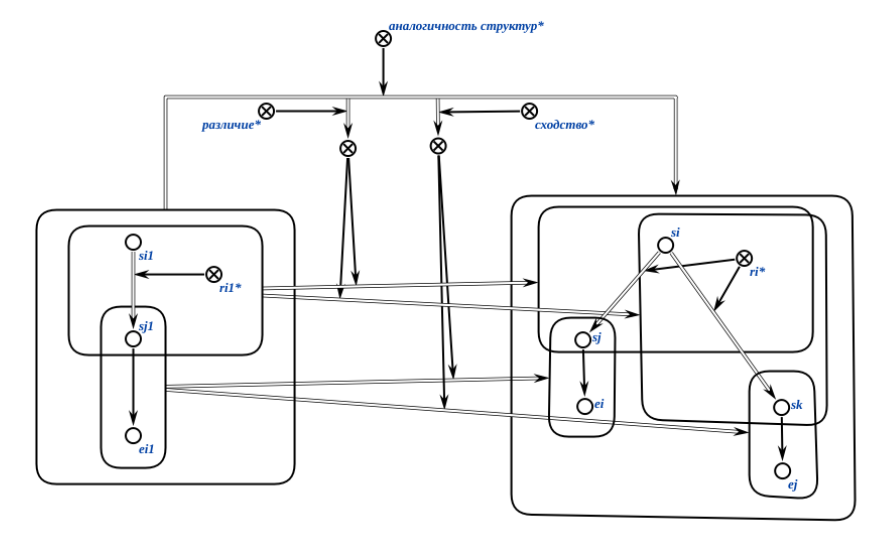
\includegraphics[scale=0.3]{./figures/sd_structures/analog.png}
	\end{figure}
\end{frame}

\begin{frame}{\\Понятие семантической окрестности}
	\topline
	\justifying
	
	\vspace{5mm}
	Для спецификации отдельных сущностей в рамках базы знаний вводится понятие семантической окрестности.\\
	Семантическая окрестность представляет собой спецификацию заданной сущности, знак которой указывается
	как ключевой элемент этой спецификации. В отличие от других видов знаний, семантическая окрестность имеет
	только один ключевой элемент.\\
	Набор признаков, по которым можно специфицировать сущности, различен. Кроме того, может возникнуть необходимость специфицировать одну и ту же сущность в различных аспектах и явно фиксировать эти аспекты в базе
	знаний.\\
	Так, например, одну и ту же персону можно описывать с профессиональной, медицинской, гражданской и других
	точек зрения
\end{frame}

\begin{frame}{\\Пример}
	\topline
	\justifying
	
	\begin{figure}[H]
		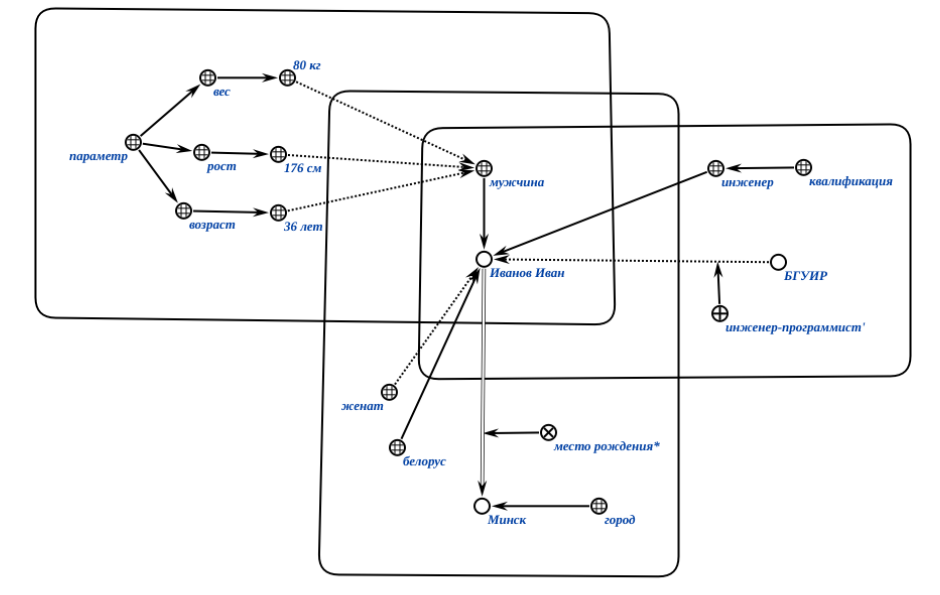
\includegraphics[scale=0.28]{./figures/sd_structures/example.png}
	\end{figure}
\end{frame}

\begin{frame}{\\Понятие семантической окрестности}
	\topline
	\justifying
	\scnheader{семантическая окрестность}
	\scnidtf{описание заданной сущности, знак которой указывается как ключевой элемент этой спецификации}
	\scnsubset{знание}
	\scnsuperset{семантическая окрестность по инцидентным коннекторам}
	\scnsuperset{полная семантическая окрестность}
	\scnsuperset{базовая семантическая окрестность}
	\scnsuperset{специализированная семантическая окрестность}
	
\end{frame}

\begin{frame}{\\Типология семантических окрестностей}
	\topline
	\justifying
	\scnheader{семантическая окрестность по инцидентным коннекторам}
	\scnsuperset{семантическая окрестность по выходящим дугам}
	\scnsuperset{семантическая окрестность по входящим дугам}
	\scnrelfrom{пояснение}{вид семантической окрестности, в которую входят все коннекторы, инцидентные заданному элементу, а также
	все элементы, инцидентные указанным коннекторам.}
\end{frame}

\begin{frame}{\\Типология семантических окрестностей}
	\topline
	\justifying
	\scnheader{полная семантическая окрестность}
	\scnidtf{полная спецификация некоторой описываемой сущности}
	
	\scnheader{базовая семантическая окрестность}
	\scnidtf{минимально достаточная семантическая окрестность}
	
	\scnheader{специализированная семантическая окрестность}
	\scnidtf{вид семантической окрестности, набор связей для которой уточняется отдельно для каждого типа такой окрестности.}
\end{frame}

\begin{frame}{\\Типология семантических окрестностей}
	\topline
	\justifying
	\scnheader{специализированная семантическая окрестность}
	\scnsuperset{пояснение}
	\scnsuperset{примечание}
	\scnsuperset{правило идентификации экземпляров}
	\scnsuperset{терминологическая семантическая окрестность}
	\scnsuperset{теоретико-множественная семантическая окрестность}
	\scnsuperset{логическая семантическая окрестность}
	\scnsuperset{описание типичного экземпляра}
	\scnsuperset{описание декомпозиции}
\end{frame}


\title{Лекция 9\\Представление логических знаний}
\author[]{Шункевич Д.В.}
\institute[]{Белорусский государственный университет информатики и радиоэлектроники}

\begin{frame}
	\titlepage
\end{frame}

\begin{comment}

\begin{frame}{\\Содержание лекции}
	\topline
	\justifying
	Формальные логические языки. Алфавит и синтаксис языка SCL. Предикаты и булевы функции. Логические связки (операторы), таблицы истинности. Логическая формула, равносильные логические формулы, логические законы. Классы логических формул. Кванторы, законы двойственности. Связанные и свободные переменные. Открытые и замкнутые формулы. Представление в базе знаний.
\end{frame}

\end{comment}

\begin{frame}{\\Формальный язык}
	\topline
	\justifying	
	\textbf{Формальный язык} -- множество конечных слов(строк) над конечным алфавитом
	Если \textit{L} -- формальный язык, а \textit{A} -- его алфафит, то $L \subseteq A^*$, где $A^*$ -- операция замыкания множества \textit{A}.\\
	Формальными логическими языками являются язык \textbf{логики высказываний} и язык \textbf{логики предикатов первого порядка}.	
\end{frame}

\begin{frame}{\\Формальный логический язык SCL}
	\topline
	\justifying
	Формальный логический язык SCL построен на базе языка SC как его подъязык путем фиксации определенного набора специальных ключевых узлов, т.е. узлов, семантика которых должна быть априори
	известна и согласована.\\
	Логический язык SCL является языком теоретико-множественного типа, в основе которого лежит трактовка логических связок и кванторов через понятия множества, кортежа, атрибута, отношения, т.е.
	трактовка формальных теорий и неатомарных логических формул как реляционных структур над высказываниями. 
\end{frame}

\begin{frame}{\\Формальный логический язык SCL}
	\topline
	\justifying
	Язык SCL является подъязыком языка SC и имеет две модификации:
	\begin{textitemize}
		\item{линейную модификацию – язык SCLs (Semantic Code Logic string);}
		\item{графическую модификацию – язык SCLg (Semantic Code Logic graphical). }
	\end{textitemize}
	Основное отличие языка SCLs от классического логического языка заключается в способе записи атомарных логических формул. Атомарная логическая формула в языке SCLs – это текст языка SCs, ограниченный квадратными скобками. Неатомарные (сложные) логические формулы в языке SCLs строятся точно так же, как и в классическом логическом языке.
\end{frame}

\begin{frame}{\\Предикат. Булева функция}
	\topline
	\justifying
	\textbf{Предикат} -- функция с областью значений $\{\top, \bot\}$ и областью определений $M^n$, где $M$ -- множество объектов предметной области.\\
	\textbf{Булева функция} -- функция с областью определения $B^n$ и областью значений $B$, где $B = \{\top, \bot\}$.\\
	\textbf{Булева функция} задаётся конечным набором значений, что позволяет представить её в виде таблицы истинности.
\end{frame}

\begin{frame}{\\Таблица истинности}
	\topline
	\justifying
	\textbf{Таблица истинности} -- таблица, устанавливающая соответствие между всеми возможными наборами логических переменных, входящих в логическую функцию, и значениями функции.\\
	\vspace{5mm}
	\begin{center}
		\begin{tabular}{|c|c|c|}
			\hline
			$X$ & $Y$ & $F(X,Y)$\\
			\hline
			$0$ & $0$ & $0$\\
			\hline
			$0$ & $1$ & $1$\\
			\hline
			$1$ & $0$ & $1$\\
			\hline
			$1$ & $1$ & $0$\\
			\hline
		\end{tabular}
	\end{center}
\end{frame}

\begin{frame}{\\Логические связки (операторы)}
	\topline
	\justifying
	\begin{SCn}
		\scnheader{логическая связка*}
		\scnidtf{неатомарная логическая формула}
		\scnidtf{логический оператор*}
		\scnidtf{пропозициональная связка*}
		\scniselement{класс связок разной мощности}
		\scnrelto{семейство подмножеств}{неатомарное высказывание}
		\scnrelfrom{пояснение}{
			\textbf{\textit{логическая связка*}} -- это отношение (класс связок), связками которого являются \textit{высказывания}.\\
			\textbf{\textit{логическая связка*}} -- это \textit{отношение}, областью определения которого является множество \textit{высказываний}, при этом само это отношение и некоторые его подмножества могут быть \textit{классами связок разной мощности}.
		}	
	\end{SCn}	
\end{frame}

\begin{frame}{\\Конъюнкция}
	\topline
	\justifying
	\small{
		\begin{SCn}
			\scnheader{конъюнкция*}
			\scnidtf{логическое и*}
			\scnidtf{логическое умножение*}
			\scnsubset{логическая связка*}
			\scniselement{неориентированное отношение}
			\scniselement{класс связок разной мощности}
			\scnrelfrom{пояснение}{
				\textbf{\textit{конъюнкция*}} -- это множество конъюнктивных \textit{высказываний}, каждое из которых истинно в рамках некоторой \textit{формальной теории} только в том случае, когда все его компоненты истинны в рамках этой же \textit{формальной теории}.
				\textbf{\textit{конъюнкция*}} атомарных формул может быть заменена на атомарную формулу, полученную путём объединения исходных атомарных формул.
			}
		\end{SCn}
	}	
\end{frame}

\begin{frame}{\\Конъюнкция}
	\topline
	\justifying
	\begin{figure}[H]
		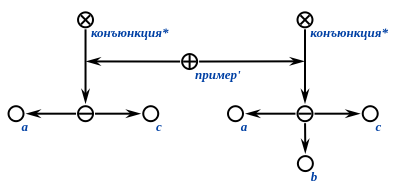
\includegraphics[scale=1.0]{./figures/sd_logic/conjunction.png}
	\end{figure}
\end{frame}

\begin{frame}{\\Дизъюнкция}
	\topline
	\justifying
	\small{
		\begin{SCn}
			\scnheader{дизъюнкция*}
			\scnidtf{логическое или*}
			\scnidtf{логическое сложение*}
			\scnidtf{включающее или*}
			\scnsubset{логическая связка*}
			\scniselement{неориентированное отношение}
			\scniselement{класс связок разной мощности}
			\scnrelfrom{пояснение}{
				\textbf{\textit{дизъюнкция*}} -- это множество дизъюнктивных \textit{высказываний}, каждое из которых истинно в рамках некоторой \textit{формальной теории} только в том случае, когда хотя бы один его компонент является истинным в рамках этой же \textit{формальной теории}.
			}
		\end{SCn}
	}
\end{frame}

\begin{frame}{\\Дизъюнкция}
	\topline
	\justifying
	\begin{figure}[H]
		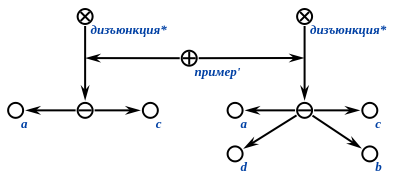
\includegraphics[scale=1.0]{./figures/sd_logic/disjunction.png}
	\end{figure}
\end{frame}

\begin{frame}{\\Отрицание}
	\topline
	\justifying
	\begin{SCn}
		\scnheader{отрицание*}
		\scnsubset{логическая связка*}
		\scnsubset{синглетон}
		\scnrelfrom{пояснение}{
			\textbf{\textit{отрицание*}} -- это множество \textit{высказываний} об отрицании, каждое из которых истинно в рамках некоторой \textit{формальной теории} только в том случае, когда его единственный элемент является ложным в рамках этой же \textit{формальной теории}.
		}
	\end{SCn}
\end{frame}

\begin{frame}{\\Отрицание}
	\topline
	\justifying
	\begin{figure}[H]
		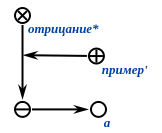
\includegraphics[scale=1.0]{./figures/sd_logic/negation.png}
	\end{figure}	
\end{frame}

\begin{frame}{\\Строгая дизъюнкция}
	\topline
	\justifying
	\begin{SCn}
		\scnheader{строгая дизъюнкция*}
		\scnidtf{сложение по модулю 2*}
		\scnidtf{исключающее или*}
		\scnidtf{альтернатива*}
		\scnsubset{логическая связка*}
		\scniselement{неориентированное отношение}
		\scniselement{класс связок разной мощности}
		\scnrelfrom{пояснение}{
			\textbf{\textit{строгая дизъюнкция*}} -- это множество строго дизъюнктивных \textit{высказываний}, каждое из которых истинно в рамках некоторой \textit{формальной теории} только в том случае, когда ровно один его компонент является истинным в рамках этой же \textit{формальной теории}.
		}
	\end{SCn}
\end{frame}

\begin{frame}{\\Строгая дизъюнкция}
	\topline
	\justifying
	\begin{figure}[H]
		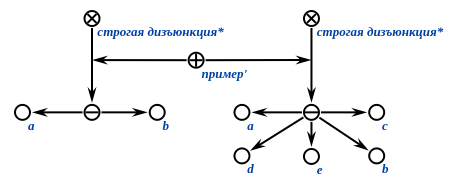
\includegraphics[scale=1.0]{./figures/sd_logic/strictDisjunction.png}
	\end{figure}	
\end{frame}

\begin{frame}{\\Импиликация}
	\topline
	\justifying
	\footnotesize{
		\begin{SCn}
			\scnheader{импликация*}
			\scnidtf{логическое следование*}
			\scnsubset{логическая связка*}
			\scniselement{бинарное отношение}
			\scniselement{ориентированное отношение}
			\scnrelfrom{пояснение}{
				\textbf{\textit{импликация*}} -- это множество импликативных \textit{неатомарных высказываний}, каждое из которых состоит из посылки (первый компонент \textit{высказывания}) и следствия (второй компонент \textit{высказывания}).
				Каждое импликативное \textit{высказывание} ложно в рамках некоторой \textit{формальной теории} в том случае, когда его посылка истинна, а заключение ложно в рамках этой же \textit{формальной теории}. В других случаях такое \textit{высказывание} истинно.
				По умолчанию на все переменные, входящие в обе части высказывания об \textbf{\textit{импликации*}} (или хотя бы одну из \textit{подформул*} каждой части) неявно накладывается квантор \textit{всеобщности*}, при условии, что эти переменные не связаны другим \textit{квантором}, указанным явно.
			}
		\end{SCn}
	}
\end{frame}

\begin{frame}{\\Импликация}
	\topline
	\justifying
	\begin{figure}[H]
		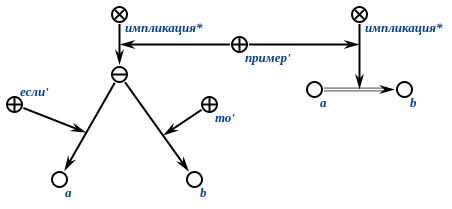
\includegraphics[scale=1.0]{./figures/sd_logic/implication.png}
	\end{figure}	
\end{frame}

\begin{frame}{\\Эквиваленция}
	\topline
	\justifying
	\footnotesize{
		\begin{SCn}
			\scnheader{эквиваленция*}
			\scnidtf{эквивалентность*}
			\scnsubset{логическая связка*}
			\scniselement{бинарное отношение}
			\scniselement{неориентированное отношение}
			\scnrelfrom{пояснение}{
				\textbf{\textit{эквиваленция*}} -- это множество \textit{высказываний} об эквивалентности, каждое из которых истинно в рамках некоторой \textit{формальной теории} только в тех случаях, когда оба его компонента одновременно либо истинны в рамках этой же \textit{формальной теории}, либо ложны.
				По умолчанию на все переменные, входящие в обе части высказывания об \textbf{\textit{эквиваленции*}} (или хотя бы одну из \textit{подформул*} каждой части) неявно накладывается квантор \textit{всеобщности*}, при условии, что эти переменные не связаны другим \textit{квантором}, указанным явно.
			}
		\end{SCn}
	}
\end{frame}

\begin{frame}{\\Эквиваленция}
	\topline
	\justifying
	\begin{figure}[H]
		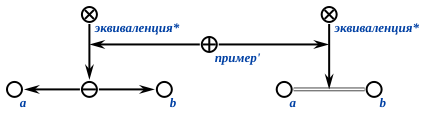
\includegraphics[scale=1.0]{./figures/sd_logic/equivalent.png}
	\end{figure}	
\end{frame}

\begin{frame}{\\ \small{Таблицы истинности логических функций}}
	\topline
	\justifying
	\vspace{5mm}
	\begin{center}
		\begin{tabular}{|c|c|c|c|c|c|c|c|}
			\hline
			$X$ & $Y$ & $\neg X$ & $X \land Y$ & $X \lor Y$ & $X \oplus Y$ & $X \to Y$ & $X \leftrightarrow Y$\\
			\hline
			$0$ & $0$ & $1$ & $0$ & $0$ & $0$ & $1$ & $1$\\
			\hline
			$0$ & $1$ & $1$ & $0$ & $1$ & $1$ & $1$ & $0$\\
			\hline
			$1$ & $0$ & $0$ & $0$ & $1$ & $1$ & $0$ & $0$\\
			\hline
			$1$ & $1$ & $0$ & $1$ & $1$ & $0$ & $1$ & $1$\\
			\hline
		\end{tabular}
	\end{center}
\end{frame}

\begin{frame}{\\Высказывание}
	\topline
	\justifying
	\begin{SCn}
			\scnheader{высказывание}
		\scnrelfrom{пояснение}{
			Под \textbf{\textit{высказыванием}} понимается некоторая \textit{структура} (в которую входят \textit{sc-константы} из некоторой предметной области и/или \textit{sc-переменные}) или \textit{логическая связка}, которая может трактоваться как истинная или ложная в рамках какой-либо \textit{предметной области}.			
		}
		\begin{scnreltoset}{\textit{разбиение}}
			\scnitem{атомарное высказывание}
			\scnitem{неатомарное высказывание}
		\end{scnreltoset}
		\begin{scnreltoset}{\textit{разбиение}}
			\scnitem{фактографическое высказывание}
			\scnitem{логическая формула}
		\end{scnreltoset}
	\end{SCn}
\end{frame}

\begin{frame}{\\Высказывание}
	\topline
	\justifying
	\\	
	Истинность \textbf{\textit{высказывания}} задается путем указания принадлежности знака этого высказывания \textit{формальной теории}, соответствующей данной \textit{предметной области}. Ложность высказывания задается путем указания принадлежности знака \textit{отрицания*} этого высказывания данной \textit{формальной теории}.\\
	Явно указанная непринадлежность \textbf{\textit{высказывания}} \textit{формальной теории} может говорить как о его ложности в рамках данной теории (если это указано рассмотренным выше образом), так и о том, что данное  \textbf{\textit{высказывание}} вообще не рассматривается в данной \textit{формальной теории} (например, использует понятия, не принадлежащие данной \textit{предметной области}).\\
	Одно и то же \textbf{\textit{высказывание}} может быть истинно в рамках одной \textit{формальной теории} и ложно в рамках другой.
\end{frame}

\begin{frame}{\\Высказывание формальной теории}
	\topline
	\justifying
	\begin{SCn}
		\scnheader{высказывание формальной теории\scnrolesign}
		\scniselement{неосновное понятие}
		\begin{scnreltoset}{разбиение}
			\scnitem{истинное высказывание\scnrolesign}			
			\scnitem{ложное высказывание\scnrolesign}			
			\scnitem{нечеткое высказывание\scnrolesign}			
			\scnitem{бессмысленное высказывание\scnrolesign}			
		\end{scnreltoset}
	\end{SCn}	
\end{frame}

\begin{frame}{\\ \small{Истинное высказывание. Ложное высказывание.}}
	\topline
	\justifying	
	\begin{SCn}
		\scnheader{истинное высказывание\scnrolesign}
		\scnidtf{высказывание, истинное в рамках данной формальной теории\scnrolesign}
		\scnidtf{высказывание, знак которого принадлежит данной формальной теории\scnrolesign}
		\scnheader{ложное высказывание\scnrolesign}
		\scnidtf{высказывание, ложное в рамках данной формальной теории\scnrolesign}
		\scnidtf{высказывание, знак отрицания которого принадлежит данной формальной теории\scnrolesign}		
	\end{SCn}	
\end{frame}

\begin{frame}{\\ \small{Нечёткое высказывание. Бессмысленное высказывание}}
	\topline
	\justifying
	\begin{SCn}
		\small{
			\scnheader{нечеткое высказывание\scnrolesign}
			\scnidtf{гипотетическое высказывание\scnrolesign}
			\scnidtf{высказывание, возможно истинное или ложное в рамках данной формальной теории\scnrolesign}
			\scnidtf{высказывание, истинное или ложное в рамках данной формальной теории с некоторой вероятностью\scnrolesign}
			\scnheader{бессмысленное высказывание\scnrolesign}
			\scnidtf{высказывание, бессмысленное в рамках данной формальной теории\scnrolesign}
			\scnidtf{высказывание, не рассматриваемое в рамках данной формальной теории\scnrolesign}
			\scnrelfrom{пояснение}{
				Высказывание является бессмысленным в рамках заданной формальной теории, если в какое-либо \textit{атомарное высказывание} в его составе (или в само это высказывание, если оно является атомарным) входит какая-либо \textit{sc-константа}, не являющаяся элементом предметной области, описываемой указанной \textit{формальной теорией}.			
			}
		}
	\end{SCn}
\end{frame}

\begin{frame}{\\ \small{Атомарное высказывание. Неатомарное высказывание}}
	\topline
	\justifying
	\footnotesize{
		\begin{SCn}
			\scnheader{атомарное высказывание}
			\scnsubset{структура}
			\begin{scnreltoset}{разбиение}
				\scnitem{атомарное фактографическое высказывание}			
				\scnitem{атомарная логическая формула}						
			\end{scnreltoset}
			\scnrelfrom{пояснение}{
				\textbf{\textit{атомарное высказывание}} -- это \textit{высказывание}, которое содержит хотя бы один \textit{sc-элемент}, не являющийся знаком другого \textit{высказывания}.
			}
			\scnheader{неатомарное высказывание}
			\scnrelfrom{пояснение}{
				\textbf{\textit{неатомарное высказывание}} -- это \textit{высказывание}, в состав которого входят только знаки других \textit{высказываний}.
				Следует отметить, что мы не можем говорить об истинности либо ложности \textbf{\textit{неатомарного высказывания}} в рамках какой-либо \textit{формальной теории}, в случае, когда невозможно установить истинность либо ложность любого из его элементов в рамках этой же \textit{формальной теории}.
			}			
		\end{SCn}
	}
\end{frame}

\begin{frame}{\\Фактографическое высказывание}
	\topline
	\justifying
	\begin{SCn}
		\scnheader{фактографическое высказывание}
		\scnsuperset{атомарное фактографическое высказывание}
		Под \textbf{фактографическим высказыванием} понимается:
		\begin{textitemize}
			\item{\textit{атомарное высказывание}, в состав которого не входит ни одна \textit{sc-переменная}}
			\item{\textit{неатомарное высказывание}, все элементы которого также являются \textbf{\textit{фактографическими высказываниями}}}
		\end{textitemize}
	\end{SCn}
\end{frame}

\begin{frame}{\\Логическая формула}
	\topline
	\justifying	
	\begin{SCn}
		\footnotesize{
			Под \textbf{логической формулой} понимается:
			\begin{textitemize}
				\item{\textit{атомарное высказывание}, в состав которого входит хотя бы одна \textit{sc-переменная};}
				\item{\textit{неатомарное высказывание}, хотя бы один элемент которого является \textbf{\textit{логической формулой}}.}
			\end{textitemize}		
			\scnheader{логическая формула}
			\begin{scnreltoset}{разбиение}
				\scnitem{атомарная логическая формула}			
				\scnitem{неатомарная логическая формула}						
			\end{scnreltoset}
			\begin{scnreltoset}{разбиение}
				\scnitem{открытая логическая формула}			
				\scnitem{замкнутая логическая формула}						
			\end{scnreltoset}
		}
	\end{SCn}
\end{frame}

\begin{frame}{\\Равносильность логических формул}
	\topline
	\justifying
	\\
	\footnotesize{
		Две формулы логики $A$ и $B$ называются равносильными, если они принимают одинаковые логические значения при любом наборе значений входящих в формулы элементарных высказываний (переменных).\\
		\textit{Обозначение}: $A \iff B$
		\begin{center}
			\begin{tabular}{|c|c|}
				\hline
				$X \land X \iff X$ & $X \lor X \iff X$\\
				\hline
				$X \land \top X \iff X$ & $X \lor \top \iff \top$\\
				\hline
				$X \land \bot \iff \bot$ & $X \lor \bot \iff X$\\
				\hline
				$X \land \neg X \iff \bot$ & $X \lor \neg X \iff \top$\\
				\hline
				$\neg(\neg X) \iff X$ & $X \lor (Y \land X) \iff X$\\
				\hline
				$X \land (Y \lor X) \iff X$ & $X \leftrightarrow Y \iff (X \leftarrow Y) \land (Y \leftarrow X)$\\
				\hline
				$X \leftarrow Y \iff \neg X \lor Y$ & $\neg(X \land Y) \iff \neg X \lor \neg Y$\\
				\hline
				$\neg(X \lor Y) \iff \neg X \land \neg Y$ & $X \land Y \iff \neg(\neg X \lor \neg Y)$\\
				\hline
				$X \lor Y \iff \neg(\neg X \land \neg Y)$ &\\
				\hline
			\end{tabular}
		\end{center}
	}
\end{frame}

\begin{frame}{\\Тавтология}
	\topline
	\justifying
	\begin{SCn}
		\scnheader{тавтология}
		\scnrelfrom{пояснение}{
			\textbf{\textit{тавтология}} -- это \textit{логическая формула}, которая является либо только истинной, либо только ложной в рамках всех \textit{формальных теорий}, в которых можно установить ее истинность или ложность.\\
			\textbf{\textit{тавтология}} -- это такая \textit{логическая формула}, которая является либо \textit{общезначимой логической формулой}, либо \textit{противоречивой логической формулой}.
		}
	\end{SCn}
\end{frame}

\begin{frame}{\\Общезначимая логическая формула}
	\topline
	\justifying
	\begin{SCn}
		\scnheader{общезначимая логическая формула}
		\scnidtf{тождественно истинная логическая формула}
		\scnsubset{выполнимая логическая формула}
		\scnsubset{тавтология}
		\scnrelfrom{пояснение}{
			\textbf{\textit{общезначимая логическая формула}} -- это \textit{логическая формула}, для которой не существует \textit{формальной теории}, в рамках которой она была бы ложной с учетом истинности и ложности всех ее \textit{подформул*} в рамках этой же \textit{формальной теории}.
		}
	\end{SCn}
\end{frame}

\begin{frame}{\\Общезначимая логическая формула}
	\topline
	\justifying
	\begin{figure}[H]
		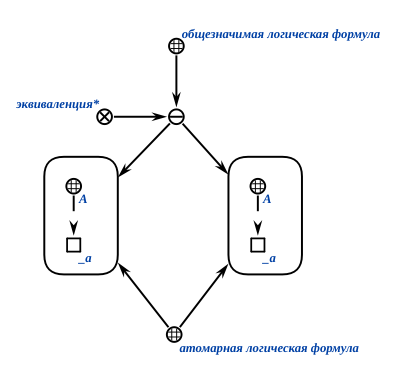
\includegraphics[scale=0.7]{./figures/sd_logic/valid_formula.png}
	\end{figure}	
\end{frame}

\begin{frame}{\\Противоречивая логическая формула}
	\topline
	\justifying
	\begin{SCn}
		\scnheader{противоречивая логическая формула}
		\scnidtf{тождественно ложная логическая формула}
		\scnsubset{невыполнимая логическая формула}
		\scnsubset{тавтология}
		\scnrelfrom{пояснение}{
			\textbf{\textit{противоречивая логическая формула}} -- это \textit{логическая формула}, для которой не существует \textit{формальной теории}, в рамках которой она была бы истинной с учетом истинности и ложности всех ее \textit{подформул*} в рамках этой же \textit{формальной теории}.
		}
	\end{SCn}
\end{frame}

\begin{frame}{\\Противоречивая логическая формула}
	\topline
	\justifying
	\begin{figure}[H]
		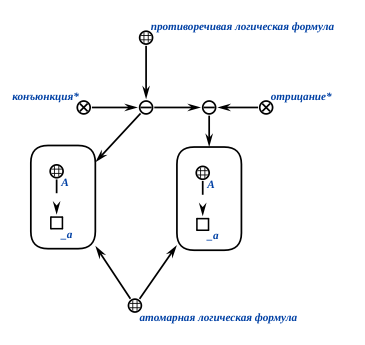
\includegraphics[scale=0.7]{./figures/sd_logic/contradiction_formula.png}
	\end{figure}	
\end{frame}

\begin{frame}{\\Нейтральная логическая формула}
	\topline
	\justifying
	\begin{SCn}
		\scnheader{нейтральная логическая формула}
		\scnsubset{выполнимая логическая формула}
		\scnrelfrom{пояснение}{
			\textbf{\textit{нейтральная логическая формула}} -- это \textit{логическая формула}, для которой существует хотя бы одна \textit{формальная теория}, в рамках которой эта формула ложна, и хотя бы одна \textit{формальная теория}, в рамках которой эта формула истинна.
		}
	\end{SCn}
\end{frame}

\begin{frame}{\\Нейтральная логическая формула}
	\topline
	\justifying
	\begin{figure}[H]
		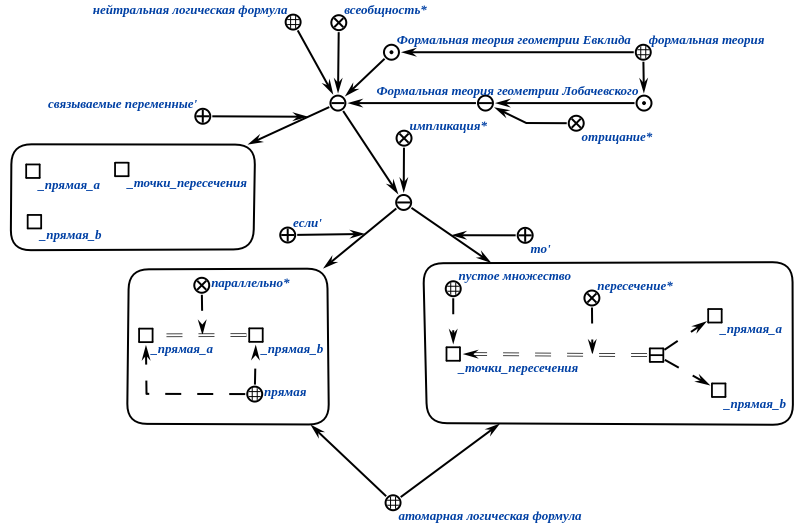
\includegraphics[scale=0.45]{./figures/sd_logic/neutral_formula.png}
	\end{figure}	
\end{frame}

\begin{frame}{\\Непротиворечивая логическая формула}
	\topline
	\justifying
	\begin{SCn}
		\scnheader{Непротиворечивая логическая формула}
		\scnidtf{выполнимая логическая формула}
		\scnrelfrom{пояснение}{
			\textbf{\textit{непротиворечивая логическая формула}} -- это \textit{логическая формула}, для которой существует хотя бы одна \textit{формальная теория}, в рамках которой эта формула истинна.
		}
		\begin{scnreltoset}{объединение}
			\scnitem{нейтральная логическая формула}
			\scnitem{общезначимая логическая формула}
		\end{scnreltoset}	
	\end{SCn}
\end{frame}

\begin{frame}{\\Необщезначная логическая формула}
	\topline
	\justifying
	\begin{SCn}
		\scnheader{необщезначимая логическая формула}
		\scnidtf{невыполнимая логическая формула}
		\scnrelfrom{пояснение}{
			\textbf{\textit{необщезначимая логическая формула}} -- это \textit{логическая формула}, для которой существует хотя бы одна \textit{формальная теория}, в рамках которой эта формула ложна.
		}
		\begin{scnreltoset}{объединение}
			\scnitem{нейтральная логическая формула}
			\scnitem{противоречивая логическая формула}
		\end{scnreltoset}
	\end{SCn}
\end{frame}

\begin{frame}{\\Квантор}
	\topline
	\justifying
	\begin{SCn}
		\scnheader{квантор}
		\scnsubset{логическая связка*}
		\scnrelfrom{пояснение}{
			\textbf{\textit{квантор}} — это \textit{отношение}, каждая связка которой задает истинность множества \textit{логических формул}, входящих в ее состав, при выполнении дополнительных условий, связанных с некоторыми из переменных, входящих в состав этих \textit{логических формул}.\\
			Будем говорить, что переменные связаны \textbf{\textit{квантором}} или попадают под область действия данного \textbf{\textit{квантора}} (имея в виду конкретную связку конкретного \textbf{\textit{квантора}}).\\
			В состав каждой связки каждого \textbf{\textit{квантора}} входит \textit{атомарная формула}, являющаяся \textit{тривиальной структурой}, в которой перечислены переменные, связанные данным \textbf{\textit{квантором}}.
		}
	\end{SCn}
\end{frame}

\begin{frame}{\\Квантор всеобщности}
	\topline
	\justifying
	\footnotesize{
		\begin{SCn}
			\scnheader{всеобщность*}
			\scnidtf{квантор всеобщности*}
			\scnidtf{квантор общности*}
			\scniselement{квантор}
			\scniselement{ориентированное отношение}
			\scniselement{класс связок разной мощности}
			\scnrelfrom{пояснение}{
				\textbf{\textit{всеобщность}} -- это \textit{квантор}, для каждой связки которого, истинной в рамках некоторой \textit{формальной теории}, выполняется следующее утверждение: все формулы, входящие в состав этой связки истинны в рамках этой же \textit{формальной теории} при всех (любых) возможных значениях всех элементов множества \textit{связываемых переменных\scnrolesign} входящего в эту связку.\\
				Каждая связка \textit{квантора} \textbf{\textit{всеобщность*}} может быть представлена как \textit{конъюнкция*} (потенциально бесконечная) исходных \textit{логических формул}, входящих в состав этой связки, в каждой из которых все \textit{связанные переменные\scnrolesign} заменены на их возможные значения.
				Квантор \textbf{\textit{всеобщности*}} зачастую обозначается "$\forall$" \ и читается как "для всех"{}, "для каждого"{}, "для любого"{} или "все"{}, "каждый"{}, "любой".
			}
		\end{SCn}
	}
\end{frame}

\begin{frame}{\\Квантор всеобщности}
	\topline
	\justifying
	\begin{figure}[H]
		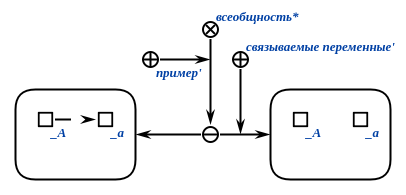
\includegraphics[scale=1.0]{./figures/sd_logic/universality.png}
	\end{figure}	
\end{frame}

\begin{frame}{\\Квантор существования}
	\topline
	\justifying
	\begin{SCn}
		\scnheader{формула существования}
		\scnidtf{существование*}
		\begin{scnreltoset}{разбиение}
			\scnitem{атомарная логическая формула}
			\scnitem{неатомарное существование*}
		\end{scnreltoset}
	\end{SCn}
\end{frame}

\begin{frame}{\\Неатомарное существование}
	\topline
	\justifying
	\footnotesize{
		\begin{SCn}
			\scnheader{неатомарное существование*}
			\scnidtf{квантор неатомарного существования*}
			\scniselement{квантор}
			\scniselement{ориентированное отношение}
			\scniselement{класс связок разной мощности}
			\scnrelfrom{пояснение}{
				\textbf{\textit{неатомарное существование*}} -- это \textit{квантор}, для каждой связки которого, истинной в рамках некоторой \textit{формальной теории}, выполняется следующее утверждение: существуют значения всех элементов множества \textit{связываемых переменных\scnrolesign} входящего в эту связку, такие, что все формулы, входящие в состав этой связки истинны в рамках этой же \textit{формальной теории}.\\
				Каждая связка \textit{квантора} \textbf{\textit{неатомарное существование*}} может быть представлена как \textit{дизъюнкция*} (потенциально бесконечная) исходных \textit{логических формул}, входящих в состав этой связки, в каждой из которых все \textit{связанные переменные\scnrolesign} заменены на их возможные значения.
				Квантор \textbf{\textit{существования*}} зачастую обозначается "$\exists$" \ и читается как "существует"{}, "для некоторого"{}, "найдется".
			}
		\end{SCn}
	}
\end{frame}

\begin{frame}{\\Неатомарное существование}
	\topline
	\justifying
	\begin{figure}[H]
		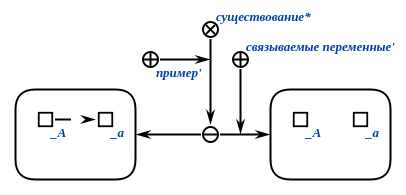
\includegraphics[scale=1.0]{./figures/sd_logic/non_atomicExistence.png}
	\end{figure}	
\end{frame}

\begin{frame}{\\Единственное существование}
	\topline
	\justifying
	\begin{SCn}
		\scnheader{единственное существование}
		\scnidtf{однократное существование}
		\scnidtf{формула существования и единственности}
		\scnrelfrom{пояснение}{
			\textbf{\textit{единственное существование}} зачастую обозначается "$\exists!$" \ и читается как "существует и единственный".
		}
	\end{SCn}
\end{frame}

\begin{frame}{\\Единственное существование}
	\topline
	\justifying
	\begin{SCn}
		\scnheader{логическая формула и единственность}
		\scnsubset{логическая формула}
		\scnsubset{единственное существование}
		\scnrelfrom{пояснение}{
			Каждый элемент множества \textbf{\textit{логическая формула и единственность}} представляет собой \textit{логическую формулу} (\textit{атомарную} или \textit{неатомарную}), для которой дополнительно уточняется, что при ее интерпретации на некоторой предметной области существует только один набор значений переменных, входящих в эту формулу (или ее \textit{подформулы*}), при котором указанная логическая формула истинна в рамках \textit{формальной теории}, в которую входит данная \textit{предметная область}.
		}
	\end{SCn}
\end{frame}

\begin{frame}{\\Единственное существование}
	\topline
	\justifying
	\begin{figure}[H]
		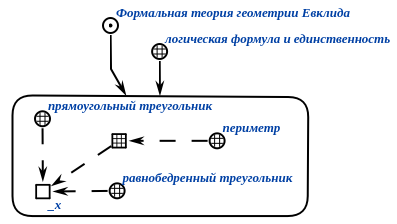
\includegraphics[scale=1.0]{./figures/sd_logic/unique_existance.png}
	\end{figure}	
\end{frame}

\begin{frame}{\\Двойственность кванторов}
	\topline
	\justifying
	\textbf{Двойственность} -- содержательное понятие, применяемое в логике и математике всякий раз, когда между двумя группами понятий установлено взаимно-однозначное соответствие так, что замена понятий одной группы на соответствующие понятия др. группы каждый раз переводит истинные высказывания в истинные высказывания.\\
	Двойственность кванторов:
	\begin{center}
		$\neg(\forall xA(x)) \iff \exists x(\neg A(x))$\\
		$\neg(\exists xA(x)) \iff \forall x(\neg A(x))$
	\end{center}
\end{frame}

\begin{frame}{\\Связываемые переменные}
	\topline
	\justifying
	\footnotesize{
		\begin{SCn}
			\scnheader{связываемые переменные\scnrolesign}
			\scniselement{ролевое отношение}
			\scnrelfrom{пояснение}{
				\textbf{\textit{связываемые переменные\scnrolesign}} -- это \textit{ролевое отношение}, которое связывает связку конкретного \textit{квантора} с множеством переменных, которые связаны этим квантором.
			}
			\scnheader{открытая логическая формула}
			\scnrelfrom{пояснение}{
				\textbf{\textit{открытая логическая формула}} -- это \textit{логическая формула}, в рамках которой (и всех ее \textit{подформул*}) существует хотя бы одна переменная, не связанная никаким \textit{квантором}.
			}
			\scnheader{замкнутая логическая формула}
			\scnrelfrom{пояснение}{
				\textbf{\textit{замкнутая логическая формула}} -- это \textit{логическая формула}, в рамках которой (и всех ее \textit{подформул*}) не существует переменных, не связанных каким-либо \textit{квантором}.
			}
		\end{SCn}
	}
\end{frame}


\title{Лекция 10\\Представление в базе знаний соответствий}
\author[]{Шункевич Д.В.}
\institute[]{Белорусский государственный университет информатики и радиоэлектроники}

\begin{frame}
	\titlepage
\end{frame}

\begin{frame}{\\Содержание лекции}
	\topline
	\justifying
	Типология соответствий. Однозначные и неоднозначные соответствия. Область определения и область значений соответствия, образ и прообраз. Отображения и биективные соответствия. Соответствия на структурах. Гомоморфизмы, изоморфизмы, автоморфизмы, представление в базе знаний.
\end{frame}

\begin{frame}{\\Типология соответствий}
\topline
\begin{SCn}
\scnheader{соответствие*}
\scnidtf{наличие соответствия*}
\begin{scnrelfromset}{разбиение}
        \scnitem{однозначное соответствие*}
	\scnitem{неоднозначное соответствие*}
\end{scnrelfromset}
\begin{scnrelfromset}{разбиение}
        \scnitem{всюду определенное соответствие*}
	\scnitem{частично определенное соответствие*}
\end{scnrelfromset}
\begin{scnrelfromset}{разбиение}
        \scnitem{сюръекция*}
	\scnitem{несюръективное соответствие*}
\end{scnrelfromset}
\end{SCn}
\end{frame}

\begin{frame}{\\Однозначное соответствие}
\topline
\begin{SCn}
\scnheader{однозначное соответствие*}
\scnidtf{наличие однозначного соответствия*}
\scnidtf{функциональное соответветствие*}
\scnidtf{функция*}
    \scnrelfrom{определение}{\normalfont{[}однозначное соответствие* – это соответствие*, при котором каждому элементу из области отправления’ соответствия ставится не более, чем один элемент из области прибытия’ соответствия.\normalfont{]}}
\end{SCn}
\end{frame}

\begin{frame}{\\Однозначное соответствие}
    \topline
    \begin{center}
        \begin{figure}[Hb]
            \centering
            \includegraphics[scale=.72]{figures/sd_correspondences/One-to-one correspondence.png}
        \end{figure}
    \end{center}
\end{frame}

\begin{frame}{\\Неоднозначное соответствие}
\topline
\begin{SCn}
\scnheader{неоднозначное соответствие*}
\scnrelfrom{определение}{\normalfont{[}неоднозначное соответствие* – это соответствие*, при котором хотя бы одному элементу из области отправления соответствия ставится более, чем один элемент из области прибытия соответствия.\normalfont{]}}
\end{SCn}
\end{frame}

\begin{frame}{\\Неоднозначное соответствие}
    \topline
    \begin{center}
        \begin{figure}[Hb]
            \centering
            \includegraphics[scale=.72]{figures/sd_correspondences/Ambiguous correspondence.png}
        \end{figure}
    \end{center}
\end{frame}

\begin{frame}{\\Область определения соответствия}
\topline
\begin{SCn}
\scnheader{область определения соответствия\scnrolesign}
\scnidtf{область отправления соответствия\scnrolesign}
\scnidtf{первый компонент пары в отношении соответствия\scnrolesign}
\scniselement{ролевое отношение}
\scnrelfrom{определение}{\normalfont{[}область определения соответствия\scnrolesign – ролевое отношение, указывающее на первый компонент пары в рамках отношения соответствие*.\normalfont{]}}
\end{SCn}
\end{frame}

\begin{frame}{\\Область значений соответствия}
\topline
\begin{SCn}
\scnheader{область значений соответствия\scnrolesign}
\scnidtf{область прибытия соответствия\scnrolesign}
\scnidtf{второй компонент пары в отношении соответствия\scnrolesign}
\scniselement{ролевое отношение}
\scnrelfrom{определение}{\normalfont{[}область прибытия – ролевое отношение, указывающее на второй компонент пары в рамках отношения соответствие*\normalfont{]}}
\end{SCn}
\end{frame}

\begin{frame}{\\Образ соответствия}
\topline
\begin{SCn}
\scnheader{образ\scnrolesign}
\scnidtf{образ соответствия\scnrolesign}
\scniselement{ролевое отношение}
\scnidtf{второй компонент пары в отношении соответствия\scnrolesign}
\scnrelfrom{определение}{\normalfont{[}образ\scnrolesign – ролевое отношение, указывающее на второй компонент каждой пары в рамках множества пар, которое является вторым компонентом отношения соответствия*.\normalfont{]}}
\end{SCn}
\end{frame}

\begin{frame}{\\Прообраз соответствия}
\topline
\begin{SCn}
\scnheader{прообраз\scnrolesign}
\scnidtf{прообраз соответствия\scnrolesign}
\scniselement{ролевое отношение}
\scnidtf{первый компонент пары в отношении соответствия\scnrolesign}
\scnrelfrom{определение}{\normalfont{[}прообраз\scnrolesign – ролевое отношение, указывающее на первый компонент каждой пары в рамках множества пар, которое является первым компонентом отношения соответствия*.\normalfont{]}
}
\end{SCn}
\end{frame}

\begin{frame}{\\Отображение}
\topline
\begin{SCn}
\scnheader{отображение*}
\scnsubset{всюду определённое соответствие*}
\scnsubset{однозначное соответствие*}
\scnrelfrom{определение}{\normalfont{[}отображение* – однозначное, всюду определённое соответствие.\normalfont{]}
}
\end{SCn}
\end{frame}

\begin{frame}{\\Отображение}
    \topline
    \begin{center}
        \begin{figure}[Hb]
            \centering
            \includegraphics[scale=.45]{figures/sd_correspondences/Display.jpeg}
        \end{figure}
    \end{center}
\end{frame}

\begin{frame}{\\Биективное соответствие}
\topline
\begin{SCn}
\scnheader{биективное соответствие*}
\scnidtf{биекция*}
\scnidtf{взаимно однозначное соответствие*}
\scnsubset{всюду определённое соответствие*}
\scnsubset{однозначное соответствие*}
\scnsubset{сюръективное соответствие*}
\scnrelfrom{определение}{\normalfont{[}биективное соответствие* – однозначное, всюду определённое, сюръективное соответствие.\normalfont{]}
}
\end{SCn}
\end{frame}

\begin{frame}{\\Биективное соответствие}
    \topline
    \begin{center}
        \begin{figure}[Hb]
            \centering
            \includegraphics[scale=.45]{figures/sd_correspondences/Bijection.jpeg}
        \end{figure}
    \end{center}
\end{frame}

\begin{frame}{\\Соответствия на структурах}
\topline
\begin{SCn}
Структура – множество sc-элементов, удаление одного из которых может привести к нарушению целостности этого множества.

Между структурами можно определять ряд соответствий, таких как \textbf{гомоморфизм, автоморфизм, изоморфизм}, а также аналогичность структур, что позволяет фиксировать факт наличия некоторой аналогии,
сходства и различия некоторых подструктур рассматриваемых структур.
\end{SCn}
\end{frame}

\begin{frame}{\\Гомоморфизм}
\topline
\begin{SCn}
\scnheader{гомоморфность*}
\scnidtf{гомоморфность структур*}
\scnsubset{соответствие*}
\scniselement{бинарное отношение}
\scnrelfrom{пояснение}{\normalfont{[}гомоморфность* - это соответствие, заданное на структурах, при котором каждому элементу из области определения соответствия (первой структуры) ставится в соответствие только один элемент из области значения соответствия (второй структуры).\normalfont{]}}

\scnheader{гомоморфизм*}
\scniselement{бинарное отношение}
\end{SCn}
\end{frame}

\begin{frame}{\\Гомоморфизм}
    \topline
    \begin{center}
        \begin{figure}[b]
            \centering
            \includegraphics[scale=.45]{figures/sd_correspondences/Homomorphism.png}
        \end{figure}
    \end{center}
\end{frame}

\begin{frame}{\\Изоморфизм}
\topline
\begin{SCn}
\scnheader{изоморфность*}
\scnidtf{изоморфность структур*}
\scnsubset{соответствие*}
\scniselement{бинарное отношение}
\scnrelfrom{пояснение}{\normalfont{[}изоморфность* - это гомоморфность*, при которой для каждого элемента из области значения существует ровно один соответствующий элемент из области определения.\normalfont{]}}

\scnheader{изоморфизм*}
\scniselement{бинарное отношение}
\end{SCn}
\end{frame}

\begin{frame}{\\Изоморфизм}
    \topline
    \begin{center}
        \begin{figure}[b]
            \centering
            \includegraphics[scale=.5]{figures/sd_correspondences/Isomorphism.png}
        \end{figure}
    \end{center}
\end{frame}

\begin{frame}{\\Автоморфизм}
\topline
\begin{SCn}
\scnheader{автоморфность*}
\scnidtf{автоморфность структур*}
\scnsubset{соответствие*}
\scniselement{бинарное отношение}
\scnrelfrom{пояснение}{\normalfont{[}автоморфность* - это изоморфность*, у которой область определения соответствия и область значения соответствия совпадают.\normalfont{]}}

\scnheader{автоморфизм*}
\scniselement{бинарное отношение}
\end{SCn}
\end{frame}

\begin{frame}{\\Автоморфизм}
    \topline
    \begin{center}
        \begin{figure}[b]
            \centering
            \includegraphics[scale=.55]{figures/sd_correspondences/Automorphism.png}
        \end{figure}
    \end{center}
\end{frame}
\title{Лекция 11\\Базовый язык программирования для обработки баз знаний}
\author[]{Шункевич Д.В.}
\institute[]{Белорусский государственный университет информатики и радиоэлектроники}

\begin{frame}
	\titlepage
\end{frame}

\begin{frame}{\\Содержание лекции}
	\topline
	\justifying
	Базовые принципы обработки знаний. 1-2-3-элементные конструкции. Произвольные конструкции, поиск и генерация по образцу. Основные положения языка SCP. Понятие scp-программы, scp-процесса, scp-оператора. Понятие scp-операнда, классификация scp-операндов, scp-переменная, scp-константа. Классификация scp-операторов. Организация условных и безусловных переходов, циклов. Реализация подпрограмм. Агентная scp-программа.
\end{frame}

%KB development
\title{Лекция 12\\Представление в базе знаний предметных областей}
\author[]{Шункевич Д.В.}
\institute[]{Белорусский государственный университет информатики и радиоэлектроники}

\begin{frame}
	\titlepage
\end{frame}

\begin{frame}{\\Содержание лекции}
	\topline
	\justifying
	Понятие знания, типология знаний. Понятие предметной области, структурная спецификация предметной области, роли понятий в рамках предметной области. Понятие частной предметной области, родственной предметной области, виды частных предметных областей. Различные виды иерархии предметных областей, пересечения предметных областей.
\end{frame}

\begin{frame}{\\Понятие знания}
	\begin{SCn}
		\scnheader{знание}
		\begin{scnrelfromset}{свойства}
			\scnitem{синтаксическая целостность}
				\begin{scnindent}
					\scnrelfrom{пояснение}{корректность}
				\end{scnindent}
			\scnitem{семантическая целостность}
			\begin{scnindent}
				\scnrelfrom{пояснение}{смысл}
			\end{scnindent}
		\end{scnrelfromset}
	\end{SCn}
\end{frame}

\begin{frame}{Классификация знаний}
	\begin{SCn}
		\scnheader{вид знаний}
		\scnidtf{класс знаний}
		\scnhaselement{задача}
		\scnhaselement{спецификация}
			\begin{scnindent}
				\scnidtf{семантическая окрестность}
			\end{scnindent}
			\begin{scnindent}
					\scnsuperset{параметрическая модель}
					\scnsuperset{семантическая окрестность}
						\begin{scnindent}
							\scnidtf{набор свойств, которые описывают сущность}
						\end{scnindent}
					\scnsuperset{сходство}
					\scnsuperset{отличие}
					\scnsuperset{достоинства}
					\scnsuperset{недостатки}
					\scnsuperset{сравнение}
			\end{scnindent}
	\end{SCn}
\end{frame}

\begin{frame}{\\***}
	\begin{SCn}
			\scnheader{вид знаний}
				\scnhaselement{высказывание}
			\scnhaselement{формальная теория}
			\scnhaselement{предметная область и онтология}
			\scnhaselement{метазнание}
			\begin{scnindent}
				\scnsuperset{введение}
				\scnsuperset{заключение}
				\scnsuperset{выводы}
				\scnsuperset{онтология}
			\end{scnindent}
	\end{SCn}
\end{frame}

\begin{frame}{\\Понятие предметной области}
	\begin{SCn}
		\scnheader{предметная область}
		\scnidtf{объединение частичных семантических окрестностей, описывающих все сущности класса и имеющих одинаковых предмет исследования (набор отношений)}
		\scnidtf{структура из экзмепляров классов, связей}
		\scnheader{онтология}
		\scnidtf{вид знаний}
		\scnidtf{спецификация (описание свойств) предметной области}        
		\scnheader{интегрированная онтология}
		\scnidtf{объединение всех видов онтологии заданной предметной области}
	\end{SCn}
\end{frame}

\begin{frame}{Частная предметная область}
	\begin{SCn}
		\scnheader{частная предметная область}
		\scnidtf{бинарное ориентированное отношение}
		\scnidtf{иерархия предметных областей путём перехода от общего к частному (узкому)}
		\scnrelfrom{пример}{
			\scnheader{ПрО проивзодства}
			\scnrelfrom{частная предметная область}{ПрО физичеких моделей производства} 
							}		
		\scnheader{предметная область}
		\scnidtf{совокупность фактографических высказываний, описывающих все элементы исследуемого множества}
	\end{SCn}
\end{frame}

\begin{frame}{Схема ПрО и отношения}
	\begin{SCn}
		\scnheader{схема предметной области}
		\scnidtf{система понятий}
		\scnidtf{объекты, отношение, параметры}
		\scnidtf{структура, заданная множеством сущностей, семейством отношений, операций и параметров (свойств)}
		\scnheader{декомпозиция раздела*}
		\scnidtf{квазибинарное отношение между разделом и множеством подразделов}
		\scnheader{немаксимальный класс объектов исследования\scnrolesign}
		\scnidtf{ролевое отношение, указывает на понятие, для которого существует другое понятие, являющееся надмножеством первого}
	\end{SCn}
\end{frame}

\begin{frame}{\\Отношения}
	\begin{SCn}
		\scnheader{максимальный класс объектов исследования\scnrolesign}
		\scnidtf{ролевое отношение, указывающее на понятие, для которого не существует другого понятия, являющегося надмножеством первого}
		\scnheader{исследуемое отношение\scnrolesign}
		\scnidtf{ролевое отношение, указывающее на множество связок, принадлежащих предметной области}
	\end{SCn}
\end{frame}

\begin{frame}{\\***}
	\begin{SCn}
		\scnheader{дочерняя предметная область*}
		\scnidtf{частная предметная область}
		\scnrelfrom{примечание}{Все свойства из родительской предметной области наследуются в дочернюю предметную область. Это позволяет упростить разработку баз знаний, отказаться от дублирования информации и упростить решение задач для самой системы}
		\scnheader{роль объектов предметной области}
		\scnhaselement{класс объектов исследования\scnrolesign}
		\scnhaselement{максимальный класс объектов исследования\scnrolesign}
		\scnhaselement{ключевой объект исследования\scnrolesign}
		\scnhaselement{понятие, используемое в предметной области\scnrolesign}
		\scnhaselement{исследуемое отношение\scnrolesign}
	\end{SCn}
\end{frame}

\begin{frame}{Структурная спецификация предметной области. Пример}
	\begin{SCn}
		\scnheader{предметная область треугольников}
			\begin{scnhaselementrolelist}{максимальный класс объектов исследования}
				\scnitem{треугольник}
			\end{scnhaselementrolelist}
		
			\begin{scnhaselementrolelist}{класс объектов исследования}
				\scnitem{равносторонний треугольник}
				\scnitem{равнобедренный треугольник}
				\scnitem{прямоугольный треугольник}
				\scnitem{остроугольный треугольник}
				\scnitem{тупоугольный треугольник}
			\end{scnhaselementrolelist}
			
			\begin{scnhaselementrolelist}{исследуемое отношение}
				\scnitem{медиана}
				\scnitem{бисектрисса}
				\scnitem{высота}
			\end{scnhaselementrolelist}
	\end{SCn}
\end{frame}

\begin{frame}{\\Дочерняя предметная область}
	\begin{SCn}
		\scnheader{дочерняя предметная область*}
		\scnsuperset{дочерняя предметная область по классу объектов исследования*}
		\scnsuperset{дочерняя предметная область по исследуемым отношениям*}
		\scnrelfrom{первый домен}{предметная область}
		\scnrelfrom{второй домен}{предметная область}
	\end{SCn}
\end{frame}

\begin{frame}{\\}
	\begin{figure}[H]
		\includegraphics[scale=0.3]{./part1/pictures/example.png}
		\caption{Пример дочерних областей}
	\end{figure}
\end{frame}

\begin{frame}{\\}
	\begin{figure}[H]
		\includegraphics[scale=0.3]{./part1/pictures/inheritance.png}
		\caption{Пример наследования}
	\end{figure}
\end{frame}

\begin{frame}{\\}
	\begin{figure}[H]
		\includegraphics[scale=0.4]{./part1/pictures/RPO.png}
		\caption{Пример родственной ПрО}
	\end{figure}

\end{frame}
\title{Лекция 13\\Представление в базе знаний онтологий}
\author[]{Шункевич Д.В.}
\institute[]{Белорусский государственный университет информатики и радиоэлектроники}

\begin{frame}
	\titlepage
\end{frame}

\begin{frame}{\\Содержание лекции}
	\topline
	\justifying
	Понятие онтологии. Классификация онтологий. Интегрированная онтология. Связь онтологий и предметных областей. Связь понятия онтологии и семантической окрестности. Представление в базе знаний.
\end{frame}
\title{Лекция 14\\Основные принципы разработки семантических моделей баз знаний}
\author[]{Шункевич Д.В.}
\institute[]{Белорусский государственный университет информатики и радиоэлектроники}

\begin{frame}
	\titlepage
\end{frame}

\begin{frame}{\\Содержание лекции}
	\topline
	\justifying
	Методика разработки баз знаний, основные этапы. Выделение иерархии предметных областей. Формирование онтологий.
\end{frame}

\begin{frame}{Методика разработки баз знаний}
	\topline
	\justifying 
	\begin{SCn}
	В современной литературе при анализе методов разработки баз знаний основное внимание уделяется анализу методологий разработки \textbf{онтологий}, которые являются основной частью современных баз знаний.
 
    Методология разработки онтологий представляет собой набор инструкций и руководств, описывающих процесс выполнения сложных процедур разработки онтологий. Она детализирует различные задачи, как они должны быть выполнены, в каком порядке и каким образом осуществлять документирование работы по созданию онтологий.
	\end{SCn}
\end{frame}

\begin{frame}{Основные этапы разработки баз знаний}
	\topline
	\justifying
	\begin{SCn}
        \vspace{8mm}
	\begin{textitemize}
		\item Формирование начальной структуры гибридной базы знаний.
            \item Выявление компонентов базы знаний, которые могут быть заимствованы из библиотеки многократно используемых компонентов баз знаний, и включение их в состав разрабатываемой базы знаний.
		\item Формирование проектных заданий на разработку недостающих фрагментов базы знаний и распределение заданий между разработчиками.
		\item Разработка и согласование фрагментов базы знаний, которые, в свою очередь, могут в дальнейшем быть включены в состав библиотеки многократно используемых компонентов баз знаний.
		\item Верификация и отладка базы знаний.
	\end{textitemize}
	\end{SCn}
\end{frame}

\begin{frame}{\\Иерархия предметных областей}
	\topline
	\justifying 
	\begin{SCn}
База знаний имеет иерархическую структуру, позволяющую рассматривать хранимые знания на различных уровнях детализации. Прежде всего это иерархия
предметных областей и соответствующих им онтологий.

Каждая из предметных областей описывает соответствующие классы объектов исследования с максимально возможной степенью детализации, определяемой
набором отношений и параметров, заданных на классах объектов исследования. На множестве предметных
областей, задано отношение \textbf{дочерняя предметная область*}, которое указывает направление наследования
свойств объектов исследования, рассматриваемых в разных предметных областях
	\end{SCn}
\end{frame}

\begin{frame}{\\Дочерняя предметная область}
	\topline
	\justifying 
	\begin{SCn}
                \scnheader{дочерняя предметная область*}
                \scniselement{неролевое отношение}
                \scniselement{бинарное отношение}
                \scnrelfrom{пояснение}{\normalfont{[}дочерняя предметная область* – бинарное ориентированное отношение, с помощью которого
                задается иерархия предметных областей путем перехода от менее детального к более детальному
                рассмотрению соответствующих исследуемых понятий.\normalfont{]}}
                \scnrelfrom{примечание}{\normalfont{[}Для любой предметной области все свойства ее объектов исследования наследуются всеми ее
                дочерними предметными областями*.\normalfont{]}}
	\end{SCn}
\end{frame}

\begin{frame}{\\Формирование онтологий}
	\topline
	\justifying 
	\begin{SCn}
                \scnheader{онтология}
                \scnsubset{метазнание}
                \scnidtf{семантическая спецификация любого знания, имеющего достаточно сложную структуру, любого целостного
                фрагмента базы знаний – предметной области, метода решения сложных задач некоторого класса, описания
                истории некоторого вида деятельности, описания области выполнения   некоторого множества действий
                (области решения задач), языка представления методов решения задач и т.д.}
                \scnrelfrom{пояснение}{\normalfont{[Основная цель построения онтологии – семантическое уточнение (пояснение, а в идеале – определение)
                такого семейства знаков, используемых в заданном знании, которых достаточно для понимания смысла
                всего специфицируемого знания. Как выясняется, количество знаков, смысл которых определяет смысл
                всего специфицируемого знания, не является большим.]}
}
	\end{SCn}
\end{frame}

\title{Лекция 15\\Структуризация баз знаний на основе иерархии онтологий}
\author[]{Шункевич Д.В.}
\institute[]{Белорусский государственный университет информатики и радиоэлектроники}

\begin{frame}
	\titlepage
\end{frame}

\begin{frame}{\\Содержание лекции}
	\topline
	\justifying
	Понятие раздела базы знаний. Типология разделов, иерархия разделов. Атомарные и неатомарные разделы, декомпозиция разделов, дочерний раздел. Предметные области и онтологии верхнего уровня, их взаимосвязь.
\end{frame}

\begin{frame}{\\Структуризация базы знаний}
	\topline
	\justifying
	\begin{SCn}
		\textbf{Аспекты структуризации базы знаний}
		\begin{textitemize}
			\item  иерархия предметных областей и онтологий
			\item дидактическая (логическая) структуризация
			\item структуризация с точки зрения процесса разработки
		\end{textitemize}
	\scnheader{дидактическая структуризация}
	\scnidtf{структуризация с точки зрения восприятия конечным пользователем}
	\scnrelfrom{примечание}{Дидактическая структуризация не должна искажать знания.}
	\end{SCn}
\end{frame}

\begin{frame}{\\Понятие раздела базы знаний}
	\topline
	\justifying
	База знаний каждой ostis-системы декомпозируется на разделы.\\
	Понятие раздела представляет собой знак	множества всевозможных разделов, входящих в	состав различных баз знаний. \\ \vspace{10mm}
	Каждый раздел является условно \textit{дидактически} выделяемым	фрагментом базы знаний, обладающим \textit{логической	целостностью и завершенностью.}\\
	Вся база знаний	конкретной ostis-системы также может	рассматриваться как один неатомарный раздел.
\end{frame}

\begin{frame}{\\Отношение, заданные на понятии раздела}
	\topline
	\justifying
	\begin{SCn}
		\scnheader{отношения на множестве разделов}
		\scnhaselement{декомпозиция раздела*}
			\begin{scnindent}
				\scnidtf{квазибинарное ориентированное отношение между разделом и множеством его подразделов}
				\scnidtf{отношение, задающее дидактическую структуру раздела}
				\scnrelfrom{примечание}{В отличие от отношения базовая декомпозиция*, которое	связывает некоторую \textbf{сущность} с другими \textbf{сущностями}, являющимися её частями, отношение декомпозиция раздела* связывает \textbf{раздел} с его \textbf{подразделами}, т.е. сужается область определения отношения базовая декомпозиция*}
			\end{scnindent}
		\scnhaselement{базовый порядок разделов*}
			\begin{scnindent}
				\scnidtf{бинарное отношение между разделами, определяющее порядок их следования в рамках декомпозиции	раздела}
			\end{scnindent}
		
	\end{SCn}
\end{frame}

\begin{frame}{\\Типология разделов базы знаний}
	\topline
	\justifying
	\begin{SCn}
		\scnheader{раздел}
		\scnidtf{раздел базы знаний}
		\begin{scnreltoset}{разбиение}
			\scnitem{неатомарный раздел}
			\scnitem{атомарный раздел}
		\end{scnreltoset}
		\scnsuperset{раздел-обоснование}
		\scnsuperset{раздел-описание принципов}
		\scnsuperset{раздел-документация}
		\scnsuperset{раздел-описание предметной области}
		\scnsuperset{раздел-описание семантической окрестности}
	\end{SCn}
\end{frame}

\begin{frame}{\\}
	\topline
	\justifying
	\begin{SCn}
		\scnheader{раздел-обоснование}
		\scnidtf{формальный текст, обосновывающий разработку чего-либо, то есть постановку проблемы, указание недостатков существующих решений, достоинства предлагаемых решений и т.д.}
		
		\scnheader{раздел-описание принципов}
		\scnidtf{описание основополагающих принципов устройства	либо функционирования технологии, подсистемы и т.д}
		
		\scnheader{раздел-документация}
		\scnidtf{описание назначения системы или подсистемы, принципов работы с той или иной системой или подсистемой, ее структуры и состава}
	\end{SCn}
\end{frame}

\begin{frame}{\\}
	\topline
	\justifying
	\begin{SCn}

		\scnheader{раздел-описание предметной области}
		\scnidtf{раздел, содержащий знак самой этой ПрО, знаки всех ее элементов, а также всю спецификацию этой ПрО, включая	все ее онтологии}
		
		\scnheader{раздел-описание семантической окрестности}
		\scnidtf{раздел, содержащий знак структуры, которая	является семантической окрестностью некоторого sc-элемента, знаки всех ее элементов, а так же	спецификацию этой структуры}
	\end{SCn}
\end{frame}

\begin{frame}{Понятия атомарного и неатомарного\\ разделов}
	\topline
	\justifying
	
Под неатомарным разделом понимается знак множества всевозможных неатомарных разделов, входящих в состав различных документаций, т. е. разделов, которые декомпозируются на более частные разделы. Вся база знаний конкретной ostis-системы также может рассматриваться как один неатомарный раздел.

Соответственно, под атомарным разделом понимается знак множества всевозможных атомарных разделов, входящих в состав различных документации, т. е. разделов, не декомпозируемых на более частные разделы. Любое понятие, входящее в состав атомарного раздела и не являющееся ключевым в рамках этого раздела, должно стать ключевым в рамках какого-либо другого атомарного раздела рассматриваемой базы знаний. \\
\end{frame}






\begin{frame}{\\Иерархия разделов}
	\topline
	\justifying
	\begin{SCn}
		\scnheader{раздел базы знаний}
		\scnrelfrom{примечание}{Иерархия разделов базы знаний, задается отношениями \textbf{частная предметная область*}, \textbf{частная предметная область и онтология*}, \textbf{дочерний раздел*}}
		
		\scnheader{Раздел. ПрО знаний и баз знаний}
		\scnrelfrom{дочерний раздел}{Раздел. ПрО множеств}
	\end{SCn}
\end{frame}

\begin{frame}{\\Фрагмент базы знаний}
	\begin{SCn}
		 \scnheader{выделенный фрагмент базы знаний}
			 \begin{scnrelfromset}{разбиение}
			 	\scnitem{семейство разделов базы знаний}
			 	\scnitem{раздел базы знаний}
			 	\scnitem{сегмент базы знаний}
			 	\scnitem{выделенный фрагмент}
			 \end{scnrelfromset}	
	 	 \scnheader{раздел базы знаний}
		 	 \begin{scnrelfromset}{разбиение}
		 	 	\scnitem{атомарный}
		 	 	\scnitem{неатомарный}
		 	 		\begin{scnindent}
		 	 			\scnidtf{раздел, который делится на сегменты}
		 	 		\end{scnindent}
		 	 \end{scnrelfromset}
	\end{SCn}
\end{frame}

\begin{frame}{\\Раздел, сегмент, фрагмент базы знаний}
	\topline
	\justifying
	\begin{SCn}
		\scnheader{раздел базы знаний}
		\scnsuperset{предметная область и онтология}
		\scnsuperset{фрагмент предметной области}
		\scnsuperset{частная онтология}
		\scnsuperset{интегрированная онтология}
		\scnsuperset{предметная область}
		
		\scnheader{сегмент базы знаний}
		\scnidtf{часть неатомарного раздела базы знаний}
		\scnrelfrom{примечание}{Сегменты базы знаний не могут иметь иерархической структуры, т.е. не могут состоять из сегментов более низкого уровня.}
		
		\scnheader{фрагмент базы знаний}
		\scnidtf{часть раздела базы знаний}
	\end{SCn}
\end{frame}

\begin{frame}{\\}
	\topline
	\justifying
	\vspace{3em}
	\begin{SCn}
		\begin{figure}[H]
			\includegraphics[scale=0.2]{./figures/sd_structuring/segment.png}
		\end{figure}
	\vspace{-1em}
	\begin{columns}[T,onlytextwidth]
		\begin{column}{0.4\textwidth}
				\scnheader{Раздел 1}
				\begin{scnrelfromset}{покрытие}
					\scnitem{Сегмент 1}
					\scnitem{Сегмент 2}
					\scnitem{Сегмент 3}
					\scnitem{Сегмент 4}
				\end{scnrelfromset}
		\end{column}
		\begin{column}{0.4\textwidth}
			\scnheader{Раздел 1}
			\scnsuperset{фрагмент}
		\end{column}
	\end{columns}
	\end{SCn}
\end{frame}

\begin{frame}{\\Выделенный фрагмент базы знаний}
	\topline
	\justifying
	\begin{SCn}
		\scnheader{выделенный фрагмент базы знаний}
		\begin{scnrelfromset}{разбиение}
			\scnitem{именованный фрагмент базы знаний}
				\begin{scnindent}
					\scnsuperset{раздел базы знаний}
					\scnsuperset{сегмент базы знаний}
				\end{scnindent}
			\scnitem{неименованный фрагмент базы знаний}
		\end{scnrelfromset}
	\scnheader{семейство разделов базы знаний}
	\scnidtf{множество разделов базы знаний}
	
	\scnheader{неатомарный раздел базы знаний}
	\scnidtf{раздел, не являющийся множеством сегментов базы знаний}
	\end{SCn}
\end{frame}

\begin{frame}{\\Пример}
	\topline
	\justifying
	\begin{SCn}
		\scnheader{многоугольники}
		\scniselement{семейство разделов}
		\begin{scneqtoset}
			\scnitem{Треугольники\\
			\begin{scnindent}
				\scniselement{неатомарный раздел базы знаний}
				\begin{scnreltoset}{контакенация сегментов}
					\scnitem{Классификация треугольников}
					\scnitem{Отношения на треугольниках}
					\scnitem{Свойства треугольников}
				\end{scnreltoset}
			\end{scnindent}}
			\scnitem{Четырехугольники\\
			\begin{scnindent}
				\scniselement{атомарный раздел}
			\end{scnindent}}
			\scnitem{Правильные многоугольники\\
				\begin{scnindent}
					\scniselement{атомарный раздел}
				\end{scnindent}}
		\end{scneqtoset}
	\end{SCn}
\end{frame}

\begin{frame}{Отношения на множестве выделяемых фрагментов}
	\topline
	\justifying
	\begin{SCn}
		\scnheader{отношения на множестве выделяемых фрагментов}
		\scnhaselement{контакенация сегментов*}
		\scnhaselement{дочерний фрагмент базы знаний*}
			\begin{scnindent}
				\scnsuperset{дочерний фрагмент раздела базы знаний*}
				\scnsuperset{дочерний раздел базы знаний*}
				\begin{scnindent}
					\scnrelfrom{примечание}{\underline{дочерний раздел базы знаний*} не одно и то же, что \underline{включение*} или \underline{частная предметная область*}}
				\end{scnindent}
			\end{scnindent}
	\end{SCn}
\end{frame}

\begin{frame}{\\}
	\topline
	\justifying
	\begin{SCn}
		\scnheader{отношения на множестве выделяемых фрагментов}
		\scnhaselement{аннотация*}
		\scnhaselement{предисловие*}
		\scnhaselement{введение*}
		\scnhaselement{заключение*}
		\scnhaselement{выводы*}
		\scnhaselement{эпиграф*}
		
		\scnheader{отношения дидактического характера}
		\scnhaselement{пояснение*}
		\scnhaselement{примечание*}
		\scnhaselement{сходства*}
		\scnhaselement{сравнение*}
		\scnhaselement{отличие*}
		\scnhaselement{следует отличать*}
	\end{SCn}
\end{frame}

\begin{frame}{\\}
	\topline
	\justifying
	\begin{SCn}
		\scnheader{отношения дидактического характера}
		\scnrelfrom{пояснение}{Такие отношения являются избыточными, т.е. реальной необходимости в них нет, но с использование данных отношений позволяет представить знания более понятным способом для пользователя.}
	\end{SCn}
\end{frame}

\begin{frame}{\\Предметные области верхнего уровня}
	\topline
	\justifying
	
	В предметных областях верхнего уровня классами объектов исследования являются наиболее общие (широкие) классы сущностей (категории). \\
	Например:
	\begin{textitemize}
		\item класс всевозможных параметров
		\item класс всевозможных структур
		\item класс всевозможных связей
		\item класс всевозможных множеств
		\item класс знаний всевозможного вида
	\end{textitemize}
	Каждой предметной области можно поставить в соответствие онтологии разного вида, которые уточняют смысл понятий (описывают их).
\end{frame}

\begin{frame}{\\Онтологии верхнего уровня}
	\topline
	\justifying
	 Онтология, поставленная в соответсвие предметной области верхнего уровня, называется онтологией верхнего уровня. В онтологии верхнего уровня представлена систематизация знаний о реальном мире безотносительно к какой-либо конкретной предметной области. \\\vspace{3mm}
	 Основной функцией, которая возлагалась на онтологии верхнего уровня, является поддержка семантической совместимости онтологий предметных областей и прикладных онтологий. Поддержка предполагает создание общей точки для формулирования определений. Термины предметно-ориентированных онтологий подчинены терминам онтологии более высокого уровня. \\
\end{frame}
\title{Лекция 16\\Методика коллективной разработки баз знаний}
\author[]{Шункевич Д.В.}
\institute[]{Белорусский государственный университет информатики и радиоэлектроники}

\begin{frame}
	\titlepage
\end{frame}

\begin{frame}{\\Содержание лекции}
	\topline
	\justifying
	Понятие разработчика базы знаний, виды разработчиков. Структуризация базы знаний с точки зрения разработчиков. Основные принципы взаимодействия разработчиков баз знаний. Верификация базы знаний, поиск неполноты.
\end{frame}

%Procedural knowledge
\title{Лекция 17\\Представление в базе знаний временных сущностей}
\author[]{Шункевич Д.В.}
\institute[]{Белорусский государственный университет информатики и радиоэлектроники}

\begin{frame}
	\titlepage
\end{frame}

\begin{frame}{\\Содержание лекции}
	\topline
	\justifying
	Понятие временной сущности, классификация. Описания взаимосвязи событий. Причинно-следственные связи, их представление в базе знаний. Понятие процесса, ситуации, события. Темпоральные отношения, их представление в базе знаний.
\end{frame}

\begin{frame}{\\Понятие временной сущности}
	\topline
	\justifying
	\scnheader{временная сущность}
	\scnidtf{темпоральная сущность}
	\scnidtf{нестационарная сущность}
	\scnidtf{сущность, имеющая и/или начало, и/или конец своего существования}
	\scnidtf{сущность, обладающая темпоральными характеристиками (длительностью, начальным моментом, конечным моментом и т.д.)}
	\begin{scnrelfromset}{разбиение}
		\scnitem{прошлая сущность}
		\scnitem{настоящая сущность}
		\scnitem{будущая сущность}
	\end{scnrelfromset}
\end{frame}

\begin{frame}{\\Понятие временной сущности}
	\topline
	\justifying
	\scnheader{временная сущность}
	\begin{scnrelfromset}{разбиение}
		\scnitem{временная связь}
		\scnitem{темпоральная (временная) структура}
		\begin{scnindent}
			\scnidtf{структура, содержащая хотя бы одну временную сущность}
		\end{scnindent}
		\scnitem{материальная сущность}
	\end{scnrelfromset}
\end{frame}

\begin{frame}{\\Классификация временных сущностей}
	\topline
	\justifying
	\scnheader{временная сущность}
	\begin{scnrelfromset}{разбиение}
		\scnitem{непрерывная временная сущность}
			\begin{scnindent}
			\begin{scnrelfromset}{разбиение}
				\scnitem{точечная временная сущность}
						\begin{scnindent}
						\scnidtf{атомарная (мгновенная) временная сущность}
						\end{scnindent}
				\scnitem{длительная непрерывная временная сущность}
			\end{scnrelfromset}
			\end{scnindent}
		\scnitem{дискретная временная сущность}
				\begin{scnindent}
				\scnidtf{временная сущность, которая может быть декомпозирована на последовательность точечных временных сущностей}
				\end{scnindent}
		\scnitem{прерывистая временная сущность}
			\begin{scnindent}
			\scnidtf{временная сущность с прерываниями}
			\end{scnindent}
	\end{scnrelfromset}
\end{frame}

\begin{frame}{\\Временная связь} %?
	\topline
	\justifying
	Каждая временная связь представляет собой связку, принадлежащую множеству временных сущностей.\\
	Понятие временной связи не следует путать с понятием темпоральной связи, которая сама является постоянной
	сущностью, описывающей то, как связаны во времени некоторые временные сущности.
\end{frame}

\begin{frame}{\\Понятие процесса, ситуации, события}
	\topline
	\justifying
	\scnheader{темпоральная структура}
	\begin{scnrelfromset}{разбиение}
		\scnitem{ситуация}
		\begin{scnindent}
			\scnidtf{статическая временная структура}
		\end{scnindent}
		\scnitem{процесс}
		\begin{scnindent}
			\scnidtf{динамическая временная структура}
		\end{scnindent}
	\end{scnrelfromset}
\end{frame}

\begin{frame}{\\Ситуация}
	\topline
	\justifying
	Под ситуацией понимается структура, содержащая, по крайней мере, один элемент, который является временной
	сущностью. Наличие в рамках ситуации нескольких временных сущностей говорит о том, что существует момент	времени (в прошлом, настоящем или будущем), в который все они существуют одновременно.
	\scnheader{ситуация}
	\scnidtf{временная структура}
	\scnidtf{состояние некоторой динамической системы, описываемое с некоторой степенью детализации (подробности)}
\end{frame}

\begin{frame}{\\Процесс}
	\topline
	\justifying
	
	\vspace{10mm}
	Процесс задается возникновением или исчезновением связей, связывающих заданную временную сущность с другими сущностями.\\
	Процессу можно поставить в соответствие его \textbf{\textit{начальную ситуацию*}} и \textbf{\textit{конечную ситуацию*}}, то есть указать ситуации, переход между которыми осуществляется в ходе процесса.
	\scnheader{процесс}
	\scnidtf{динамическая структура}
	\scnidtf{процесс преобразования некоторой временной сущности из одного состояния в другое}
	\begin{scnrelfromset}{разбиение}
		\scnitem{точечный (мгновенный) процесс}
		\scnitem{элементарный (атомарный) процесс}
	\end{scnrelfromset}
\end{frame}

\begin{frame}{\\Событие}
	\topline
	\justifying
	\scnheader{событие}
	\scnidtf{граничная точка временной сущности}
	\scnidtf{точечная временная сущность, являющаяся началом и/или завершением какой-либо временной сущности
	(например, процесса)}
\end{frame}

\begin{frame}{\\Событие}
	\topline
	\justifying
	\vspace{10mm}
	\begin{SCn}
		\begin{figure}[H]
			\includegraphics[scale=0.8]{./figures/sd_temp_entities/event.png}
		\end{figure}
	\end{SCn}
\end{frame}

\begin{frame}{\\\textbf{\textit{событие*}}}
	\topline
	\justifying
	\scnheader{событие*}
	\scniselement{бинарное отношение}
	\scntext{пояснение}{Связки отношения \textit{событие*} связывают знак процесса и ориентированную пару, первым компонентом которой	является знак \textit{начальной ситуации*} данного процесса, вторым компонентом -- знак \textit{конечной ситуации*} данного процесса}
\end{frame}

\begin{frame}{\\\textbf{\textit{событие*}}}
	\topline
	\justifying
	\vspace{10mm}
	\begin{SCn}
		\begin{figure}[H]
			\includegraphics[scale=0.7]{./figures/sd_temp_entities/nrel_event.png}
		\end{figure}
	\end{SCn}
\end{frame}

\begin{frame}{\\Пример ситуации}
	\topline
	\justifying
	\vspace{10mm}
	\begin{SCn}
		\begin{figure}[H]
			\includegraphics[scale=0.7]{./figures/sd_temp_entities/valve_opening.png}
		\end{figure}
	\end{SCn}
\end{frame}

\begin{frame}{\\Пример процесса}
\topline
\justifying
\vspace{10mm}
\begin{SCn}
	\begin{figure}[H]
		\includegraphics[scale=0.7]{./figures/sd_temp_entities/process_description.png}
	\end{figure}
\end{SCn}
\end{frame}

\begin{frame}{Темпоральные отношения}
	\topline
	\justifying
	\scnheader{темпоральное отношение}
	\scnrelto{семейство подмножеств}{темпоральная связь}
	\scnhaselement{темпоральное включение*}
	\scnhaselement{темпоральное объединение*}
	\scnhaselement{темпоральная декомпозиция*}
	\scnhaselement{темпоральная последовательность*}
	\begin{scnindent}
		\begin{scnrelfromset}{разбиение}
			\scnitem{темпоральная смежность*}
			\scnitem{темпоральная последовательность с промежутком*}
			\scnitem{темпоральная последовательность с пересечением*}
		\end{scnrelfromset}
	\end{scnindent}
\end{frame}

\begin{frame}{\\Темпоральная декомпозиция}
	\topline
	\justifying
	\vspace{10mm}
	\begin{SCn}
		\begin{figure}[H]
			\includegraphics[scale=0.6]{./figures/sd_temp_entities/img_temporal_decomposition.png}
		\end{figure}
	\end{SCn}
\end{frame}

\begin{frame}{\\Темпоральное объединение}
	\topline
	\justifying
	\vspace{10mm}
	\begin{SCn}
		\begin{figure}[H]
			\includegraphics[scale=0.6]{./figures/sd_temp_entities/img_temporal_union.png}
		\end{figure}
	\end{SCn}
\end{frame}

\begin{frame}{\\Темпоральное объединение}
	\topline
	\justifying
	\vspace{10mm}
	\begin{SCn}
		\begin{figure}[H]
			\includegraphics[scale=0.6]{./figures/sd_temp_entities/temporal_union.png}
		\end{figure}
	\end{SCn}
\end{frame}

\begin{frame}{Темпоральное включение}
	\topline
	\justifying
	\vspace{10mm}
	\scnheader{темпоральное включение*}
	\scntext{пояснение}{Связки отношения \textit{темпоральное включение*} связывают две временные сущности, период существования одной из которых полностью включается в период существования второй. Первым компонентом каждой связки отношения \textit{темпоральное включение*} является знак временной сущности, длительность существования которой больше.}
	\scnsuperset{темпоральная часть*}
	\scnsuperset{темпоральное включение без совпадения начальных и конечных моментов*}
	\scnsuperset{темпоральное совпадение*}
	\scnsuperset{темпоральное включение с совпадением начальных моментов*}
	\scnsuperset{темпоральное включение с совпадением конечных моментов*}
\end{frame}

\begin{frame}{\\Темпоральная часть и включение, совпадение}
	\topline
	\justifying
	Связки отношения \textbf{темпоральная часть*} связывают две временные сущности, одна из которых является частью	другой, например, действие и одно из его поддействий. Соответственно, период существования одной из этих сущностей всегда будет включаться в период существования другой (большей).\\
	Более общее отношение -- \textbf{темпоральное включение*}, связки которого могут связывать любые временные сущности.
	\scnheader{темпоральное совпадение*}
	\scnidtf{совпадение начала и завершения*}
\end{frame}

\begin{frame}{\\Темпоральная часть}
	\topline
	\justifying
	\vspace{10mm}
	\begin{SCn}
		\begin{figure}[H]
			\includegraphics[scale=0.6]{./figures/sd_temp_entities/img_temporal_part.png}
		\end{figure}
	\end{SCn}
\end{frame}

\begin{frame}{\\Темпоральное включение (строгое)}
	\topline
	\justifying
	\vspace{10mm}
	\begin{SCn}
		\begin{figure}[H]
			\includegraphics[scale=0.6]{./figures/sd_temp_entities/img_strict_temporal_inclusion.png}
		\end{figure}
	\end{SCn}
\end{frame}

\begin{frame}{Темпоральное включение (совпадение начал)}
	\topline
	\justifying
	\vspace{10mm}
	\begin{SCn}
		\begin{figure}[H]
			\includegraphics[scale=0.6]{./figures/sd_temp_entities/img_temporal_include_with_match_start_points.png}
		\end{figure}
	\end{SCn}
\end{frame}

\begin{frame}{Темпоральное включение (совпадение завершений)}
	\topline
	\justifying
	\vspace{10mm}
	\begin{SCn}
		\begin{figure}[H]
			\includegraphics[scale=0.6]{./figures/sd_temp_entities/img_temporal_include_with_terminal_point_match.png}
		\end{figure}
	\end{SCn}
\end{frame}

\begin{frame}{\\Темпоральная смежность}
	\topline
	\justifying
	\scnheader{темпоральная смежность*}
	\scnidtf{темпоральная последовательность без промежутка*}
	\scnidtf{сразу после*}
	\scnheader{темпоральная последовательность с пересечением*}
	\scnheader{темпоральная последовательность с промежутком*}
	\scnidtf{не сразу после*}
\end{frame}

\begin{frame}{\\Темпоральная смежность}
	\topline
	\justifying
	\vspace{10mm}
	\begin{SCn}
		\begin{figure}[H]
			\includegraphics[scale=0.6]{./figures/sd_temp_entities/img_temporal_adjacency.png}
		\end{figure}
	\end{SCn}
\end{frame}

\begin{frame}{Темпоральная последовательность с пересечением}
	\topline
	\justifying
	\vspace{10mm}
	\begin{SCn}
		\begin{figure}[H]
			\includegraphics[scale=0.6]{./figures/sd_temp_entities/img_temporal_cross_sequence.png}
		\end{figure}
	\end{SCn}
\end{frame}

\begin{frame}{Темпоральная последовательность с промежутком}
	\topline
	\justifying
	\vspace{10mm}
	\begin{SCn}
		\begin{figure}[H]
			\includegraphics[scale=0.6]{./figures/sd_temp_entities/img_temporal_sequence_with_intermediate.png}
		\end{figure}
	\end{SCn}
\end{frame}

\begin{frame}{\\Темпоральные параметры}
	\topline
	\justifying
	\scnheader{параметр}
	\scnhaselement{длительность}
	\scnhaselement{начало}
	\scnhaselement{завершение}
	\scnhaselement{одновременность}
\end{frame}

\begin{frame}{\\Длительность}
	\topline
	\justifying
	\vspace{10mm}
	\begin{SCn}
		\begin{figure}[H]
			\includegraphics[scale=0.65]{./figures/sd_temp_entities/duration.png}
		\end{figure}
	\end{SCn}
\end{frame}

\begin{frame}{\\Завершение}
	\topline
	\justifying
	\vspace{10mm}
	\begin{SCn}
		\begin{figure}[H]
			\includegraphics[scale=0.6]{./figures/sd_temp_entities/completion.png}
		\end{figure}
	\end{SCn}
\end{frame}

\begin{frame}{\\Одновременность}
	\topline
	\justifying
	\vspace{10mm}
	\begin{SCn}
		\begin{figure}[H]
			\includegraphics[scale=0.65]{./figures/sd_temp_entities/simultaneity.png}
		\end{figure}
	\end{SCn}
\end{frame}

\title{Лекция 18\\Представление в базе знаний процессов и действий}
\author[]{Шункевич Д.В.}
\institute[]{Белорусский государственный университет информатики и радиоэлектроники}

\begin{frame}
	\titlepage
\end{frame}

\begin{frame}{\\Содержание лекции}
	\topline
	\justifying
	Понятие процесса, воздействия, действия. Описание действий в семантической памяти, элементарные события в семантической памяти. Классификация действий, в том числе выполняемых в семантической памяти. Отношения, заданные на множестве действий. Контекст выполнения действия. Начальная и конечная ситуация процесса. 
\end{frame}
\title{Лекция 19\\Представление в базе знаний задач и их решений}
\author[]{Шункевич Д.В.}
\institute[]{Белорусский государственный университет информатики и радиоэлектроники}

\begin{frame}
	\titlepage
\end{frame}


\begin{frame}{\\Содержание лекции}
	\topline
	\justifying
	Понятие задачи, классификация задач. Информационные и поведенческие задачи. Декларативная и процедурная формулировка задачи. Понятие плана выполнения действия, протокола выполнения действия, результата выполнения действия. Примеры описания решения задачи в базе знаний. Понятие команды. Принципы работы с командами в интерфейсе компьютерных систем нового поколения. 
\end{frame}

\begin{frame}{\\Понятие задачи.}
	\topline
	\justifying
    \begin{SCn}
    \scnheader{задача}
    \scnidtf{описание некоторого желаемого состояния или события либо в базе знаний, либо во внешней среде}
    \scnidtf{формулировка задачи}
    \scnidtf{задание на выполнение некоторого действия}
    \scnidtf{постановка задачи}
    \scnidtf{задачная ситуация}
    \scnidtf{спецификация некоторого действия, обладающая достаточной полнотой для выполнения этого действия}
    \end{SCn}
\end{frame}

\begin{frame}{\\Понятие задачи.}
	\topline
	\justifying
    \textbf{\textit{Задача}} задаётся отношением  между описанием исходной ситуации и описанием целевых ситуаций.\\
    Каждая \textbf{\textit{задача}} представляет собой спецификацию действия, которое либо уже выполнено, либо выполняется в текущий момент (в настоящее время), либо планируется (должно) быть выполненным, либо может быть выполнено (но не обязательно). 
\end{frame}

\begin{frame}{\\Классификация задач.}
	\topline
	\justifying
 
    Классификация задач может осуществляться по дидактическому (логическому) признаку в рамках каждой предметной области (задачи на треугольники, задачи на системы уравнений и т.п.)\\
    Каждая \textit{задача} может включать:
    \begin{itemize}
        \item факт принадлежности \textit{действия} частному классу \textit{действий}, в том числе состояние \textit{действия} с точки зрения жизненного цикла (инициированное, выполняемое и т.д.);
        \item описание \textit{цели*} (\textit{результата*}) \textit{действия}, если она точно известна;
        \item указание \textit{заказчика*} действия;
        \item указание \textit{исполнителя* действия};
        \item указание \textit{аргумента(-ов) действия\scnrolesign};
    \end{itemize}
\end{frame}

\begin{frame}{\\Классификация задач.}
	\topline
	\justifying
 
    Каждая \textit{задача} может включать:
    \begin{itemize}
        \item указание инструмента или посредника \textit{действия};
        \item описание \textit{декомпозиции действия*};
        \item указание \textit{последовательности действий*} в рамках \textit{декомпозиции действия*}, т.е. построение процедурного плана решения задачи;
        \item указание области \textit{действия};
        \item указание условия инициирования \textit{действия};
        \item момент начала и завершения \textit{действия}, в том числе планируемый и фактический, предполагаемая и/или фактическая длительность выполнения.
    \end{itemize}
\end{frame}

\begin{frame}{\\Классификация задач.}
    \topline
	\justifying
 
    Некоторые задачи могут быть дополнительно уточнены контекстом -- дополнительной информацией о сущностях, рассматриваемых в формулировке \textit{задачи}, т.е. описанием того, что дано, что известно об указанных сущностях.\\
    Кроме этого, \textit{задача} может включать любую дополнительную информацию о действии, например:
    \begin{itemize}
        \item перечень ресурсов и средств, которые предполагается использовать при решении задачи;
        \item ограничение области, в которой выполняется \textit{действие};
        \item ограничение знаний, которые можно использовать для решения той или иной задачи.
    \end{itemize}
\end{frame}

\begin{frame}{\\Информационные и поведенческие задачи.}
	\topline
	\justifying

    Как и в случае с действиями, решаемыми системой, можно классифицировать \textit{информационные задачи} и \textit{поведенческие задачи}. 

    С другой стороны, с точки зрения формулировки поставленной задачи, можно выделить \textit{декларативные формулировки задачи} и \textit{процедурные формулировки задачи}. Следует отметить, что данные классы задач не противопоставляются друг другу, и могут существовать формулировки задач, использующие оба подхода.
\end{frame}

\begin{frame}{Декларативная и процедурная формулировка задачи.}
	\topline
	\justifying
     
    \begin{SCn}
    \scnheader{задача}
    \scnsuperset{процедурная формулировка задачи}
    \scnsuperset{декларативная формулировка задачи}
    \scnsuperset{вопрос}
    \scnsuperset{команда}
    \scnsubset{знание}
    \scnsuperset{инициированная задача}
    \scnsuperset{декларативная формулировка задачи}
    \scnsuperset{процедурная формулировка задачи}
    \scnsuperset{декларативно-процедурная формулировка задачи}
    \scnsuperset{задача, решаемая в памяти кибернетической системы}
    \end{SCn}
\end{frame}

\begin{frame}{Декларативная и процедурная формулировка задачи.}
	\topline
	\justifying
 
    Декларативно-процедурная формулировка задачи -- задача, в формулировке которой присутствуют как декларативные (целевые), так и процедурные аспекты.  Инициированная задача -- формулировка задачи, которая подлежит выполнению.\\
    \textbf{\textit{Декларативная формулировка задачи}} представляет собой описание начальной ситуации, являющейся условием выполнения соответствующего действия, и целевой ситуации, являющейся результатом выполнения этого действия, то есть  описание состояния, которое должно быть достигнуто в результате выполнения планируемого действия. 
\end{frame}

\begin{frame}{Декларативная и процедурная формулировка задачи.}
	\topline
	\justifying
     В случае \textbf{\textit{процедурной формулировки задачи}} явно указывается характеристика действия, специфицируемого этой задачей, а именно, например, указывается:
    \begin{itemize}
    \item субъект или субъекты, выполняющие это действие;
    \item объекты, над которыми действие выполняется, -- аргументы действия;
    \item инструменты, с помощью которых выполняется действие;
    \item момент и, возможно, дополнительные условия начала и завершения выполнения действия;
    \item класс или классы, которым принадлежит каждое \textit{действие}.
    \end{itemize}	
\end{frame}

\begin{frame}{Декларативная и процедурная формулировка задачи.}
	\topline
	\justifying
    При этом явно не уточняется, что должно быть результатом выполнения соответствующего действия. 
        
    Заметим, что, при необходимости, \textit{процедурная формулировка задачи} может быть сведена к \textit{декларативной формулировке задачи} путем трансляции на основе некоторого правила, например, определения класса действия через более общий класс.
\end{frame}

\begin{frame}{\\Частные виды задач.}
    \topline
	\justifying
    \begin{SCn}
    \scnheader{вопрос}
    \scnsubset{задача, решаемая в памяти кибернетической системы}
    \scnidtf{непроцедурная формулировка задачи на поиск (в текущем состоянии базы знаний) или на генерацию знания, удовлетворяющего заданным требованиям}
    \scnidtf{задача, направленная на удовлетворение информационной потребности некоторого субъекта-заказчика}
    \scnheader{команда}
    \scnidtf{инициированная задача}
    \scnidtf{спецификация инициированного действия}
    \end{SCn}
\end{frame}

\begin{frame}{\\Понятие плана выполнения действия.}
	\topline
	\justifying
    \scnheader{план выполнения действия}
    \scnidtf{процедурная программа}
    \scnidtf{спецификация декомпозиции любого действия, принадлежащего заданному классу дей-
ствий}
\end{frame}

\begin{frame}{\\Понятие протокола выполнения действия.}
	\topline
	\justifying
    \scnheader{протокол выполнения действия}
    \scnidtf{описание того, как действительно было выполнено соответствующее действие и, в частности, описание последовательности соответствующих ситуаций и событий}
    \scnidtf{декомпозиция выполненного действия на систему последовательно-параллельно выполненных его
поддействий}
 
\end{frame}

\begin{frame}{\\Понятие результата выполнения действия.}
	\topline
	\justifying
 
    Результат -- отношение, которое  связывают sc-элемент, обозначающий действие, и sc-конструкцию, описывающую результат выполнения рассматриваемого действия, другими словами, цель, которая должна быть достигнута при выполнении действия.\\
    Результат может специфицироваться как атомарным высказыванием, так и неатомарным, т.е. конъюнктивным, дизъюнктивным, строго дизъюнктивным и т.д.\\
    В случае, когда успешное выполнение действия приводит к изменению какой-либо конструкции в sc-памяти,  которое необходимо занести в историю изменений базы знаний или использовать для демонстрации протокола решении задачи, генерируется соответствующая связка отношения результат*, связывающая  задачу и sc-конструкцию, описывающую данное изменение. 
\end{frame}

% \begin{frame}{Примеры описания решения задачи в базе знаний.}
% 	\topline
% 	\justifying
% \end{frame}

\begin{frame}{\\Понятие команды.}
	\topline
	\justifying

    \scnheader{команда}
    \scnidtf{инициированная задача}
    \scnidtf{спецификация инициированного действия}
    
   Идентификатор экземпляров конкретного класса команд в рамках Русского языка пишется с прописной буквы и представляет собой либо содержащее глагол совершенного вида в инфинитиве описание сути того, что требуется получить в результате выполнения действия, соответствующего данной команде, либо вопросительное предложение, являющееся спецификацией запрашиваемой (ответной) информации.
\end{frame}

% \begin{frame}{Принципы работы с командами в интерфейсе компьютерных систем нового поколения.}
% 	\topline
% 	\justifying
% \end{frame}


\title{Лекция 20\\Представление в базе знаний методов и навыков}
\author[]{Шункевич Д.В.}
\institute[]{Белорусский государственный университет информатики и радиоэлектроники}

\begin{frame}
	\titlepage
\end{frame}


\begin{frame}{\\Содержание лекции}
	\topline
	\justifying
	Понятие метода, классификация методов. Отношения, заданные на множестве методов. Денотационная и операционная семантика метода. Примеры описания в базе знаний. Понятие языка описания методов. Пример описания процедурного метода в базе знаний. Статические и динамические аргументы действий. Пример описания метода с зависимостями между поддействиями. Понятие стратегии решения задач. Понятие модели решения задач. Понятие навыка, классификация навыков. Связь с базовым языком программирования для обработки баз знаний.
\end{frame}

\begin{frame}{\\Понятие метода.}
	\topline
	\justifying
    \begin{SCn}
    Под методом будем понимать описание того, как может быть выполнено любое или почти любое (с явным указанием исключений) действие, принадлежащее соответствующему классу действий.
    \scnheader{метод}
    \scnrelto{второй домен}{метод*}
    \scnidtf{обобщенная спецификация выполнения действий соответствующего класса}
    \scnidtf{обобщенная спецификация решения задач соответствующего класса}
    \end{SCn}
\end{frame}

\begin{frame}{\\Понятие метода.}
	\topline
	\justifying
    \begin{SCn}
    \scnheader{метод}
    \scnidtf{знание о том, как можно решать задачи соответствующего класса}
    \scnsubset{знание}
    \scniselement{вид знаний}
    \scnidtf{способ}
    \scnidtf{знание о том, как надо решать задачи соответствующего класса задач (множества эквивалентных (однотипных, похожих) задач)}
    \scnidtf{метод (способ) решения некоторого (соответствующего) класса задач}
    \scnidtf{информация (знание), достаточная для того, чтобы решить любую \textit{задачу}, принадлежащую соответствующему \textit{классу задач}, с помощью соответствующей \textit{модели решения задач}}
    \end{SCn}
\end{frame}

\begin{frame}{\\Классификация методов.}
	\topline
	\justifying
    \begin{SCn}
    Как действия и задачи, методы могут быть классифицированы по различным классам. Будем называть \textbf{\textit{классом методов}} множество методов, для которых можно унифицировать представление (спецификацию) этих методов.
    \scnheader{класс методов}
    \scnrelto{семейство подклассов}{метод}
    \scnidtf{множество методов решений задач, которому соответствует специальный язык (например, sc-язык), обеспечивающий представление методов из этого множества}
    \scnidtf{множество методов, которому ставится в соответствие отдельная модель решения задач}
    \end{SCn}
\end{frame}

\begin{frame}{\\Классификация методов.}
	\topline
	\justifying
     \begin{SCn}
     \scnheader{класс методов}
    \scnhaselement{процедурный метод решения задач}
    \scnhaselement{логический метод решения задач}
    \scnhaselement{искусственная нейронная сеть}
    \scnhaselement{генетический "алгоритм"{}}
    \end{SCn}
\end{frame}

\begin{frame}{\\Классификация методов.}
	\topline
	\justifying
     \begin{SCn}
	\scnheader{процедурный метод решения задач}
		\scnsuperset{алгоритмический метод решения задач}
    \scnheader{логический метод решения задач}
		\scnsuperset{продукционный метод решения задач}
		\scnsuperset{функциональный метод решения задач}
    \scnheader{искусственная нейронная сеть}
		\scnidtf{класс методов решения задач на основе искусственных нейронных сетей}
  \end{SCn}
\end{frame}

\begin{frame}{\\Отношения, заданные на множестве методов.}
	\topline
	\justifying
	\begin{SCn}
    \scnheader{отношение, заданное на множестве методов}
    \scnhaselement{подметод*}
    \scnheader{подметод*}
    	\scnidtf{подпрограмма*}
    	\scnidtf{быть методом, использование которого (обращение к которому) предполагается при реализации заданного метода*}
\end{SCn}
\end{frame}

\begin{frame}{\\Операционная семантика метода.}
	\topline
	\justifying
	\begin{SCn}
    \scnheader{операционная семантика метода*}
    \scnsubset{спецификация*}
    \scnidtf{семейство методов, обеспечивающих интерпретацию заданного метода*}
    \scnidtf{формальное описание интерпретатора заданного метода*}
    \scnrelfrom{второй домен}{\textbf{операционная семантика метода}}
    \end{SCn}
\end{frame}

\begin{frame}{\\Операционная семантика метода.}
	\topline
	\justifying
	\begin{SCn}
    \scnheader{операционная семантика метода}
    \scnsuperset{\textbf{полное представление операционной семантики метода}}
    \scnidtf{представление \textit{операционной семантики метода}, доведенное (детализированное) до уровня всех \textit{спецификаций элементарных действий}, выполняемых в процессе интерпретации соответствующего \textit{метода}}
    \scnheader{полное представление операционной семантики метода}
    \scnidtf{представление \textit{операционной семантики метода}, доведенное (детализированное) до уровня всех \textit{спецификаций элементарных действий}, выполняемых в процессе интерпретации соответствующего \textit{метода}}
    \end{SCn}
\end{frame}

\begin{frame}{\\Денотационная семантика метода.}
	\topline
	\justifying
 \begin{SCn}
     \scnheader{декларативная семантика метода*}
    \scnsubset{спецификация*}
    \scnidtf{описание системы понятий, которые используются в рамках данного метода*}
 \end{SCn}
\end{frame}

% \begin{frame}{\\Примеры описания в базе знаний.}
% 	\topline
% 	\justifying
	
% \end{frame}

\begin{frame}{\\Понятие языка описания методов.}
	\topline
	\justifying
	\begin{SCn}
    \scnheader{язык представления методов}
    \scnidtf{язык методов}
    \scnidtf{язык представления методов, соответствующих определенному классу методов}
    \scnidtf{язык (например, sc-язык) представления методов соответствующего класса методов}
    \scnsubset{язык}
    \scnidtf{язык программирования}
    \scnsuperset{язык представления методов обработки информации}
    \scnsuperset{язык представления методов решения задач во внешней среде кибернетических систем}
    \end{SCn}
\end{frame}

\begin{frame}{\\Описание процедурного метода.}
	\topline
	\justifying
    Рассмотрим более подробно понятие процедурной программы (процедурного метода). Каждая \textbf{\textit{процедурная программа}} представляет собой обобщенный план выполнения \textit{действий}, принадлежащих некоторому классу, то есть \textit{семантическую окрестность; ключевым sc-элементом\scnrolesign} является \textit{класс действий}, для элементов которого дополнительно детализируется процесс их выполнения.
    
    Входным параметрам \textit{процедурной программы} в традиционном понимании соответствуют аргументы, соответствующие каждому \textit{действию} из \textit{класса действий}, описываемого данной \textit{процедурной программой}. При генерации на основе данной программы \textit{плана} выполнения конкретного \textit{действия} из данного класса эти аргументы принимают конкретные значения.
\end{frame}

\begin{frame}{\\Описание процедурного метода.}
	\topline
	\justifying
     Каждая \textit{процедурная программа} представляет собой систему описанных действий с дополнительным указанием для действия:
    \begin{itemize}
        \item либо \textit{последовательности выполнения действий*} (передачи инициирования), когда условием выполнения (инициирования) действий является завершение выполнения одного из указанных или всех указанных действий;
        \item либо события в базе знаний или внешней среде, являющегося условием его инициирования;
        \item либо ситуации в базе знаний или внешней среде, являющейся условием его инициирования.
    \end{itemize}
\end{frame}

% \begin{frame}{Пример описания процедурного метода в базе знаний.}
% 	\topline
% 	\justifying
	
% \end{frame}

% \begin{frame}{Статические и динамические аргументы действий.}
% 	\topline
% 	\justifying
	
% \end{frame}

% \begin{frame}{Пример описания метода с зависимостями между поддействиями.}
% 	\topline
% 	\justifying
	
% \end{frame}

\begin{frame}{\\Понятие стратегии решения задач.}
	\topline
	\justifying
    \begin{SCn}
    В литературе, посвященной построению решателей задач, встречается понятие \textbf{\textit{стратегии решения задач}}. Определим его как метаметод решения задач, обеспечивающий либо поиск одного релевантного известного метода, либо синтез целенаправленной последовательности акций применения в общем случае различных известных методов. 
    \scnheader{стратегия решения задач}
    \scnsubset{метод}
    \end{SCn}
\end{frame}

\begin{frame}{\\Понятие модели решения задач.}
	\topline
	\justifying
    \begin{SCn}
    По аналогии с понятием стратегии решения задач введем понятие \textbf{\textit{модели решения задач}}, которое будем трактовать как метаметод интерпретации соответствующего класса методов.
    \scnheader{модель решения задач}
    \scnsubset{метод}
    \scnidtf{метаметод}
    \scnidtf{абстрактная машина интерпретации соответствующего класса методов}
    \scnidtf{иерархическая система "микропрограмм"{}, обеспечивающих интерпретацию соответствующего класса методов}
    \scnsuperset{алгоритмическая модель решения задач}
    \scnsuperset{процедурная параллельная синхронная (асинхронная) модель решения задач}
    \end{SCn}
\end{frame}

\begin{frame}{\\Понятие модели решения задач.}
	\topline
	\justifying
    \begin{SCn}
    \scnheader{модель решения задач}
    \scnsuperset{продукционная модель решения задач}
    \scnsuperset{функциональная модель решения задач}
    \scnsuperset{логическая модель решения задач}
    \scnsuperset{"нейросетевая"{} модель решения задач}
    \scnsuperset{"генетическая"{} модель решения задач}
    \scnheader{логическая модель решения задач}
    	\scnsuperset{четкая логическая модель решения задач}
    	\scnsuperset{нечеткая логическая модель решения задач}
    \end{SCn}
\end{frame}

\begin{frame}{\\Понятие модели решения задач.}
	\topline
	\justifying
    Каждая \textit{модель решения задач} задается:
    \begin{itemize}
    	\item соответствующим классом методов решения задач, т.е. языком представления методов этого класса;
    	\item предметной областью этого класса методов; 
    	\item онтологией этого класса методов (т.е. денотационной семантикой языка представления этих методов);
    	\item операционной семантикой указанного класса методов.
    \end{itemize}
    Модель решения задач ставит в соответствие некоторому классу методов синтаксис, денотационную и операционную семантику языка представления методов соответствующего класса.
\end{frame}

\begin{frame}{\\Понятие модели решения задач.}
	\topline
	\justifying
    \begin{SCn}
    \scnheader{спецификация*}
    \scnsuperset{\textbf{модель решения задач}*}
    \scnheader{модель решения задач*}
    		\scneq{сужение отношения по первому домену (спецификация*; класс методов)*}
    		\scnidtf{спецификация \textit{класса методов}*}
    		\scnidtf{спецификация \textit{языка представления методов}*}
    \end{SCn}
\end{frame}

\begin{frame}{\\Понятие навыка.}
	\topline
	\justifying
    \begin{SCn}
    Объединение \textit{метода} и его операционной семантики, то есть информации о том, каким образом должен интерпретироваться данный \textit{метод}, будем называть \textbf{\textit{навыком}}.
    \scnheader{навык}
    \scnidtf{умение}
    \scnidtf{объединение \textit{метода} с его исчерпывающей спецификацией -- \textit{полным представлением операционной семантики метода}}
    \scnidtf{метод, интерпретация (выполнение, использование) которого полностью может быть осуществлено данной кибернетической системой, в памяти которой хранится указанный метод}
    \end{SCn}
\end{frame}

\begin{frame}{\\Понятие навыка.}
	\topline
	\justifying
        \begin{SCn}
        \scnheader{навык}
        \scnidtf{метод, который данная кибернетическая система умеет применять}
        \scnidtf{метод + метод его интерпретации}
        \scnidtf{умение решать соответствующий класс эквивалентных задач}
        \scnidtf{метод плюс его операционная семантика, описывающая то, как интерпретируется (выполняется, реализуется) этот метод, и являющаяся одновременно операционной семантикой соответствующей модели решения задач}
        \end{SCn}
\end{frame}

\begin{frame}{\\Классификация навыков.}
	\topline
	\justifying
Понятие \textit{навыка} является важнейшим понятием с точки зрения построения решателей задач, поскольку объединяет в себе не только декларативную и операционную части описания способа решения класса задач.

\textit{Навыки} могут быть \textit{пассивными навыками}, то есть такими \textit{навыками}, применение которых должно явно инициироваться каким-либо агентом, либо \textit{активными навыками}, которые инициируются самостоятельно при возникновении соответствующей ситуации в базе знаний. Для этого в состав \textit{активного навыка}, помимо \textit{метода} и его операционной семантики, включается также \textit{sc-агент}, который реагирует на появление соответствующей ситуации в базе знаний и инициирует интерпретацию \textit{метода} данного \textit{навыка}.
\end{frame}

% \begin{frame}{Связь с базовым языком программирования для обработки баз знаний.}
% 	\topline
% 	\justifying
	
% \end{frame}

\title{Лекция 21\\Понятие решателя задач}
\author[]{Шункевич Д.В.}
\institute[]{Белорусский государственный университет информатики и радиоэлектроники}

\begin{frame}
	\titlepage
\end{frame}

\begin{frame}{\\Содержание лекции}
	\topline
	\justifying
	Современные подходы к решению задач в интеллектуальных системах, модели решения задач. Понятие решателя задач, основные отличительные особенности, характеристики, подходы к реализации. Основные недостатки современных подходов, принципы их устранения. Модель решателя задач как иерархической системы агентов, взаимодействующих посредством общей семантической памяти. Методика и средства разработки решателей задач.
\end{frame}
\title{Лекция 22\\Принципы многоагентной обработки баз знаний}
\author[]{Шункевич Д.В.}
\institute[]{Белорусский государственный университет информатики и радиоэлектроники}

\begin{frame}
	\titlepage
\end{frame}

\begin{frame}{\\Содержание лекции}
	\topline
	\justifying
	Понятие sc-агента, классификация sc-агентов. Принципы реализации многоагентной обработки знаний в семантической памяти. Спецификация действий sc-агентами, пример решения задачи коллективом агентов. Пользователь компьютерной системы как sc-агент. Спецификация sc-агентов, пример описания в базе знаний. Атомарные и неатомарные sc-агенты, иерархия sc-агентов.
\end{frame}

\begin{frame}{\\Понятие sc-агента}
	\begin{SCn}
		\scnheader{sc-агент}
		\begin{scnindent}
			\scnidtf{единственный вид субъектов, выполняющих преобразования в sc-памяти}
			\scnidtf{субъект, способный выполнять действия в sc-памяти, принадлежащие некоторому определенному классу логически атомарных действий}
		\end{scnindent} \vspace{5mm}
	Логическая атомарность выполняемых sc-агентом действий предполагает, что каждый sc-агент реагирует на соответствующий ему класс ситуаций и/или событий, происходящих в sc-памяти, и осуществляет определенное преобразование sc-текста, находящегося в семантической окрестности обрабатываемой ситуации и/или события.
	\end{SCn}
\end{frame}
\begin{frame}{\\Понятие абстрактного sc-агента}
	
	Предполагая, что копии одного и того же sc-агента или функционально эквивалентные sc-агенты могут работать в разных ostis-системах, будучи при этом физически разными sc-агентами, то целесообразно рассматривать свойства и классификацию не sc-агентов, а классов функционально эквивалентных sc-агентов, которые будем называть абстрактными sc-агентами. Под абстрактным sc-агентом понимается некоторый класс функционально эквивалентных sc-агентов, разные экземпляры (т.е. представители) которого могут быть реализованы по-разному.
	
\end{frame}
\begin{frame}{\\Классификация абстрактных sc-агентов}
	\begin{SCn}
		\scnheader{абстрактный sc-агент}
		\begin{scnrelfromset}{разбиение}
			\scnitem{неатомарный абстрактный sc-агент}
			\scnitem{атомарный абстрактный sc-агент}
		\end{scnrelfromset}
		\begin{scnrelfromset}{разбиение}
			\scnitem{внутренний абстрактный sc-агент}
			\scnitem{эффекторный абстрактный sc-агент}
			\scnitem{рецепторный абстрактный sc-агент}
		\end{scnrelfromset}
		\begin{scnrelfromset}{разбиение}
			\scnitem{абстрактный sc-агент, не реализуемый на Языке SCP}
			\scnitem{абстрактный sc-агент, реализуемый на Языке SCP}
		\end{scnrelfromset}
	\end{SCn}
\end{frame}
\begin{frame}{}
	\begin{SCn}
		\begin{scnrelfromset}{разбиение}
			\scnitem{абстрактный sc-агент интерпретации scp-программ}
			\scnitem{абстрактный программный sc-агент}
			\scnitem{абстрактный sc-метаагент}
		\end{scnrelfromset}
		\begin{scnrelfromset}{разбиение}
			\scnitem{платформенно-зависимый абстрактный sc-агент \\
			 \scnsuperset{абстрактный sc-агент, не реализуемый на Языке SCP}
		}
				
			\scnitem{платформенно-независимый абстрактный sc-агент}
		\end{scnrelfromset}
	\end{SCn}
\end{frame}

\begin{frame}{\\Абстрактный неатомарный sc-агент}
	\scnheader{неатомарный абстрактный sc-агент}
	\scnrelfrom{пояснение}{Под неатомарным абстрактным sc-агентом понимается абстрактный sc-агент, который декомпозируется на коллектив более простых абстрактных sc-агентов, каждый из которых в свою очередь может быть как атомарным абстрактным sc-агентом, так и неатомарным абстрактным sc-агентом. При этом в каком либо варианте декомпозиции абстрактного sc-агента* дочерний неатомарный абстрактный sc-агент может стать атомарным абстрактным sc-агентом, и реализовываться соответствующим образом.}
\end{frame}

\begin{frame}{\\Абстрактный атомарный sc-агент}
	\scnheader{атомарный абстрактный sc-агент}
	\scnrelfrom{пояснение}{Под атомарнымабстрактным sc-агентомпонимается абстрактный sc-агент, для которого уточняется платформа его реализации, т.е. существует соответствующая связка отношения программа sc-агента*.}
	\begin{scnrelfromset}{разбиение}
		\scnitem{платформенно-независимый абстрактный sc-агент}
		\scnitem{платформенно-зависимый абстрактный sc-агент}
	\end{scnrelfromset}
\end{frame}

\begin{frame}{\\Внутренний абстрактный sc-агент}
	\scnheader{внутренний абстрактный sc-агент}
	\scnrelfrom{пояснение}{Каждый внутренний абстрактный sc-агент обозначает класс sc-агентов, которые реагируют на события в sc-памяти и осуществляют преобразования исключительно в рамках этой же sc-памяти.}
\end{frame}

\begin{frame}{\\Эффекторный абстрактный sc-агент}
	\scnheader{эффекторный абстрактный sc-агент}
	\scnrelfrom{пояснение}{Каждый эффекторный абстрактный sc-агент обозначает класс sc-агентов, которые реагируют на события в sc-памяти и осуществляют преобразования во внешней относительно данной ostis-системы среде.}
\end{frame}

\begin{frame}{\\Рецепторный абстрактный sc-агент}
	\scnheader{рецепторный абстрактный sc-агент}
	\scnrelfrom{пояснение}{Каждый рецепторный абстрактный sc-агент обозначает класс sc-агентов, которые реагируют на события во внешней относительно данной ostis-системы среде и осуществляют преобразования в памяти
		данной системы.}
\end{frame}

\begin{frame}{\\Абстрактный sc-агент, не реализуемый на Языке SCP}
	\scnheader{абстрактный sc-агент, не реализуемый на Языке SCP}
	\scnrelfrom{пояснение}{Каждый абстрактный sc-агент, не реализуемый на Языке SCP должен быть реализован на уровне платформы интерпретации sc-моделей, в том числе, аппаратной. К таким абстрактным sc-агентам относятся абстрактные sc-агенты интерпретации scp-программ, а также эффекторные и рецепторные абстрактные sc-агенты.}
	
\end{frame}

\begin{frame}{\\Абстрактный sc-агент, реализуемый на \\Языке SCP}
\scnheader{абстрактный sc-агент, реализуемый на Языке SCP}
\scnrelfrom{пояснение}{Каждый абстрактный sc-агент, реализуемый на Языке SCP может быть реализован на Языке SCP, то есть платформенно-независимом уровне, но при необходимости, может реализовываться и на уровне платформы, например, с целью повышения производительности.}
\end{frame}

\begin{frame}{\\Абстрактный sc-агент интерпретации scp-программ}
	\scnheader{абстрактный sc-агент интерпретации scp-программ}
	\scnrelfrom{пояснение}{К абстрактным sc-агентам интерпретации scp-программ относятся не реализуемые на платформеннонезависимом уровне абстрактные sc-агенты, обеспечивающие интерпретацию scp-программ и scp-метапрограмм, в том числе создание scp-процессов, собственно интерпретацию scp-операторов, а также другие вспомогательные действия. По сути, агенты данного класса обеспечивают работу sc-агентов более высоких уровней (программных sc-агентов и sc-метаагентов), реализованных на Языке SCP, в частности, обеспечивают соблюдение указанными агентами общих принципов синхронизации.}
\end{frame}

\begin{frame}{\\Абстрактный программный sc-агент}
	\scnheader{абстрактный программный sc-агент}
	\scnrelfrom{пояснение}{К абстрактным программным sc-агентам относятся все абстрактные sc-агенты, обеспечивающие основной функционал системы, то есть ее возможность решать те или иные задачи. Агенты данного класса должны работать в соответствии с общими принципами синхронизации деятельности субъектов в sc-памяти.}
\end{frame}

\begin{frame}{\\Абстрактный sc-метаагент}
	\scnheader{абстрактный sc-метаагент}
	\scnrelfrom{пояснение}{Задачей абстрактных sc-метаагентов является координация деятельности абстрактных программных sc-агентов, в частности, решение проблемы взаимоблокировок. Агенты данного класса могут быть реализованы на Языке SCP, однако для синхронизации их деятельности используются другие принципы, соответственно, для реализации таких агентов требуется Язык SCP другого уровня, типология операторов которого полностью аналогична типологии scp-операторов, однако эти операторы имеют другую операционную семантику, учитывающую отличия в принципах синхронизации (работы с блокировками*). Программы такого языка будем называть scp-метапрограммами, соответствующие им процессы в sc-памяти – scp-метапроцессами, операторы – scp-метаоператорами.}
\end{frame}

\begin{frame}{\\Платформенно-зависимый абстрактный sc-агент}
	\scnheader{платформенно-зависимый абстрактный sc-агент}
	\scnrelfrom{пояснение}{К платформенно-зависимым абстрактным sc-агентам относят атомарные абстрактные sc-агенты, реализованные ниже уровня sc-моделей, т.е. не на Языке SCP, а на каком-либо другом языке описания программ. Существуют sc-агенты, которые принципиально должны быть реализованы на платформенно-зависимом уровне, например, собственно sc-агенты интерпретации sc-моделей или рецепторные и эффекторные sc-агенты, обеспечивающие взаимодействие с внешней средой.}
\end{frame}

\begin{frame}{\\Платформенно-независимый абстрактный sc-агент}
	\scnheader{платформенно-независимый абстрактный sc-агент}
	\scnrelfrom{пояснение}{К платформенно-независимым абстрактным sc-агентам относят атомарные абстрактные sc-агенты, реализованные на базовом языке программирования Технологии OSTIS, т.е. на Языке SCP. При описании платформенно-независимых абстрактных sc-агентов под платформенной независи мостью понимается платформенная независимость с точки зрения Технологии OSTIS , поскольку атомарные sc-агенты, реализованные на языке SCP могут свободно переноситься с одной платформы интерпретации sc-моделей на другую. При этом языки программирования, традиционно считающиеся платформенно-независимыми в данном случае не могут считаться таковыми.}
\end{frame}

\begin{frame}{\\Принципы реализации многоагентной обработки знаний в семантической памяти}
	%\vspace{5]mm}
	Одной из важных особенностей многоагентного подхода к решению задач является возможность параллельного решения различных задач, что в свою очередь, предполагает параллельность выполнения соответствующих информационных процессов.\\
	Понятия действие в sc-памяти, и процесс в sc-памяти являются синонимичными, поскольку все процессы, протекающие в sc-памяти, являются осознанными и выполняются каким-либо sc-агентами.\\
	Для синхронизации выполнения процессов в sc-памяти предлагается использовать механизм блокировок, построенный на основе существующих алгоритмов синхронизации информационных процессов в традиционных системах.
\end{frame}

\begin{frame}{\\Отношение блокировка}

\begin{SCn}
	\scnheader{отношение блокировка*}
	\scniselement{бинарное отношение}
	\scnheader{тип блокировки}
	\scnhaselement{полная блокировка}
	\scnhaselement{блокировка на любое изменение}
	\scnhaselement{блокировка на удаление}
\end{SCn}
Отношение блокировка* связывает знаки действий в sc-памяти со знаками структур, которые содержат элементы, заблокированные на время выполнения данного действия. Первым компонентом связок отношения блокировка* является знак действия в sc-памяти, вторым – знак заблокированной структуры.
\end{frame}
\begin{frame}
	\begin{figure}[H]
		\includegraphics[scale=0.30]{./figures/sd_multiagent_processing/blocking_example.png}
		\caption{Пример использования блокировок}
	\end{figure}
\end{frame}

\begin{frame}{\\Полная блокировка}
	\begin{SCn}
		\scnheader{полная блокировка}
		\scnrelfrom{пояснение}{Каждая структура, принадлежащая множеству полная блокировка содержит sc-элементы, просмотр и изменение которых запрещены всем sc-агентам, кроме собственно sc-агента, выполняющего соответствующее данной структуре действие в sc-памяти, связанное с ней отношением блокировка*. Для того, чтобы исключить возможность реализации sc-агентов, которые могут внести изменения в конструкции, описывающие блокировки других sc-агентов, все элементы этих конструкций, в том числе, сам знак структуры, содержащей заблокированные sc-элементы и связки отношения блокировка*, связывающие эту структуру и конкретное действие в sc-памяти, добавляются в полную блокировку, соответствующую данному действию в sc-памяти.}

	\end{SCn}
\end{frame}

\begin{frame}{\\Блокировка на любое изменение}
	\begin{SCn}
		\scnheader{блокировка на любое изменение}
		\scnrelfrom{пояснение}{Каждая структура, принадлежащая множеству блокировка на любое изменение содержит sc-элементы, изменение (физическое удаление, добавление инцидентных sc-коннекторов, физическое удаление самих sc-элементов, изменение содержимого в случае файла) которых запрещено всем sc-агентам, кроме собственно sc-агента, выполняющего соответствующее данной структуре действие в sc-памяти, связанное с ней отношением блокировка*. Однако не запрещен просмотр (чтение) этих sc-элементов любым sc-агентом.}
		
	\end{SCn}
\end{frame}

\begin{frame}{\\Блокировка на удаление}
	\begin{SCn}
		\scnheader{блокировка на удаление}
		\scnrelfrom{пояснение}{Каждая структура, принадлежащая множеству блокировка на удаление содержит sc-элементы, удаление которых запрещено всем sc-агентам, кроме собственно sc-агента, выполняющего соответствующее данной структуре действие в sc-памяти, связанное с ней отношением блокировка*. Однако не запрещен просмотр (чтение) этих sc-элементов любым sc-агентом, добавление инцидентных sc-коннекторов.}
		
	\end{SCn}
\end{frame}


\begin{frame}{\\Спецификация действий sc-агентами}
	\begin{SCn}
		\scnheader{действие в sc-памяти}
		\scnrelfrom{пояснение}{Каждое действие в sc-памяти обозначает некоторое преобразование, выполняемое некоторым sc-агентом (или коллективом sc-агентов) и ориентированное на преобразование sc-памяти.}
		\scnsuperset{действие в sc-памяти, инициируемое вопросом}
		\scnsuperset{действие редактирования базы знаний ostis-системы}
		\scnsuperset{действие установки режима ostis-системы}
		\scnsuperset{действие редактирования файла, хранимого в sc-памяти}
		\scnsuperset{действие интерпретации программы, хранимой в sc-памяти }
	\end{SCn}
\end{frame}

\begin{frame}{\\Пользователь компьютерной системы как sc-агент}
	Пользователь ostis-системы не может сам непосредственно выполнить какое-либо действие в sc-памяти, но он может средствами пользовательского интерфейса инициировать построение (генерацию, формирование в sc-памяти) sc-текста, являющегося спецификацией действия в sc-памяти, выполняемого либо одним атомарным sc-агентом за один акт, либо одним атомарным sc-агентом за несколько актов, либо коллективом sc-агентов (неатомарным sc-агентом). В спецификации каждого такого действия в sc-памяти, инициированного пользователем, этот пользователь указывается как заказчик этого действия. Таким образом, пользователь ostis-системы может рассамтриватся как некий sc-агент выполняющий действия в sc-памяти при помощи других sc-агентов.
\end{frame}


\title{Лекция 23\\Принципы решения задач в интеллектуальных компьютерных системах нового поколения}
\author[]{Шункевич Д.В.}
\institute[]{Белорусский государственный университет информатики и радиоэлектроники}

\begin{frame}
	\titlepage
\end{frame}

\begin{frame}{\\Содержание лекции}
	\topline
	\justifying
	Стратегии решения задач в компьютерных системах нового поколения. Основные модели логического вывода. Принципы организации логического вывода в интеллектуальных компьютерных системах нового поколения. Принципы реализации параллельной обработки знаний в семантической памяти. Связь с базовым языком программирования для обработки баз знаний. 
\end{frame}

\begin{frame}{Стратегии решения задач}
\vspace{20}
    В литературе, посвященной построению решателей задач, встречается понятие стратегии решения задач. Определим его как метаметод решения задач, обеспечивающий либо поиск одного релевантного известного метода, либо синтез целенаправленной последовательности акций применения в общем случае различных известных методов. Можно говорить об универсальном метаметоде решения задач, объясняющем всевозможные частные стратегии. В частности, можно говорить о нескольких глобальных стратегиях решения информационных задач в базах знаний.\\
    Пусть в базе знаний появился знак инициированного действия с формулировкой, соответствующей цели, направленной только на изменение состояния базы знаний. И пусть текущее состояние базы знаний не содержит контекст (исходные данные), достаточный для достижения указанной выше цели, т.е. такой контекст, для которого в доступном наборе методов имеется метод, использование которого позволяет достичь указанной выше цели.
\end{frame}

\begin{frame}{\large Основные стратегии решения задач}
\vspace{20}
        Для решения задачи, когда исходных данных недостаточно, существует 3 основные подхода:
        \begin{textitemize}
            \item декомпозиция (сведение изначальной цели к иерархической системе и/или подцелей (и/или подзадач) на основе анализа текущего состояния базы знаний и анализа того, чего не хватает в базе знаний для использования ого или иного метода). Формализация понятий действия, задачи, метода, средства, навыка и технологии. При этом наибольшее внимание уделяется методам, для создания условий использования которых требуется меньше усилий. В конечном счете мы должны дойти (на самом нижнем уровне иерархии) до подцелей, контекст которых достаточен для применения одного из имеющихся методов (программ) решения задач;
            \item генерация новых знаний в семантической окрестности формулировки изначальной цели с помощью любых доступных методов в надежде получить такое состояние базы знаний, которое будет содержать нужный контекст (достаточные исходные данные) для достижения изначальной цели с помощью какого-либо имеющегося метода решения задач;
            \item комбинация первого и второго подходов.
        \end{textitemize}
\end{frame}

\begin{frame}{\\Задачи логики}
        Логика решает задачи доказательства истинности высказываний, аргументации того или иного высказывания, задачу генерации и опровержения гипотез. Некоторые гипотезы могут быть опровергнуты, однако извлекая причины того, почему гипотеза опровергнута, можно изменить посылку гипотезы так, чтобы создать новую гипотезу, которая впоследствии может стать теоремой.
\end{frame}

\begin{frame}{\\Логический вывод}
    \vspace{10mm}
        Предметная область логических формул, высказываний и формальных теорий задаёт денотационную семантику логических формул, высказываний и формальных теорий и содержит формальную спецификацию понятий, необходимых для формирования логических формул и высказываний любых логик, в том числе традиционных, нечётких, правдоподобных, темпоральных, логик умолчания и любых других. Логические формулы и высказывания интерпретируются с помощью понятий, описанных в Предметной области логических моделей решения задач, включающую модель и реализацию абстрактных агентов, необходимых для решения логических задач. Эта предметная область включает в себя спецификацию таких понятий, как логический вывод, правила вывода, равносильные преобразования и аксиомные схемы.
\end{frame}

\begin{frame}{\\Формальные языки}
        Современная логика изучает формальные языки, служащие для выражения логических рассуждений. Логический язык — формальный язык, предназначенный для воспроизведения логических форм контекстов естественного языка, а также выражения логических законов и способов правильных рассуждений в логических теориях, строящихся в данном языке.
        \\Язык SCL — подъязык SC-кода для записи логических утверждений. Над высказываниями языка SCL можно проводить логический вывод.
\end{frame}

\begin{frame}{\\Вывод в формальной системе}
    \vspace{10mm}
        Выводом в формальной системе называется любая последовательность формул, где любая формула либо аксиома этой формальной системы, либо непосредственное следствие каких-либо предыдущих формул по одному из правил вывода. Идея выводимости центральна в логике: в любой формальной аксиоматической теории ‘теорема’ – это формула, которая выводится из аксиом. Правильность умозаключений вводится и проверяется совершенно формально, без какой-либо связи с истинностью входящих в него посылок, т.е. исключительно с точки зрения структуры рассуждения. Если нам удалось доказать, пользуясь методами формальной логики, правильность рассуждения, и нам известно из опыта, что все используемые посылки истинны, то мы можем быть уверены в истинности заключения. Истинность используемых посылок задаётся состоянием базы знаний.
\end{frame}

\begin{frame}{\\Логические методы решения задач}
    \vspace{10mm}
    \begin{textitemize}
        \item Классический дедуктивный вывод. Наиболее популярный метод при построении автоматических решателей задач, так как всегда дает достоверный результат. Дедуктивный вывод включает в себя прямой и обратный логический вывод (принцип резолюции, процедуру Эрбрана и др.), все виды силлогизмов и т.д. Основной проблемой дедуктивного вывода является невозможность его использования в ряде случаев, когда отсутствуют достоверные знания. (Sethy S.S.MediaIS-2021art, Averin A.I..UsingPiDI-2004art)
        \item Индуктивный вывод. Предоставляет возможность в процессе решения использовать различные предположения, что делает его удобным для использования в слабоформализованных и трудноформализуемых предметных областях, например при построении систем медицинской диагностики. (Norton J.D..aDemonstrationotIoCoII-2019art, YuxuanZ..MissiEAKGIItDGLaT-2022art)
    \end{textitemize}
\end{frame}
\begin{frame}{}
    \begin{textitemize}
        \item  Абдуктивный вывод. Под абдуктивным выводом в искусственном интеллекте, как правило, понимается вывод наилучшего абдуктивного объяснения, т.е. объяснения некоторого события, ставшего неожиданным для системы. Причем наилучшим считается такое объяснение, которое удовлетворяет специальным критериям, определяемым в зависимости от решаемой задачи и используемой формализации. (Safawi A.R..tDecisPoAI-2015art, Gungov A.tAmpliLiDtAoAIiCR-2018art)
        \item Нечеткая логика. Теория нечетких множеств и, соответственно, нечетких логик, также применяется в системах, связанных с трудноформализуемыми предметными областями. Здесь импликативные высказывания могут рассматриваться как "если истинна посылка, то с некоторой вероятностью (часто или редко) истинно заключение", в отличие от классической логики, где зачастую используются статические предметные области и выражение "часто или редко" не применимо. (Uehara K..FuzzyIIPaP-2017art, Geramian A..FuzzyISAfFAiAI-2017art, Son L.H..PictuISaNFISoPFS-2017art)
    \end{textitemize}
\end{frame}
\begin{frame}{}
    \begin{textitemize}
        \item Логика умолчаний. Логика умолчаний применяется, в том числе, для того, чтобы оптимизировать процесс рассуждений, дополняя процесс достоверного вывода вероятностными предположениями в тех случаях, когда вероятность ошибки крайне мала. (Lupea M.aTheorPfCaRDL2002art, Weydert E.DefauLaPaTP-2022art)
        \item Темпоральная логика. Её применение является очень актуальным для нестатичных предметных областей, в которых истинность того или иного утверждения меняется со временем, что существенно влияет на ход решения какой-либо задачи. (Chen G..TempoLIfFDoSSwGPD-2021art, Рыбаков В.В.МультВНЛЛПД-2020ст)        
    \end{textitemize}  
\end{frame}


\begin{frame}{\large Принципы организации логического вывода в интеллектуальных компьютерных системах нового поколения}
    \vspace{15mm}
        Технология OSTIS позволяет интегрировать любые модели решения задач и принципы логического вывода для решения задач в интеллектуальных системах на основе общей формальной модели. Для того, чтобы использовать какую-либо новую или существующую модель, необходимо привести ее к предлагаемому формализму, что позволит интегрировать и синхронизировать ее с уже имеющимися в соответствующей библиотеке совместимых компонентов. Формализм SC-кода позволяет описывать отношения между понятиями любой формы и сложности, что делает его подходящим вариантом для использования логического вывода в интеллектуальных компьютерных системах нового поколения. А также воспользоваться техникой иерархии за счёт онтологического подхода, лежащего в основе баз знаний ostis-систем.
        Наследование предметных областей позволяет использовать описанные логики и их компоненты при описании любых логик. Базовые понятия позволяют разработчикам интеллектуальной системы добавлять новые логики. Для реализации конкретной логической модели решения задач необходимо создать предметную область, которая будет дочерней по отношению к Предметной области логических моделей решения задач и предметной области некоторого логического языка, например, языка логики высказываний, языка логики предикатов, языка нечёткой логики и других.
\end{frame}

\begin{frame}{\\Абстрактный SC-агент}
\vspace{12mm}
Абстрактная scl-машина является машиной логического вывода и относится к классу абстрактных sc-машин. Внутренним языком scl-машины является графовый логический язык SCL, её операции соответствуют правилам логического вывода. Семейство специализированных абстрактных графодинамических машин обработки знаний является формальным уточнением операционной семантики указанных выше специализированных графовых языков представления знаний, каждому из которых соответствует одна или несколько абстрактных машин. Эти абстрактные машины соответствуют различным моделям решения задач, логикам, моделям правдоподобных рассуждений. Агент из семейства агентов логического вывода может представлять собой какое-либо правило вывода, применяемое для решения логической задачи. Кроме того, необходимы агенты для выполнения равносильных преобразований логической формулы (например, записать формулу эквиваленции как конъюнкцию двух дизъюнкций) и другие агенты, помогающие применять правила вывода на множестве формул языка логики.
\end{frame}

\begin{frame}{\\Виды абстрактных SC-Агентов}  
    \scnheader{Абстрактная scl-машина}
		\begin{scnrelfromset}{декомпозиция абстрактного sc-агента*}
			\scnitem{Абстрактный sc-агент применения правила вывода}
            \scnitem{Абстрактный sc-агент эквивалентных преобразований логической формулы}
            \scnitem{Абстрактный sc-агент прямого логического вывода}
			\scnitem{Абстрактный sc-агент обратного логического вывода}
		\end{scnrelfromset}	
\end{frame}

\begin{frame}{\Large Абстрактный sc-агент применения правила вывода}
\vspace{8mm}
  Абстрактный sc-агент применения правила вывода применяет заданное правило вывода с заданными логическими формулами. Агент активируется при появлении в sc-памяти инициированного действия, принадлежащего классу действие применение правила вывода. После проверки sc-агентом условия инициирования выполняется процесс применения правила вывода, который заключается в проверке, существует ли в sc-памяти структуры, соответствующие условию применения данного правила и генерации sc-конструкций в соответствии с применяемым правилом. Агент применения правила вывода зачастую используется в процессе работы агентов прямого логического вывода, обратного логического вывода и других агентов.  
\end{frame}

\begin{frame}{}
\begin{figure}[H]
	\caption{SCg-текст. Формализация правила вывода Modus ponens}
	\includegraphics[width=0.9\linewidth, height=8cm]{figures/sc-agents/Modus_ponens.png}
\end{figure}
\end{frame}

\begin{frame}{\Large Абстрактный sc-агент эквивалентных преобразований логической формулы}
\vspace{10mm}
  Абстрактный sc-агент эквивалентных преобразований логической формулы применяет некоторые правила, которые приводят логическую формулу в определённый вид. Агент активируется при появлении в sc-памяти инициированного действия, принадлежащего соответствующему классу действий. После проверки sc-агентом условия инициирования выполняется процесс преобразования формулы из одной формы в другую, при этом никакие новые знания в sc-памяти с точки зрения исследуемой ПрО не генерируются. Ответом данного агента является множество формул, эквивалентных по смыслу, но различных по форме представления. Такими формами могут быть, например, КНФ или ДНФ. Агент эквивалентных преобразований зачастую вызывается в процессе работы агента применения правила вывода, так как логические формулы не всегда находятся в той форме, которая доступна для применения того или иного правила вывода, однако может быть приведена к нужной форме.  
\end{frame}

\begin{frame}{\Large Абстрактный sc-агент прямого логического вывода}
\vspace{10mm}
  Абстрактный sc-агент прямого логического вывода генерирует новые знания на основе некоторых логических утверждений. Агент активируется при появлении в sc-памяти инициированного действия, принадлежащего соответствующему классу действий. После проверки sc-агентом условия инициирования выполняется процесс прямого логического вывода, состоящий из циклических операций применения правил вывода, генерации новых знаний в sc-памяти и проверки некоторого условия, например, появление в памяти sc-элементов из целевой sc-структуры. Агент принимает целевую структуру, множество формул, используемых в ходе вывода агентом применения правил вывода, мн-во правил вывода, входную и выходную структуры. В результате выполнения действия, в sc-памяти формируется sc-структура, представляющая собой дерево решения. Это дерево состоит из последовательности узлов, представляющих собой применённые правила, что привели к появлению в sc-памяти требуемых знаний (может быть пустым, если требуемую структуру не удалось сгенерировать в ходе логического вывода).  
\end{frame}

\begin{frame}{}
\begin{figure}[H]
	\caption{SCg-текст. Спецификация агента прямого логического вывода}
	\includegraphics[width=0.9\linewidth, height=8cm]{figures/sc-agents/direct_inference_agent.png}
\end{figure}
\end{frame}

\begin{frame}{\Large Абстрактный sc-агент обратного логического вывода}
\vspace{8mm}
  Абстрактный sc-агент обратного логического вывода проверяет гипотезы. Некоторые гипотезы могут быть опровергнуты, однако извлекая причины того, почему гипотеза опровергнута, можно изменить посылку гипотезы так, чтобы создать новую гипотезу, которая впоследствии может стать полезной теоремой. Данный sc-агент активируется при появлении в sc-памяти инициированного действия, принадлежащего классу действие обратного логического вывода. После проверки sc-агентом условия инициирования выполняется процесс обратного логического вывода, который схож с процессом прямого логического вывода за исключением того, что поиск правил основывается не на посылках формул, а на их следствиях. Ответом данного агента будет также дерево вывода, которое показывает, с использованием каких правил можно доказать или опровергнуть выдвинутую гипотезу. 
\end{frame}

\begin{frame}{\\Принципы синхронизации деятельности sc-агентов}
        Одной из важных особенностей многоагентного подхода к решению задач является возможность параллельного решения различных задач, что в свою очередь, предполагает параллельность выполнения соответствующих информационных процессов.
        Понятия \textit{действие в sc-памяти}, и \textit{процесс в sc-памяти} (\textit{информационный процесс}, выполняемый агентом в семантической памяти), являются синонимичными, поскольку все процессы, протекающие в sc-памяти, являются осознанными и выполняются каким-либо \textit{sc-агентами}. Тем не менее, когда идет речь о синхронизации выполнения каких-либо преобразований в памяти компьютерной системы, в литературе принято использовать именно термины ``процесс'', ``взаимодействие процессов''
\end{frame}

\begin{frame}{Блокировки}
Для синхронизации выполнения \textit{процессов в sc-памяти} предлагается использовать механизм блокировок, построенный на основе существующих алгоритмов синхронизации информационных процессов в традиционных системах. В качестве возможного направления развития данного подхода можно указать набирающие популярность идеи lock-free алгоритмов.

Отношение \textbf{\textit{блокировка*}} связывает знаки \textit{действий в sc-памяти} со знаками \textit{структур} (ситуативных), которые содержат элементы, заблокированные на время выполнения данного действия или на какую-то часть этого периода. Каждая такая \textit{структура} принадлежит какому-либо из \textit{типов блокировки}.

Первым компонентом связок отношения \textbf{\textit{блокировка*}} является знак \textit{действия в sc-памяти}, вторым --- знак заблокированной \textit{структуры}.
\end{frame}

\begin{frame}{\\Блокировка}
  \scnheader{блокировка*}
\scniselement{бинарное отношение}
\scnheader{тип блокировки}
\scnhaselement{полная блокировка}
\scnhaselement{блокировка на любое изменение}
\scnhaselement{блокировка на удаление}  
\end{frame}

\begin{frame}{}
    \caption{SCg-текст. Пример использования блокировок}
	\includegraphics[width=0.9\linewidth, height=8cm]{scn-slides/figures/plan_lock_1.png}
\end{frame}

\begin{frame}{ Полная блокировка}
\vspace{12}
   Каждая \textit{структура}, принадлежащая множеству \textbf{\textit{полная блокировка}} содержит \textit{sc-элементы}, просмотр и изменение которых запрещены всем \textit{sc-агентам}, кроме собственно \textit{sc-агента}, выполняющего соответствующее данной структуре \textit{действие в sc-памяти}, связанное с ней отношением \textit{блокировка*}.
\\Для того, чтобы исключить возможность реализации \textit{sc-агентов}, которые могут внести изменения в конструкции, описывающие блокировки других \textit{sc-агентов}, все элементы этих конструкций, в том числе, сам знак \textit{структуры}, содержащей заблокированные \textit{sc-элементы} (принадлежащей как множеству \textbf{\textit{полная блокировка}}, так и любому другому \textit{типу блокировки}) и связки отношения \textit{блокировка*}, связывающие эту \textit{структуру} и конкретное \textit{действие в sc-памяти}, добавляются в \textbf{\textit{полную блокировку}}, соответствующую данному \textit{действию в sc-памяти}. Таким образом, каждой \textbf{\textit{полной блокировке}} соответствует петля принадлежности, связывающая ее знак с самим собой. 
\end{frame}

\begin{frame}{Блокировка на любое изменение}
  Каждая \textit{структура}, принадлежащая множеству \textbf{\textit{блокировка на любое изменение}} содержит \textit{sc-элементы}, изменение (физическое удаление, добавление инцидентных \textit{sc-коннекторов}, физическое удаление самих \textit{\mbox{sc-элементов}}, изменение содержимого в случае файла) которых запрещено всем \textit{sc-агентам}, кроме собственно \textit{sc-агента}, выполняющего соответствующее данной структуре \textit{действие в sc-памяти}, связанное с ней отношением \textit{блокировка*}. Однако не запрещен просмотр (чтение) этих \textit{sc-элементов} любым \textit{sc-агентом}.  
\end{frame}

\begin{frame}{Блокировка на удаление}
  Каждая \textit{структура}, принадлежащая множеству \textbf{\textit{блокировка на удаление}} содержит \textit{sc-элементы}, удаление которых запрещено всем \textit{sc-агентам}, кроме собственно \textit{sc-агента}, выполняющего соответствующее данной структуре \textit{действие в sc-памяти}, связанное с ней отношением \textit{блокировка*}. Однако не запрещен просмотр (чтение) этих \textit{sc-элементов} любым \textit{sc-агентом}, добавление инцидентных sc-коннекторов.  
\end{frame}
    
    
\begin{frame}{Принципы работы с блокировками}
\begin{textitemize}
	\item в каждый момент времени одному \textit{процессу в sc-памяти} может соответствовать только одна блокировка каждого типа;
	\item в каждый момент времени одному \textit{процессу в sc-памяти} может соответствовать только одна блокировка, установленная на некоторый конкретный sc-элемент;
	\item при завершении выполнения любого \textit{процесса в sc-памяти} все установленные им блокировки автоматически снимаются;
	\item для повышения эффективности работы системы в целом каждый процесс должен в каждый момент времени блокировать минимально необходимое множество sc-элементов, снимая блокировку с каждого sc-элемента сразу же, как это становится возможным (безопасным);    
    \end{textitemize}
    \end{frame}
        \begin{textitemize}
        \item В случае когда в рамках \textit{процесса в sc-памяти} явно выделяются более частные подпроцессы (при помощи отношений \textit{темпоральная часть*, поддействие*, декомпозиция действия*} и так далее), то каждый такой подпроцесс с точки зрения синхронизации выполнения рассматривается как самостоятельный процесс, которому в соответствие могут быть поставлены все необходимые блокировки.
	    \item все дочерние процессы в sc-памяти имеют доступ к блокировкам родительского процесса так же, как если бы это были блокировки соответствующие каждому из таких дочерних процессов;
		\item в свою очередь, родительский процесс не имеет какого-либо привилегированного доступа к sc-элементам, заблокированным дочерними процессами, и работает с ними так же, как любой другой процесс в sc-памяти. Исключение составляют sc-элементы, обозначающие сами дочерние процессы, поскольку родительский процесс должен иметь возможность управления дочерним, например, приостановки или прекращения их выполнения;
		\item все дочерние процессы по отношению друг к другу работают так же, как и по отношению к любым другим процессам;
		\newpage 
        \item в случае, когда родительский процесс приостанавливает выполнение (становится \textit{отложенным действием}), \uline{все} его дочерние процессы также приостанавливают выполнение. В свою очередь, приостановка одного из дочерних процессов в общем случае не инициирует явно остановку всего родительского процесса и соответственно других дочерних.
		\end{textitemize}
\begin{frame}{\large Принципы работы с полными блокировками}
    \vspace{18}
    \begin{textitemize}
	\item если sc-элемент, инцидентный некоторому sc-коннектору, попадает в какую-либо полную блокировку, то сам этот sc-коннектор по умолчанию также считается заблокированным этой же блокировкой. Обратное в общем случае неверно, так как часть sc-коннекторов, инцидентных некоторому sc-элементу, может быть полностью заблокирована, при этом сам этот элемент заблокирован не будет. Такая ситуация типична, например, для sc-узлов, обозначающих классы понятий;
	\item каждый процесс в sc-памяти может свободно изменять или удалять любые sc-элементы, попадающие в полную блокировку, соответствующую этому процессу.
\end{textitemize}
Следует понимать, что все процессы, кроме установившего полную блокировку, не имеют доступа к заблокированным элементам(не вызывают конфликты). С другой стороны частое использование таких блокировок может привести к тому, что система не сможет использовать все имеющиеся знания.
\end{frame}

\begin{frame}{\large Принципы работы с блокировками на любое изменение или удаление}
\vspace{18}
    \begin{textitemize}
	\item на один и тот же sc-элемент в один момент времени может быть установлена только одна блокировка одного типа, но разные процессы могут одновременно установить на один и тот же элемент блокировки двух разных типов. Это касается случая, когда первый процесс установил на некоторый sc-элемент блокировку на удаление, а второй процесс затем устанавливает блокировку на любое изменение. В других случаях возникает конфликт блокировок;
	\item установка блокировки любого типа также считается изменением. Если на некоторый \mbox{sc-элемент} была установлена блокировка на любое изменение, то другой процесс не сможет установить на этот же sc-элемент блокировку, пока первый процесс не снимет свою;
	\item если блокировка на удаление устанавливается на некоторый sc-коннектор, то по умолчанию та же блокировка устанавливается на инцидентные этому sc-коннектору sc-элементы, поскольку удаление этих элементов приведет к удалению этого коннектора.
\end{textitemize}
\end{frame}

\begin{frame}{\large Классификация процессов в sc-памяти с точки зрения синхронизации их выполнения}
\vspace{15}
\begin{textitemize}
    \item{действие поиска sc-элементов}
	\item{действие генерации sc-элементов}
	\item{действие удаления sc-элементов}
	\item{действие установки блокировки некоторого типа на некоторый sc-элемент}
	\item{действие снятия блокировки с некоторого sc-элемента}
 \end{textitemize}
 В некоторых случаях для обеспечения синхронизации необходимо объединять несколько элементарных действий над sc-памятью в одно неделимое действие с гарантией того, что ни один сторонний процесс не сможет прочитать или изменить участвующие в этом действии sc-элементы до завершения действия. При этом, пытающийся получить доступ к таким элементам процесс ожидает завершения действия, после чего может выполнять с ними любые действия согласно принципам синхронизации.
\end{frame}

В случае выполнения \textit{действия поиска sc-элементов} все найденные и сохраненные в рамках какого-либо процесса sc-элементы попадают в соответствующую данному процессу \textit{блокировку на любое изменение}. Таким образом, гарантируется целостность фрагмента базы знаний, с которым работает некоторый процесс в sc-памяти. При этом поиск и автоматическая установка такой блокировки должны быть реализованы как \textit{транзакция в sc-памяти}.
	
Такой подход также позволяет избежать ситуации, когда один процесс заблокировал некоторый sc-элемент на любое изменение, а второй процесс пытается сгенерировать или удалить \textit{sc-коннектор}, инцидентный данному \textit{sc-элементу}. В таком случае второй процесс должен будет предварительно найти и заблокировать указанный \textit{sc-элемент} на любое изменение, что вызовет конфликт блокировок (\textit{взаимоблокировку*}).

В случае генерации любого sc-элемента в рамках некоторого процесса он автоматически попадает в полную блокировку, соответствующую данному процессу. При этом генерация и автоматическая установка такой блокировки должны быть реализованы как \textit{транзакция в sc-памяти}. При необходимости сгенерированные элементы могут быть удалены (их временное существование никак не отразится на деятельности других процессов) или разблокированы в случае, когда сгенерирована информация, которая может иметь некоторую ценность в дальнейшем.

В случае если какой-либо процесс пытается установить блокировку любого типа на какой-либо sc-элемент, уже заблокированный каким-либо другим процессом, то, с одной стороны, блокировка не может быть установлена, пока другой процесс не разблокирует указанный sc-элемент; с другой стороны, для того чтобы обеспечить возможность поиска и устранения \textit{взаимоблокировок}, необходимо явно указывать тот факт, что какой-либо процесс хочет получить доступ к какому-либо заблокированному другим процессом sc-элементу. Для того чтобы иметь возможность указать, какие процессы пытаются заблокировать уже заблокированный \textit{sc-элемент}, предлагается наряду с отношением \textit{блокировка*} использовать отношение \textit{планируемая блокировка*}, полностью аналогичное отношению \textit{блокировка*}.
	
Описанный механизм регулирует также и процессы поиска, поскольку поиск и сохранение некоторого sc-элемента предполагает установку \textit{блокировки на любое изменение}. Кроме того, следует учитывать, что на один sc-элемент \textit{блокировка на любое изменение} может быть установлена после \textit{блокировки на удаление}, соответствующей другому процессу. В этом случае использовать отношение \textit{планируемые блокировки*} нет необходимости.
	
Действие проверки наличия на некотором sc-элементе блокировки и в зависимости от результата проверки, установки блокировки или планируемой блокировки (с указанием приоритета при необходимости) должно быть реализовано как транзакция.

\begin{frame}{Связь с базовым языком программирования для обработки баз
знаний}
\vspace{15}
    Выделение Базового языка программирования для ostis-систем позволяет обеспечить четкое разделение уровня методов и соответственно, навыков ostis-системы, которые могут быть полностью описаны на уровне базы знаний и более низкоуровневых навыков, обеспечивающих интерпретацию указанных навыков более высокого уровня. Другими словами, выделение такого языка позволяет обеспечить \uline{платформенную независимость} ostis-систем, как в случае программной реализации \textit{ostis-платформы}, так и в случае \textit{ассоциативного семантического компьютера}.
    \par В качестве базового языка для описания программ обработки текстов \textit{SC-кода} предлагается \textit{Язык SCP}. \textbf{\textit{Язык SCP}} -- это графовый язык процедурного программирования, предназначенный для эффективной обработки \textit{sc-текстов}. \textit{Язык SCP} является языком параллельного асинхронного программирования.
\end{frame}

Языком представления данных для текстов Языка SCP (scp-программ) является SC-код и, соответственно, любые варианты его внешнего представления. Язык SCP сам построен на основе SC-кода, вследствие чего scp-программы сами по себе могут входить в состав обрабатываемых данных для scp-программ, в том числе по отношению к самим себе. Таким образом, Язык SCP предоставляет возможность построения реконфигурируемых программ. Однако для обеспечения возможности реконфигурирования программы непосредственно в процессе ее интерпретации необходимо на уровне интерпретатора Языка SCP (Aбстрактной scp-машины) обеспечить уникальность каждой исполняемой копии исходной программы. Такую исполняемую копию, сгенерированную на основе scp-программы, будем называть scp-процессом. Включение знака некоторого действия в sc-памяти во множество scp-процессов гарантирует тот факт, что в декомпозиции данного действия будут присутствовать только знаки элементарных действий (scp-операторов), которые может интерпретировать реализация Aбстрактной scp-машины (интерпретатора scp-программ).

\begin{frame}{Особенности и достоинства Базовой модели обработки sc-текстов}
\vspace{15}
\begin{textitemize}
    \item Тексты программ \textit{Языка SCP} записываются при помощи тех же унифицированных семантических сетей, что и обрабатываемая информация, таким образом, можно сказать, что \textit{Синтаксис Языка SCP} на базовом уровне совпадает с \textit{Синтаксисом SC-кода}.
    \item Подход к интерпретации \textit{scp-программ} предполагает создание при каждом вызове \textit{scp-программы} уникального \textit{scp-процесса}.
    \item Одновременно в общей памяти могут выполняться несколько независимых \textit{sc-агентов}, при этом разные копии \textit{sc-агентов} могут выполняться на разных серверах, за счет распределенной реализации \textit{ostis-платформы}. Более того, \textit{Язык SCP} позволяет осуществлять параллельные асинхронные вызовы подпрограмм с последующей синхронизацией, и даже параллельно	выполнять операторы в рамках одной \textit{scp-программы}.
    \end{textitemize}
\end{frame}
\begin{textitemize}
    \item Перенос \textit{sc-агента} из одной системы в другую заключается в простом переносе фрагмента \textit{базы знаний}, без каких-либо дополнительных операций, зависящих от \textit{ostis-платформы}.
	\item Тот факт, что спецификации \textit{sc-агентов} и их программы могут быть записаны на том же языке, что и обрабатываемые знания, существенно сокращает перечень специализированных средств, предназначенных для проектирования машин обработки знаний, и упрощает их разработку за счет использования более универсальных компонентов.
	\item Тот факт, что для интерпретации \textit{scp-программы} создается соответствующий ей уникальный \textit{\mbox{scp-процесс}}, позволяет по возможности оптимизировать план выполнения перед его реализацией и даже непосредственно в процессе выполнения без потенциальной опасности испортить общий универсальный алгоритм всей программы. Более того, такой подход к проектированию и интерпретации программ позволяет говорить о возможности создания самореконфигурируемых программ.
\end{textitemize}

\newpage
Каждая \textbf{\textit{scp-программа}} представляет собой обобщенную \textit{sc-структуру}, описывающую один из вариантов декомпозиции действий некоторого класса, выполняемых в sc-памяти. Знак \textit{sc-переменной}, соответствующей конкретному декомпозируемому действию является в рамках \textbf{\textit{scp-программы}} \textit{ключевым sc-элементом\scnrolesign}. Также явно указывается принадлежность данного знака множеству \textit{scp-процессов}.
	
Принадлежность некоторого действия множеству \textit{scp-процессов} гарантирует тот факт, что в декомпозиции данного действия будут присутствовать только знаки элементарных действий (\textit{scp-операторов}), которые может интерпретировать реализация \textit{Абстрактной scp-машины}.

Таким образом, каждая \textbf{\textit{scp-программа}} описывает в обобщенном виде декомпозицию некоторого \textit{\mbox{scp-процесса}} на взаимосвязанные \textit{scp-операторы}, с указанием, при их наличии, аргументов для данного \textit{scp-процесса}.

По сути каждая \textbf{\textit{scp-программа}} представляет собой описание последовательности элементарных операций, которые необходимо выполнить над семантической сетью, чтобы выполнить более сложное действие некоторого класса.
На рисунке приведен пример простой \textit{scp-программы}. В примере показана \textit{scp-программа}, состоящая из трех \textit{scp-операторов}. Данная программа проверяет, содержится ли в заданном множестве (первый параметр) заданный элемент (второй параметр), и, если нет, то добавляет его в это множество.

\begin{frame}{}
\begin{figure}[H]
    \caption{SCg-текст. Пример scp-программы}
	\includegraphics[width=0.9\linewidth, height=8cm]{figures/sc-agents/program_example.png}
\end{figure}
\end{frame}

\textbf{\textit{Агентные scp-программы}} представляют собой частный случай \textit{scp-программ} вообще, однако заслуживают отдельного рассмотрения, поскольку используются наиболее часто. \textit{scp-программы} данного класса представляют собой реализации программ агентов обработки знаний, и имеют жестко фиксированный набор параметров. Каждая такая программа имеет ровно два \textit{in-параметра\scnrolesign}. Значение первого параметра является знаком бинарной ориентированной пары, являющейся вторым компонентом связки отношения \textit{первичное условие инициирования*} для абстрактного \textit{sc-агента}, в множество \textit{программ sc-агента*} которого входит рассматриваемая \textbf{\textit{агентная scp-программа}}, и, по сути, описывает класс событий, на которые реагирует указанный sc-агент.
	
Значением второго параметра является \textit{sc-элемент}, с которым непосредственно связано событие, в результате возникновения которого был инициирован соответствующий \textit{sc-агент}, то есть, например, сгенерированная либо удаляемая \textit{sc-дуга} или \textit{sc-ребро}.

\begin{frame}{\large Принципы реализации абстрактных sc-агентов, реализуемых на Языке SCP}
\vspace{15}
    \begin{textitemize}
    \item общие принципы организации взаимодействия \textit{sc-агентов} и пользователей \textit{ostis-системы} через общую \textit{sc-память};
\item в результате появления в sc-памяти некоторой конструкции, удовлетворяющей условию инициирования какого-либо \textit{абстрактного sc-агента}, реализованного при помощи \textit{Языка SCP}, в \textit{sc-памяти} генерируется и инициируется \textit{scp-процесс}. В качестве шаблона для генерации используется \textit{агентная scp-программа}, указанная во множестве программ соответствующего \textit{абстрактного sc-агента};
\item каждый такой \textit{scp-процесс}, соответствующий некоторой \textit{агентной scp-программе}, может быть связан с набором структур, описывающих блокировки различных типов. Таким образом, синхронизация взаимодействия параллельно выполняемых \textit{scp-процесcов} осуществляется так же, как и в случае любых других \textit{действий в sc-памяти};
\end{textitemize}
\end{frame}

\begin{textitemize}
    \item В рамках \textit{scp-процесса} могут создаваться дочерние \textit{scp-процессы}, однако синхронизация между ними при необходимости осуществляется посредством введения дополнительных внутренних блокировок. Таким образом, каждый \textit{scp-процесс} с точки зрения \textit{процессов в sc-памяти} является атомарным и законченным актом деятельности некоторого \textit{sc-агента};
\item во избежание нежелательных изменений в самом теле \textit{scp-процесса}, вся конструкция, сгенерированная на основе некоторой \textit{scp-программы} (весь текст \textit{scp-процесса}), должна быть добавлена в \textit{полную блокировку}, соответствующую данному \textit{scp-процессу};
\item все конструкции, сгенерированные в процессе выполнения
\textit{scp-процесса}, автоматически попадают в \textit{полную 	блокировку}, соответствующую данному \textit{scp-процессу}. Дополнительно следует отметить, что знак самой этой структуры и вся метаинформация о ней также включаются в эту структуру;
\item при необходимости можно вручную разблокировать или заблокировать некоторую конструкцию каким-либо типом блокировки, используя соответствующие \textit{scp-операторы} класса \textit{scp-оператор управления блокировками};
\item после завершения выполнения некоторого \textit{scp-процесса} его текст как правило, удаляется из \textit{\mbox{sc-памяти}}, а все заблокированные конструкции освобождаются (разрушаются знаки структур, обозначавших блокировки);
\item несмотря на то, что каждый \textit{scp-оператор} представляет собой атомарное \textit{действие в sc-памяти}, дополнительные блокировки, соответствующие одному оператору не вводятся, чтобы избежать громоздкости и избытка дополнительных системных конструкций, создаваемых при выполнении некоторого \textit{scp-процесса}. Вместо этого используются блокировки, общие для всего \textit{scp-процесса}. Таким образом, агенты \textit{Абстрактной scp-машины} при интерпретации \textit{scp-операторов} работают только с учетом блокировок, общих для всего интерпретируемого \textit{scp-процесса};
\item как правило, частный \textit{класс действий}, соответствующий конкретной \textit{scp-программе} явно не вводится, а используется более общий класс \textit{scp-процесс}, за исключением тех случаев, когда введение специального \textit{класса действий} необходимо по каким-либо другим соображениям.
\end{textitemize}


\end{document}